\documentclass[twoside]{book}

% Packages required by doxygen
\usepackage{calc}
\usepackage{doxygen}
\usepackage{graphicx}
\usepackage[utf8]{inputenc}
\usepackage{makeidx}
\usepackage{multicol}
\usepackage{multirow}
\usepackage{textcomp}
\usepackage[table]{xcolor}

% Font selection
\usepackage[T1]{fontenc}
\usepackage{mathptmx}
\usepackage[scaled=.90]{helvet}
\usepackage{courier}
\usepackage{amssymb}
\usepackage{sectsty}
\renewcommand{\familydefault}{\sfdefault}
\allsectionsfont{%
  \fontseries{bc}\selectfont%
  \color{darkgray}%
}
\renewcommand{\DoxyLabelFont}{%
  \fontseries{bc}\selectfont%
  \color{darkgray}%
}

% Page & text layout
\usepackage{geometry}
\geometry{%
  a4paper,%
  top=2.5cm,%
  bottom=2.5cm,%
  left=2.5cm,%
  right=2.5cm%
}
\tolerance=750
\hfuzz=15pt
\hbadness=750
\setlength{\emergencystretch}{15pt}
\setlength{\parindent}{0cm}
\setlength{\parskip}{0.2cm}
\makeatletter
\renewcommand{\paragraph}{%
  \@startsection{paragraph}{4}{0ex}{-1.0ex}{1.0ex}{%
    \normalfont\normalsize\bfseries\SS@parafont%
  }%
}
\renewcommand{\subparagraph}{%
  \@startsection{subparagraph}{5}{0ex}{-1.0ex}{1.0ex}{%
    \normalfont\normalsize\bfseries\SS@subparafont%
  }%
}
\makeatother

% Headers & footers
\usepackage{fancyhdr}
\pagestyle{fancyplain}
\fancyhead[LE]{\fancyplain{}{\bfseries\thepage}}
\fancyhead[CE]{\fancyplain{}{}}
\fancyhead[RE]{\fancyplain{}{\bfseries\leftmark}}
\fancyhead[LO]{\fancyplain{}{\bfseries\rightmark}}
\fancyhead[CO]{\fancyplain{}{}}
\fancyhead[RO]{\fancyplain{}{\bfseries\thepage}}
\fancyfoot[LE]{\fancyplain{}{}}
\fancyfoot[CE]{\fancyplain{}{}}
\fancyfoot[RE]{\fancyplain{}{\bfseries\scriptsize Generated on Fri Nov 24 2023 15\-:05\-:49 for C\-A\-L\-I\-C\-E\-\_\-\-D\-B\-\_\-\-T\-O\-O\-L\-S by Doxygen }}
\fancyfoot[LO]{\fancyplain{}{\bfseries\scriptsize Generated on Fri Nov 24 2023 15\-:05\-:49 for C\-A\-L\-I\-C\-E\-\_\-\-D\-B\-\_\-\-T\-O\-O\-L\-S by Doxygen }}
\fancyfoot[CO]{\fancyplain{}{}}
\fancyfoot[RO]{\fancyplain{}{}}
\renewcommand{\footrulewidth}{0.4pt}
\renewcommand{\chaptermark}[1]{%
  \markboth{#1}{}%
}
\renewcommand{\sectionmark}[1]{%
  \markright{\thesection\ #1}%
}

% Indices & bibliography
\usepackage{natbib}
\usepackage[titles]{tocloft}
\setcounter{tocdepth}{3}
\setcounter{secnumdepth}{5}
\makeindex

% Custom commands
\newcommand{\clearemptydoublepage}{%
  \newpage{\pagestyle{empty}\cleardoublepage}%
}


%===== C O N T E N T S =====

\begin{document}

% Titlepage & ToC
\pagenumbering{roman}
\begin{titlepage}
\vspace*{7cm}
\begin{center}%
{\Large C\-A\-L\-I\-C\-E\-\_\-\-D\-B\-\_\-\-T\-O\-O\-L\-S \\[1ex]\large 1.\-2.\-1 }\\
\vspace*{1cm}
{\large Generated by Doxygen 1.8.5}\\
\vspace*{0.5cm}
{\small Fri Nov 24 2023 15:05:49}\\
\end{center}
\end{titlepage}
\clearemptydoublepage
\tableofcontents
\clearemptydoublepage
\pagenumbering{arabic}

%--- Begin generated contents ---
\chapter{C\-A\-L\-I\-C\-E D\-B Tools}
\label{index}This package contains the interface classes need to analyse the lcio files which are produced out\par
 of the calice native raw data. In addition it contains the data type classes for the \par
 calice conditions data. The library being produced out of the sources has to be\par
 linked to the analysis applications. \par
 Versions of other packages to build the library\-:\par
 \par
 lcio v01-\/08 (or higher)\par
 marlin v00-\/09-\/07 (or higher)\par
 -\/--- In case database accesses (conditions data) are needed ---\par
 lccd v00-\/03 (or higher, v00-\/03-\/05 recommended)\par
 Cond\-D\-B\-My\-S\-Q\-L\-Lisbon-\/0-\/5-\/6 (or higher, Cond\-D\-B\-My\-S\-Q\-L\-\_\-\-I\-L\-C-\/0-\/5-\/10 recommended, available in calice cvs repository)\par
 -\/-\/-\/-\/-\/-\/-\/-\/-\/-\/-\/-\/-\/-\/-\/-\/-\/-\/-\/-\/-\/-\/-\/-\/-\/-\/-\/-\/-\/-\/-\/-\/-\/-\/-\/-\/-\/-\/-\/-\/-\/-\/-\/-\/-\/-\/-\/-\/-\/-\/-\/-\/-\/-\/-\/-\/-\/-\/-\/-\/---\par
 \par
 Links to older releases (links do currently not work, to be solved!!!!)\-:\par
 \par
 {\tt v01-\/02} \par
 {\tt v02-\/00-\/pre3} \par
 {\tt v03-\/05} \par
 {\tt v03-\/05-\/01} \par
 {\tt v03-\/06} \par
 {\tt v03-\/06-\/01} \par
 {\tt v03-\/07} \par
 {\tt v04-\/01-\/01} \par
 {\tt v04-\/02} \par
 {\tt v04-\/03} \par
 {\tt v04-\/03-\/01} \par
 {\tt v04-\/04-\/02} \par
 {\tt v04-\/04-\/03} \par
 {\tt v04-\/04-\/04} \par
 {\tt v04-\/04-\/05} \par
 {\tt v04-\/05-\/01} \par
 {\tt v04-\/05-\/02} \par
 {\tt v04-\/05-\/03} \par
 {\tt v04-\/06-\/00} \par
 {\tt v04-\/06-\/01} \par
 {\tt v04-\/06-\/02} \par
 {\tt v04-\/07} \par
 {\tt v04-\/07-\/01} \par
 {\tt v04-\/07-\/02} \par
 {\tt v04-\/08} \par
 {\tt v04-\/09} \par
 {\tt v04-\/10} \par
 {\tt v04-\/10-\/mc03} \par
  Changes implemented on 30/10/10  \par

\begin{DoxyItemize}
\item Bml\-Event\-Data\-Sup -\/ New class for supplementary tdc information. \par

\item Bml\-Event\-Data -\/ Access to Bml\-Event\-Data\-Sup implemented. \par

\item Bml\-Caen\-Configuration\-Block -\/ Replaces Bml\-Caen767\-Configuration\-Block on advent of Can 1290 in 2010. \par

\item Bml\-Caen\-Readout\-Configuration\-Block -\/ typedef to existing Bml\-Caen767\-Readout\-Configuration\-Block (identical for 767 and 1290 T\-D\-C). \par

\item Trigger\-Handler\-Calice -\/ Fe\-Configuration changes include and minor bug fixes. \par

\item collection\-\_\-names -\/ Generic Caen T\-D\-C collection names added plus a collection name for supplementary information. Names for handling 767 Caen T\-D\-C kept for backward compatibility.\par

\end{DoxyItemize}

Changes implemented on 7/12/10  \par

\begin{DoxyItemize}
\item Acquisition\-Data -\/ Dif counter implemented and restructuration after bug fixes in converter. \par

\item collection\-\_\-names -\/ New collection C\-O\-L\-\_\-\-D\-I\-F\-T\-R\-I\-G\-G\-E\-R.\par

\item Error\-Bits -\/ New error bit k\-Corrupt\-Dif\-Trig\-Counter, bool corrupt\-Dif\-Trig\-Counter() \par
  Changes implemented on 22/1/11  \par

\item Dhc\-Raw\-Chip\-Content\-: New interface classe for dhcal raw data
\item collection\-\_\-names -\/ Collection names for dhc data added (raw and conditions data)  Changes implemented on 12/5/11  \par

\item Dhc\-Raw\-Chip\-Content\-: returns now the Ver\-Sum
\item Dhc\-Readout\-Conf\-Block\-: New class which is the interface class to the Dhc\-Readout\-Configuration\-Data
\item collection\-\_\-names -\/ Collection name C\-O\-L\-\_\-\-D\-H\-C\-R\-O\-\_\-\-C\-O\-N\-F for Dhc\-Readoutconfiguration\-Data  Changes implemented on 03/06/11  \par

\item Trigger\-Bits, Trigger\-Handler\-Calice\-: Preparation for cern 2011 whcal running. 
\end{DoxyItemize}
\chapter{Todo List}
\label{todo}

\begin{DoxyRefList}
\item[\label{todo__todo000001}%
Class \doxyref{C\-A\-L\-I\-C\-E\-:\-:Acquisition\-Data}{p.}{classCALICE_1_1AcquisitionData} ]should we make a regular userlib class out of it?  
\item[\label{todo__todo000002}%
Class \doxyref{C\-A\-L\-I\-C\-E\-:\-:Beam\-Momentum}{p.}{classCALICE_1_1BeamMomentum} ]implement a constructor for F\-N\-A\-L slow readout data 
\item[\label{todo__todo000003}%
Class \doxyref{C\-A\-L\-I\-C\-E\-:\-:Beam\-Parameter}{p.}{classCALICE_1_1BeamParameter} ]\{Should this class be split into two? One for the beam and one for the detector parameters? Should the nominal and measured values be stored in separate folders?\}  
\item[\label{todo__todo000005}%
Global \doxyref{C\-A\-L\-I\-C\-E\-:\-:Daq\-Type\-Data\-Block\-:\-:finalize}{p.}{classCALICE_1_1DaqTypeDataBlock_a5aac4e6f4aef380287394ad36b30a40d} ()]can the algorithms in this method be templated?  
\item[\label{todo__todo000004}%
Global \doxyref{C\-A\-L\-I\-C\-E\-:\-:Daq\-Type\-Data\-Block\-:\-:get\-Int\-Arrays}{p.}{classCALICE_1_1DaqTypeDataBlock_aed8a8e75c1ca2befbf3f4c1bfe54e0a9} ()]\-: Should these methods really be public or only accessible by friend functions or ...? 

\-: Do we have to check whether they has been filled or not before we hand it to the user?  
\item[\label{todo__todo000006}%
Class \doxyref{C\-A\-L\-I\-C\-E\-:\-:Detector\-Transformation}{p.}{classCALICE_1_1DetectorTransformation} ]\{Should this class be split into two? One for the beam and one for the detector parameters? Should the nominal and measured values be stored in separate folders?\}  
\item[\label{todo__todo000007}%
Class \doxyref{C\-A\-L\-I\-C\-E\-:\-:Dhc\-Readout\-Conf\-Block}{p.}{classCALICE_1_1DhcReadoutConfBlock} ]Attention we may introduce a platform dependency here!!!! The structure of the object assumes that L\-C\-Generic\-Objects are aligned on 32 bits Need maybe revision for assumptions on data alignment, could be added as collection parameters,  
\item[\label{todo__todo000008}%
Class \doxyref{C\-A\-L\-I\-C\-E\-:\-:Experimental\-Setup}{p.}{classCALICE_1_1ExperimentalSetup} ]\{Should this class be split into two? One for the beam and one for the detector parameters? Should the nominal and measured values be stored in separate folders?\}  
\item[\label{todo__todo000014}%
Global \doxyref{C\-A\-L\-I\-C\-E\-:\-:Fe\-Info\-:\-:get\-Be\-Status}{p.}{classCALICE_1_1FeInfo_a56f6bb4e32c6016da0cedbbc86050c1a} () const ]needs better explanation.  
\item[\label{todo__todo000012}%
Global \doxyref{C\-A\-L\-I\-C\-E\-:\-:Fe\-Info\-:\-:get\-Fe\-Length}{p.}{classCALICE_1_1FeInfo_a8670ba7cf2806521398a0ad5b3081889} () const ]needs better explanation.  
\item[\label{todo__todo000010}%
Global \doxyref{C\-A\-L\-I\-C\-E\-:\-:Fe\-Info\-:\-:get\-Label}{p.}{classCALICE_1_1FeInfo_a67dd0f689121876bcae54f69813c29dd} () const ]needs better explanation.  
\item[\label{todo__todo000013}%
Global \doxyref{C\-A\-L\-I\-C\-E\-:\-:Fe\-Info\-:\-:set\-Be\-Status}{p.}{classCALICE_1_1FeInfo_a04552f8e75412662946c7b3c65dad0c5} (int be\-\_\-status)]needs better explanation.  
\item[\label{todo__todo000011}%
Global \doxyref{C\-A\-L\-I\-C\-E\-:\-:Fe\-Info\-:\-:set\-Fe\-Length}{p.}{classCALICE_1_1FeInfo_a884328110730cf0cb15c96aed00d3930} (int fe\-\_\-length)]needs better explanation.  
\item[\label{todo__todo000009}%
Global \doxyref{C\-A\-L\-I\-C\-E\-:\-:Fe\-Info\-:\-:set\-Label}{p.}{classCALICE_1_1FeInfo_a30d1e319c5b493268ee8f8674a9f0f6c} (int label)]needs better explanation.  
\item[\label{todo__todo000015}%
Global \doxyref{C\-A\-L\-I\-C\-E\-:\-:Mapping\-And\-Alignment\-:\-:get\-Cell\-Index}{p.}{classCALICE_1_1MappingAndAlignment_ab51a0f33e8d02234ddc96a399a02e9be} (U\-Int\-\_\-t module\-\_\-index, U\-Int\-\_\-t multiplex\-\_\-position, U\-Int\-\_\-t line\-\_\-i) const ]need more robust method to determine the number of lines per modules  
\item[\label{todo__todo000016}%
Global \doxyref{C\-A\-L\-I\-C\-E\-:\-:Mapping\-And\-Alignment\-:\-:get\-Module\-Index\-From\-Cell\-Index}{p.}{classCALICE_1_1MappingAndAlignment_a7c80e28c748f3238cf2edca2a8190dc3} (U\-Int\-\_\-t)]Extend function to handle situation in which a layer k does not exist in data but is simulated  
\item[\label{todo__todo000018}%
Global \doxyref{C\-A\-L\-I\-C\-E\-:\-:Module\-Connection\-:\-:get\-Module\-Type}{p.}{classCALICE_1_1ModuleConnection_a0330ce4dd3f58a935030dc1ffd715730} () const ]remove this redundant information?  
\item[\label{todo__todo000017}%
Global \doxyref{C\-A\-L\-I\-C\-E\-:\-:Module\-Connection\-:\-:set\-Module\-Type}{p.}{classCALICE_1_1ModuleConnection_a7c8661d2a87294ad724d63fc0c25d51d} (unsigned char type)]remove this redundant information?  
\item[\label{todo__todo000020}%
Global \doxyref{C\-A\-L\-I\-C\-E\-:\-:Module\-Description\-:\-:get\-Geometrical\-Cell\-Index}{p.}{classCALICE_1_1ModuleDescription_a51c9bc14fff2390f99a73e154c4c4e11} (U\-Int\-\_\-t cell\-\_\-index) const ]I did not find a more clever way than putting this index into the database.  
\item[\label{todo__todo000019}%
Global \doxyref{C\-A\-L\-I\-C\-E\-:\-:Module\-Description\-:\-:set\-Geometrical\-Cell\-Index}{p.}{classCALICE_1_1ModuleDescription_a3e14b75a948febdb14e7e5f394609c59} (U\-Int\-\_\-t cell\-\_\-index, U\-Int\-\_\-t geometrical\-\_\-cell\-\_\-index)]I did not find a more clever way than putting this index into the database.  
\item[\label{todo__todo000021}%
Global \doxyref{C\-A\-L\-I\-C\-E\-:\-:Module\-Location\-:\-:Module\-Location}{p.}{classCALICE_1_1ModuleLocation_a6f66474eb6a78753a4a46432d85c9345} (L\-C\-Object $\ast$obj)]Currenlty, there is no serious type checking. Only the number of integers, floats and doubles is used to verify whether the L\-C\-Generic\-Object is of the type Module\-Location  
\item[\label{todo__todo000029}%
Global \doxyref{C\-A\-L\-I\-C\-E\-:\-:N\-Vector\-\_\-t$<$ T, dimension $>$\-:\-:\-\_\-x}{p.}{classCALICE_1_1NVector__t_a8089ceb5c1305789d489631c1da4913c} \mbox{[}dimension\mbox{]}]float ? not T ? 

float ? not T ?  
\item[\label{todo__todo000025}%
Global \doxyref{C\-A\-L\-I\-C\-E\-:\-:N\-Vector\-\_\-t$<$ T, dimension $>$\-:\-:clear}{p.}{classCALICE_1_1NVector__t_acdcc0e98ea504c04cfc4341269969e5c} ()]this only works for simple types like int, float, double.  
\item[\label{todo__todo000028}%
Global \doxyref{C\-A\-L\-I\-C\-E\-:\-:N\-Vector\-\_\-t$<$ T, dimension $>$\-:\-:data}{p.}{classCALICE_1_1NVector__t_ad523fba7620726c1d58a5b32c8b2d517} () const ]float ? not T ?  
\item[\label{todo__todo000026}%
Global \doxyref{C\-A\-L\-I\-C\-E\-:\-:N\-Vector\-\_\-t$<$ T, dimension $>$\-:\-:operator$\ast$=}{p.}{classCALICE_1_1NVector__t_af177ac27d671789ac8c8d61f257ccd4b} (const float c)]the argument should not be a float but T ?  
\item[\label{todo__todo000027}%
Global \doxyref{C\-A\-L\-I\-C\-E\-:\-:N\-Vector\-\_\-t$<$ T, dimension $>$\-:\-:operator/=}{p.}{classCALICE_1_1NVector__t_ab9758bc6c1ae323e33d25457b1f60993} (const float c)]the argument should not be a float but T ?  
\item[\label{todo__todo000022}%
Global \doxyref{C\-A\-L\-I\-C\-E\-:\-:operator$\ast$}{p.}{namespaceCALICE_abb30a61b9ad4a93d3e9a583d7c07d4aa} (const float c, const N\-Vector\-\_\-t$<$ \-\_\-\-T, \-\_\-dimension $>$ \&a)]replace float by \-\_\-\-T?  
\item[\label{todo__todo000023}%
Global \doxyref{C\-A\-L\-I\-C\-E\-:\-:operator$\ast$}{p.}{namespaceCALICE_aaf6fd0323ca803a1be53b6fd9ebb6398} (const N\-Vector\-\_\-t$<$ \-\_\-\-T, \-\_\-dimension $>$ \&a, const float c)]replace float by \-\_\-\-T?  
\item[\label{todo__todo000024}%
Global \doxyref{C\-A\-L\-I\-C\-E\-:\-:operator/}{p.}{namespaceCALICE_acb2b7cdf6c5d5523f3e3ee8bcc675d64} (const N\-Vector\-\_\-t$<$ \-\_\-\-T, \-\_\-dimension $>$ \&a, const float c)]replace float by \-\_\-\-T?  
\item[\label{todo__todo000031}%
Global \doxyref{C\-A\-L\-I\-C\-E\-:\-:Run\-Location\-:\-:Run\-Location}{p.}{classCALICE_1_1RunLocation_ac03ebed6f60326790b21028670b18cd8} (L\-C\-Object $\ast$obj)]Currenlty, there is no serious type checking. Only the number of integers, floats and doubles is used 

to verify whether the L\-C\-Generic\-Object is of the type Run\-Location  
\item[\label{todo__todo000033}%
Global \doxyref{C\-A\-L\-I\-C\-E\-:\-:Tcmt\-Connection\-:\-:get\-Module\-Type}{p.}{classCALICE_1_1TcmtConnection_a1bb330c1879d214925ba603813d7413a} () const ]remove this redundant information?  
\item[\label{todo__todo000032}%
Global \doxyref{C\-A\-L\-I\-C\-E\-:\-:Tcmt\-Connection\-:\-:set\-Module\-Type}{p.}{classCALICE_1_1TcmtConnection_aa2366c8893b9abccc17518192f536fa6} (unsigned char type)]remove this redundant information?  
\item[\label{todo__todo000034}%
Class \doxyref{C\-A\-L\-I\-C\-E\-:\-:Tcmt\-Event\-Identifier}{p.}{classCALICE_1_1TcmtEventIdentifier} ]implement thresholds for T\-C\-M\-T back section 

remove hardcoded thresholds 
\item[\label{todo__todo000037}%
Global \doxyref{C\-A\-L\-I\-C\-E\-:\-:Trigger\-Handler\-Calice\-:\-:Extract\-Gen\-Soft\-Trig\-Configuration}{p.}{classCALICE_1_1TriggerHandlerCalice_a6c2c1c59918150da8f6ea4fcb2a0c83f} (E\-V\-E\-N\-T\-::\-L\-C\-Collection $\ast$)]currently a software trigger is declared whenever a s/w trigger is enabled on one board this has to be individualized  
\item[\label{todo__todo000035}%
Global \doxyref{C\-A\-L\-I\-C\-E\-:\-:Trigger\-Handler\-Calice\-:\-:get\-And\-Enable\-Bits}{p.}{classCALICE_1_1TriggerHandlerCalice_a06c58816d6f4c12c6e586c05e4110dd2} ()]in priniple there are four enable words and in prenicple we need the enable word to a trigger bit in the configuration mask  
\item[\label{todo__todo000036}%
Global \doxyref{C\-A\-L\-I\-C\-E\-:\-:Trigger\-Handler\-Calice\-:\-:is\-Trigger\-Fifo\-Depth\-Good}{p.}{classCALICE_1_1TriggerHandlerCalice_aab1d29d8baf25ec40b2b192b13c694a9} ()]what is the required fifo depth ? 
\end{DoxyRefList}
\chapter{Module Index}
\section{Modules}
Here is a list of all modules\-:\begin{DoxyCompactList}
\item \contentsline{section}{C\-A\-L\-I\-C\-E D\-B Tools Executables}{\pageref{group__tools}}{}
\end{DoxyCompactList}

\chapter{Namespace Index}
\section{Namespace List}
Here is a list of all documented namespaces with brief descriptions\-:\begin{DoxyCompactList}
\item\contentsline{section}{{\bf calice} }{\pageref{namespacecalice}}{}
\end{DoxyCompactList}

\chapter{Hierarchical Index}
\section{Class Hierarchy}
This inheritance list is sorted roughly, but not completely, alphabetically\-:\begin{DoxyCompactList}
\item I\-Conditions\-Change\-Listener\begin{DoxyCompactList}
\item \contentsline{section}{C\-A\-L\-I\-C\-E\-:\-:multi\-Calibrator}{\pageref{classCALICE_1_1multiCalibrator}}{}
\end{DoxyCompactList}
\item Processor\begin{DoxyCompactList}
\item \contentsline{section}{C\-A\-L\-I\-C\-E\-:\-:multi\-Calibrator}{\pageref{classCALICE_1_1multiCalibrator}}{}
\end{DoxyCompactList}
\item T\-Object\begin{DoxyCompactList}
\item \contentsline{section}{T\-Convolution}{\pageref{classTConvolution}}{}
\end{DoxyCompactList}
\end{DoxyCompactList}

\chapter{Class Index}
\section{Class List}
Here are the classes, structs, unions and interfaces with brief descriptions\-:\begin{DoxyCompactList}
\item\contentsline{section}{{\bf C\-A\-L\-I\-C\-E\-::multi\-Calibrator} \\*Processor to add P\-A\-R\-\_\-\-M\-U\-L\-T\-I to the event and calibrate the threshold }{\pageref{classCALICE_1_1multiCalibrator}}{}
\item\contentsline{section}{{\bf T\-Convolution} \\*R\-O\-O\-T class which generates the convolution of two functions }{\pageref{classTConvolution}}{}
\end{DoxyCompactList}

\chapter{File Index}
\section{File List}
Here is a list of all documented files with brief descriptions\-:\begin{DoxyCompactList}
\item\contentsline{section}{{\bfseries A\-S\-I\-C\-Info\-Write\-Engine.\-cc} }{\pageref{ASICInfoWriteEngine_8cc}}{}
\item\contentsline{section}{{\bfseries A\-S\-I\-C\-Info\-Write\-Engine.\-hh} }{\pageref{ASICInfoWriteEngine_8hh}}{}
\item\contentsline{section}{{\bfseries A\-Sim\-Calorimeter\-Hit\-Write\-Engine.\-cc} }{\pageref{ASimCalorimeterHitWriteEngine_8cc}}{}
\item\contentsline{section}{{\bfseries A\-Sim\-Calorimeter\-Hit\-Write\-Engine.\-hh} }{\pageref{ASimCalorimeterHitWriteEngine_8hh}}{}
\item\contentsline{section}{{\bfseries Bif\-Write\-Engine.\-cc} }{\pageref{BifWriteEngine_8cc}}{}
\item\contentsline{section}{{\bfseries Bif\-Write\-Engine.\-hh} }{\pageref{BifWriteEngine_8hh}}{}
\item\contentsline{section}{{\bfseries Collection\-Parameter\-Write\-Engine.\-cc} }{\pageref{CollectionParameterWriteEngine_8cc}}{}
\item\contentsline{section}{{\bfseries Collection\-Parameter\-Write\-Engine.\-hh} }{\pageref{CollectionParameterWriteEngine_8hh}}{}
\item\contentsline{section}{{\bf create\-Engine\-Template.\-sh} \\*Script to create a template for a new engine }{\pageref{createEngineTemplate_8sh}}{}
\item\contentsline{section}{{\bfseries Deep\-Ana\-Write\-Engine.\-cc} }{\pageref{DeepAnaWriteEngine_8cc}}{}
\item\contentsline{section}{{\bfseries Deep\-Ana\-Write\-Engine.\-hh} }{\pageref{DeepAnaWriteEngine_8hh}}{}
\item\contentsline{section}{{\bfseries Drift\-Chamber\-Write\-Engine.\-cc} }{\pageref{DriftChamberWriteEngine_8cc}}{}
\item\contentsline{section}{{\bfseries Drift\-Chamber\-Write\-Engine.\-hh} }{\pageref{DriftChamberWriteEngine_8hh}}{}
\item\contentsline{section}{{\bfseries Dwc\-Write\-Engine.\-cc} }{\pageref{DwcWriteEngine_8cc}}{}
\item\contentsline{section}{{\bfseries Dwc\-Write\-Engine.\-hh} }{\pageref{DwcWriteEngine_8hh}}{}
\item\contentsline{section}{{\bfseries Engine\-Loader\-Proxy.\-hh} }{\pageref{EngineLoaderProxy_8hh}}{}
\item\contentsline{section}{{\bfseries Engine\-Registrar.\-cc} }{\pageref{EngineRegistrar_8cc}}{}
\item\contentsline{section}{{\bfseries Engine\-Registrar.\-hh} }{\pageref{EngineRegistrar_8hh}}{}
\item\contentsline{section}{{\bf Engines\-Add.\-icc} \\*Edit to add new engine }{\pageref{EnginesAdd_8icc}}{}
\item\contentsline{section}{{\bf Engines\-Include.\-icc} \\*Edit to add new engine }{\pageref{EnginesInclude_8icc}}{}
\item\contentsline{section}{{\bfseries Event\-Parameter\-Write\-Engine.\-cc} }{\pageref{EventParameterWriteEngine_8cc}}{}
\item\contentsline{section}{{\bfseries Event\-Parameter\-Write\-Engine.\-hh} }{\pageref{EventParameterWriteEngine_8hh}}{}
\item\contentsline{section}{{\bfseries Event\-Properties\-Write\-Engine.\-cc} }{\pageref{EventPropertiesWriteEngine_8cc}}{}
\item\contentsline{section}{{\bfseries Event\-Properties\-Write\-Engine.\-hh} }{\pageref{EventPropertiesWriteEngine_8hh}}{}
\item\contentsline{section}{{\bfseries Hcal\-Track\-Lars\-Engine.\-cc} }{\pageref{HcalTrackLarsEngine_8cc}}{}
\item\contentsline{section}{{\bfseries Hcal\-Track\-Lars\-Engine.\-hh} }{\pageref{HcalTrackLarsEngine_8hh}}{}
\item\contentsline{section}{{\bfseries Hit\-Write\-Engine.\-cc} }{\pageref{HitWriteEngine_8cc}}{}
\item\contentsline{section}{{\bfseries Hit\-Write\-Engine.\-hh} }{\pageref{HitWriteEngine_8hh}}{}
\item\contentsline{section}{{\bfseries Hodoscope\-Write\-Engine.\-cc} }{\pageref{HodoscopeWriteEngine_8cc}}{}
\item\contentsline{section}{{\bfseries Hodoscope\-Write\-Engine.\-hh} }{\pageref{HodoscopeWriteEngine_8hh}}{}
\item\contentsline{section}{{\bfseries install.\-doxy} }{\pageref{install_8doxy}}{}
\item\contentsline{section}{{\bfseries Lda\-Write\-Engine.\-cc} }{\pageref{LdaWriteEngine_8cc}}{}
\item\contentsline{section}{{\bfseries Lda\-Write\-Engine.\-hh} }{\pageref{LdaWriteEngine_8hh}}{}
\item\contentsline{section}{{\bf main.\-doxy} \\*Source for the Doxygen main page }{\pageref{main_8doxy}}{}
\item\contentsline{section}{{\bfseries M\-C\-Particle\-Write\-Engine.\-cc} }{\pageref{MCParticleWriteEngine_8cc}}{}
\item\contentsline{section}{{\bfseries M\-C\-Particle\-Write\-Engine.\-hh} }{\pageref{MCParticleWriteEngine_8hh}}{}
\item\contentsline{section}{{\bfseries R\-O\-C\-Write\-Engine.\-cc} }{\pageref{ROCWriteEngine_8cc}}{}
\item\contentsline{section}{{\bfseries R\-O\-C\-Write\-Engine.\-hh} }{\pageref{ROCWriteEngine_8hh}}{}
\item\contentsline{section}{{\bfseries Root\-Tree\-Writer.\-cc} }{\pageref{RootTreeWriter_8cc}}{}
\item\contentsline{section}{{\bfseries Root\-Tree\-Writer.\-hh} }{\pageref{RootTreeWriter_8hh}}{}
\item\contentsline{section}{{\bfseries Root\-Write\-Engine.\-hh} }{\pageref{RootWriteEngine_8hh}}{}
\item\contentsline{section}{{\bfseries Shower\-Shape\-Engine.\-cc} }{\pageref{ShowerShapeEngine_8cc}}{}
\item\contentsline{section}{{\bfseries Shower\-Shape\-Engine.\-hh} }{\pageref{ShowerShapeEngine_8hh}}{}
\item\contentsline{section}{{\bfseries T\-B\-Track\-Write\-Engine.\-cc} }{\pageref{TBTrackWriteEngine_8cc}}{}
\item\contentsline{section}{{\bfseries T\-B\-Track\-Write\-Engine.\-hh} }{\pageref{TBTrackWriteEngine_8hh}}{}
\item\contentsline{section}{{\bfseries Track\-Finder\-Write\-Engine.\-cc} }{\pageref{TrackFinderWriteEngine_8cc}}{}
\item\contentsline{section}{{\bfseries Track\-Finder\-Write\-Engine.\-hh} }{\pageref{TrackFinderWriteEngine_8hh}}{}
\item\contentsline{section}{{\bfseries Trigger\-Write\-Engine.\-cc} }{\pageref{TriggerWriteEngine_8cc}}{}
\item\contentsline{section}{{\bfseries Trigger\-Write\-Engine.\-hh} }{\pageref{TriggerWriteEngine_8hh}}{}
\end{DoxyCompactList}

\chapter{Module Documentation}
\section{C\-A\-L\-I\-C\-E D\-B Tools Executables}
\label{group__tools}\index{C\-A\-L\-I\-C\-E D\-B Tools Executables@{C\-A\-L\-I\-C\-E D\-B Tools Executables}}
\subsection*{Files}
\begin{DoxyCompactItemize}
\item 
file {\bf Absolute\-Slopes\-Calculator.\-hh}
\item 
file {\bf Average\-Linear\-Fit\-Slopes.\-hh}
\item 
file {\bf Compare\-Linear\-Fit\-Constants.\-hh}
\item 
file {\bf Compare\-Linear\-Fit\-Slopes.\-hh}
\item 
file {\bf Lightyield\-Calculator.\-hh}
\item 
file {\bf Relative\-Slopes\-Calculator.\-hh}
\item 
file {\bf Shift\-Linear\-Fit\-Constants.\-hh}
\item 
file {\bf Transport\-Linear\-Fit\-Constants.\-hh}
\item 
file {\bf add\-Collection\-Parameters.\-cc}
\item 
file {\bf beam\-Runs.\-cc}
\item 
file {\bf copy\-\_\-dbfolder2dbfile.\-cc}
\item 
file {\bf copy\-\_\-dbfolder2dump.\-cc}
\item 
file {\bf copy\-\_\-dbfolder2simplefile.\-cc}
\item 
file {\bf copy\-\_\-dump2dbfolder.\-cc}
\item 
file {\bf copy\-\_\-file2dbfolder.\-cc}
\item 
file {\bf display\-Cell\-Calib.\-cc}
\item 
file {\bf display\-Run\-Info.\-cc}
\item 
file {\bf dump\-Calib.\-cc}
\item 
file {\bf extract\-Calib\-Efficiency.\-cc}
\item 
file {\bf extract\-Gain\-Average.\-cc}
\item 
file {\bf extract\-Gain\-Vs\-Temp.\-cc}
\item 
file {\bf extract\-Hcal\-Temperatures.\-cc}
\item 
file {\bf extract\-Hcal\-Temperatures\-Per\-Sensors.\-cc}
\item 
file {\bf fill\-Default\-Beam\-Meta\-Data.\-cc}
\item 
file {\bf hti2sipm.\-cc}
\item 
file {\bf print\-Trigger\-Map.\-cc}
\item 
file {\bf relocate\-Collection.\-cc}
\item 
file {\bf run\-Time.\-cc}
\item 
file {\bf set\-Beam\-Meta\-Data.\-cc}
\item 
file {\bf sipm2hti.\-cc}
\item 
file {\bf write\-Detector\-Transformation.\-cc}
\item 
file {\bf write\-Tdc\-Mapping.\-cc}
\end{DoxyCompactItemize}


\subsection{Detailed Description}
\label{group__tools_exec_doc}%

\chapter{Namespace Documentation}
\section{calice Namespace Reference}
\label{namespacecalice}\index{calice@{calice}}
\subsection*{Functions}
\begin{DoxyCompactItemize}
\item 
std\-::string {\bf get\-D\-B\-Init\-String} ()
\end{DoxyCompactItemize}


\subsection{Detailed Description}
C\-A\-L\-I\-C\-E namespace 

\subsection{Function Documentation}
\index{calice@{calice}!get\-D\-B\-Init\-String@{get\-D\-B\-Init\-String}}
\index{get\-D\-B\-Init\-String@{get\-D\-B\-Init\-String}!calice@{calice}}
\subsubsection[{get\-D\-B\-Init\-String}]{\setlength{\rightskip}{0pt plus 5cm}std\-::string calice\-::get\-D\-B\-Init\-String (
\begin{DoxyParamCaption}
{}
\end{DoxyParamCaption}
)}\label{namespacecalice_a786f684d5ddce07ccb80a7b19d866ccc}
This is a helper header that provides a function to read the D\-B\-Init\-String from the system variable C\-A\-L\-I\-C\-E\-\_\-\-D\-B\-\_\-\-I\-N\-I\-T.

If there is no C\-A\-L\-I\-C\-E\-\_\-\-D\-B\-\_\-\-I\-N\-I\-T set in the environment, a calice default init string defined via -\/\-D\-C\-A\-L\-I\-C\-E\-\_\-\-D\-B\-\_\-\-I\-N\-I\-T\-\_\-\-D\-E\-F\-A\-U\-L\-T at compilation time will be used. 

Definition at line 36 of file Calice\-D\-B\-Init\-Helper.\-hh.


\chapter{Class Documentation}
\section{Absolute\-Slopes\-Calculator Class Reference}
\label{classAbsoluteSlopesCalculator}\index{Absolute\-Slopes\-Calculator@{Absolute\-Slopes\-Calculator}}
\subsection*{Public Member Functions}
\begin{DoxyCompactItemize}
\item 
int {\bfseries run} (int argc, char $\ast$$\ast$argv)\label{classAbsoluteSlopesCalculator_a345f2ce29740c546835b49dbdc7c3926}

\item 
double {\bfseries get\-Value} (const char $\ast$, unsigned int)\label{classAbsoluteSlopesCalculator_a56dcfe26474e72fdaa08900d205dcbe8}

\item 
double {\bfseries get\-Value} (const char $\ast$, unsigned int, double)\label{classAbsoluteSlopesCalculator_a6ef62c250f74c9119b614583e49f9f0c}

\item 
double {\bfseries get\-Reference\-Temperature} (const char $\ast$, unsigned int)\label{classAbsoluteSlopesCalculator_a7cf452eae98f371d9ee96c5b1d7af0e8}

\end{DoxyCompactItemize}
\subsection*{Protected Member Functions}
\begin{DoxyCompactItemize}
\item 
int {\bfseries loop\-All\-Channels} (const char $\ast$=\char`\"{}default\-\_\-abs\-\_\-slopes.\-txt\char`\"{})\label{classAbsoluteSlopesCalculator_ab08e99179823deccae475a4714800a9c}

\end{DoxyCompactItemize}


\subsection{Detailed Description}


Definition at line 27 of file Absolute\-Slopes\-Calculator.\-hh.



The documentation for this class was generated from the following files\-:\begin{DoxyCompactItemize}
\item 
/nfs/dust/ilc/user/marquezh/\-Calice\-Soft\-\_\-w\-\_\-\-I\-L\-C\-Soft\-\_\-v02-\/03-\/02/calice\-\_\-db\-\_\-tools/include/{\bf Absolute\-Slopes\-Calculator.\-hh}\item 
/nfs/dust/ilc/user/marquezh/\-Calice\-Soft\-\_\-w\-\_\-\-I\-L\-C\-Soft\-\_\-v02-\/03-\/02/calice\-\_\-db\-\_\-tools/src/Absolute\-Slopes\-Calculator.\-cc\end{DoxyCompactItemize}

\section{Access\-Linear\-Fit\-Constant Class Reference}
\label{classAccessLinearFitConstant}\index{Access\-Linear\-Fit\-Constant@{Access\-Linear\-Fit\-Constant}}
\subsection*{Public Member Functions}
\begin{DoxyCompactItemize}
\item 
void {\bfseries read\-Col\-From\-Slcio} (const std\-::string \&, const std\-::string \&)\label{classAccessLinearFitConstant_a805a5cbb159cef2f00ceeaab17e9fc19}

\item 
void {\bfseries read\-Col\-From\-D\-B} (const std\-::string \&, const std\-::string \&, const std\-::string \&)\label{classAccessLinearFitConstant_abbfcac4378262f7e4973158b51f8e6d0}

\item 
void {\bfseries read\-Flat\-File} (const std\-::string \&)\label{classAccessLinearFitConstant_a4824fd131694e5581399a9ccab9b37fd}

\item 
L\-C\-Collection $\ast$ {\bfseries get\-Collection} ()\label{classAccessLinearFitConstant_a57488d4a170cd28190051a489011973d}

\item 
C\-A\-L\-I\-C\-E\-::\-Linear\-Fit\-Constant {\bfseries get\-Lfc\-For\-H\-T\-I} (unsigned int)\label{classAccessLinearFitConstant_a0780f95b7fa86315d2df23e2faeefc92}

\end{DoxyCompactItemize}


\subsection{Detailed Description}


Definition at line 10 of file Access\-Linear\-Fit\-Constant.\-hh.



The documentation for this class was generated from the following files\-:\begin{DoxyCompactItemize}
\item 
/nfs/dust/ilc/user/marquezh/\-Calice\-Soft\-\_\-w\-\_\-\-I\-L\-C\-Soft\-\_\-v02-\/03-\/02/calice\-\_\-db\-\_\-tools/include/Access\-Linear\-Fit\-Constant.\-hh\item 
/nfs/dust/ilc/user/marquezh/\-Calice\-Soft\-\_\-w\-\_\-\-I\-L\-C\-Soft\-\_\-v02-\/03-\/02/calice\-\_\-db\-\_\-tools/src/Access\-Linear\-Fit\-Constant.\-cc\end{DoxyCompactItemize}

\section{Access\-Linear\-Fit\-Slope Class Reference}
\label{classAccessLinearFitSlope}\index{Access\-Linear\-Fit\-Slope@{Access\-Linear\-Fit\-Slope}}
\subsection*{Public Member Functions}
\begin{DoxyCompactItemize}
\item 
void {\bfseries read\-Col\-From\-Slcio} (const std\-::string \&, const std\-::string \&)\label{classAccessLinearFitSlope_a52795c034f950ce9fd1d05951db604ae}

\item 
void {\bfseries read\-Col\-From\-D\-B} (const std\-::string \&, const std\-::string \&, const std\-::string \&)\label{classAccessLinearFitSlope_afe938bb75433e822e8b971fd21a4e6c0}

\item 
void {\bfseries read\-Flat\-File} (const std\-::string \&)\label{classAccessLinearFitSlope_aac63b1162f6b5a8f3a5b994489162372}

\item 
L\-C\-Collection $\ast$ {\bfseries get\-Collection} ()\label{classAccessLinearFitSlope_a1ccfef95405c28a0c89226e8b39dd040}

\item 
C\-A\-L\-I\-C\-E\-::\-Linear\-Fit\-Slope {\bfseries get\-Lfs\-For\-H\-T\-I} (unsigned int)\label{classAccessLinearFitSlope_aa7566f58698566f85f0f5bd1fb13fb86}

\end{DoxyCompactItemize}


\subsection{Detailed Description}


Definition at line 10 of file Access\-Linear\-Fit\-Slope.\-hh.



The documentation for this class was generated from the following files\-:\begin{DoxyCompactItemize}
\item 
/nfs/dust/ilc/user/marquezh/\-Calice\-Soft\-\_\-w\-\_\-\-I\-L\-C\-Soft\-\_\-v02-\/03-\/02/calice\-\_\-db\-\_\-tools/include/Access\-Linear\-Fit\-Slope.\-hh\item 
/nfs/dust/ilc/user/marquezh/\-Calice\-Soft\-\_\-w\-\_\-\-I\-L\-C\-Soft\-\_\-v02-\/03-\/02/calice\-\_\-db\-\_\-tools/src/Access\-Linear\-Fit\-Slope.\-cc\end{DoxyCompactItemize}

\section{Access\-Simple\-Value Class Reference}
\label{classAccessSimpleValue}\index{Access\-Simple\-Value@{Access\-Simple\-Value}}
\subsection*{Public Member Functions}
\begin{DoxyCompactItemize}
\item 
void {\bfseries read\-Col\-From\-Slcio} (const std\-::string \&, const std\-::string \&)\label{classAccessSimpleValue_abac4c443e8222c02fd52ab3a96430e34}

\item 
void {\bfseries read\-Col\-From\-D\-B} (const std\-::string \&, const std\-::string \&, const std\-::string \&)\label{classAccessSimpleValue_a2389c23a3191ff1938173ca367bc9b7e}

\item 
void {\bfseries read\-Flat\-File} (const std\-::string \&)\label{classAccessSimpleValue_a59176d244bc2f3c23b62ea6e773917e7}

\item 
L\-C\-Collection $\ast$ {\bfseries get\-Collection} ()\label{classAccessSimpleValue_ae09c7539b411b2cc91ee46ddd872b0b4}

\item 
C\-A\-L\-I\-C\-E\-::\-Simple\-Value {\bfseries get\-Sv\-For\-H\-T\-I} (unsigned int)\label{classAccessSimpleValue_ae27b972e0c906b353d1b04b2df2974ae}

\end{DoxyCompactItemize}


\subsection{Detailed Description}


Definition at line 10 of file Access\-Simple\-Value.\-hh.



The documentation for this class was generated from the following files\-:\begin{DoxyCompactItemize}
\item 
/nfs/dust/ilc/user/marquezh/\-Calice\-Soft\-\_\-w\-\_\-\-I\-L\-C\-Soft\-\_\-v02-\/03-\/02/calice\-\_\-db\-\_\-tools/include/Access\-Simple\-Value.\-hh\item 
/nfs/dust/ilc/user/marquezh/\-Calice\-Soft\-\_\-w\-\_\-\-I\-L\-C\-Soft\-\_\-v02-\/03-\/02/calice\-\_\-db\-\_\-tools/src/Access\-Simple\-Value.\-cc\end{DoxyCompactItemize}

\section{Average$<$ T $>$ Class Template Reference}
\label{classAverage}\index{Average$<$ T $>$@{Average$<$ T $>$}}


{\ttfamily \#include $<$Average.\-hh$>$}

\subsection*{Public Member Functions}
\begin{DoxyCompactItemize}
\item 
{\bf Average} \& {\bfseries add\-Value} (T e)\label{classAverage_a64c7ca209a62c3924c39b4164aa867d0}

\item 
{\bf Average} \& {\bfseries reset} ()\label{classAverage_a838a42f6d0f3cf73165309f02b094e9b}

\item 
const unsigned int {\bfseries get\-Number\-Of\-Values} () const \label{classAverage_a2ee713a278aefaef90584bbf73596edf}

\item 
const T {\bfseries get\-Sum} () const \label{classAverage_a560bb0d9ca4b0f40fcae27223aae0a90}

\item 
const T {\bfseries get\-Sum\-Of\-Squares} () const \label{classAverage_af6dfd62fc21b2df27ac5dfbaa4ad1d83}

\item 
const T {\bfseries get\-Mean} () const \label{classAverage_a61076cc700c867dfb4f3219b00e70c6e}

\item 
const T {\bfseries get\-Mean\-Uncertainty} () const \label{classAverage_a457c11776ddaa9774dded83e548bb57b}

\item 
const T {\bfseries get\-R\-M\-S} () const \label{classAverage_a19cd90c555f3b31e217dd01c2d076581}

\item 
const T {\bfseries get\-R\-M\-S\-Uncertainty} () const \label{classAverage_a6295f4a7c39dc1b659d917839e2c705f}

\item 
const T {\bfseries get\-Min} () const \label{classAverage_a94b13ed6b3b4e09ffc783246c8951469}

\item 
const T {\bfseries get\-Max} () const \label{classAverage_ab3da04cdf4d87f82c0a5f1dc1310d414}

\end{DoxyCompactItemize}
\subsection*{Protected Member Functions}
\begin{DoxyCompactItemize}
\item 
const double {\bfseries get\-Sum\-Squared} () const \label{classAverage_a4de86661fad1773ebbd9dfe21fe01e42}

\item 
const double {\bfseries get\-Mean\-Squared} () const \label{classAverage_aefc203610b1934156db3dbd4f0686410}

\item 
const double {\bfseries get\-Mean\-Of\-Squares} () const \label{classAverage_a2a846d87e98b5adfb14e2ce37008e076}

\end{DoxyCompactItemize}


\subsection{Detailed Description}
\subsubsection*{template$<$class T$>$class Average$<$ T $>$}

Collect input values and calculate mean/\-R\-M\-S upon request

This class keeps sum, sum-\/of-\/squares and number of input values to calculate mean/\-R\-M\-S. Templated value data type allows for flexible memory managemant, while internal calculations are done in double precision to avoid numerical cut-\/offs.

\begin{DoxyAuthor}{Author}
{\tt Niels.\-Meyer@desy.\-de} 
\end{DoxyAuthor}
\begin{DoxyDate}{Date}
January 2008 
\end{DoxyDate}


Definition at line 19 of file Average.\-hh.



The documentation for this class was generated from the following file\-:\begin{DoxyCompactItemize}
\item 
/nfs/dust/ilc/user/marquezh/\-Calice\-Soft\-\_\-w\-\_\-\-I\-L\-C\-Soft\-\_\-v02-\/03-\/02/calice\-\_\-db\-\_\-tools/include/Average.\-hh\end{DoxyCompactItemize}

\section{Average\-Linear\-Fit\-Slopes Class Reference}
\label{classAverageLinearFitSlopes}\index{Average\-Linear\-Fit\-Slopes@{Average\-Linear\-Fit\-Slopes}}
\subsection*{Public Member Functions}
\begin{DoxyCompactItemize}
\item 
int {\bfseries run} (int argc, char $\ast$$\ast$argv)\label{classAverageLinearFitSlopes_a3361f7c71a9ef79c5126d97f422d556a}

\end{DoxyCompactItemize}
\subsection*{Protected Member Functions}
\begin{DoxyCompactItemize}
\item 
int {\bfseries loop\-All\-Channels} (const char $\ast$=\char`\"{}defualt\-\_\-output.\-txt\char`\"{})\label{classAverageLinearFitSlopes_a732fbf6884ec51afc23aa683b150dcef}

\end{DoxyCompactItemize}


\subsection{Detailed Description}


Definition at line 26 of file Average\-Linear\-Fit\-Slopes.\-hh.



The documentation for this class was generated from the following files\-:\begin{DoxyCompactItemize}
\item 
/nfs/dust/ilc/user/marquezh/\-Calice\-Soft\-\_\-w\-\_\-\-I\-L\-C\-Soft\-\_\-v02-\/03-\/02/calice\-\_\-db\-\_\-tools/include/{\bf Average\-Linear\-Fit\-Slopes.\-hh}\item 
/nfs/dust/ilc/user/marquezh/\-Calice\-Soft\-\_\-w\-\_\-\-I\-L\-C\-Soft\-\_\-v02-\/03-\/02/calice\-\_\-db\-\_\-tools/src/Average\-Linear\-Fit\-Slopes.\-cc\end{DoxyCompactItemize}

\section{Calice\-D\-B\-Helper Class Reference}
\label{classCaliceDBHelper}\index{Calice\-D\-B\-Helper@{Calice\-D\-B\-Helper}}
\subsection*{Public Member Functions}
\begin{DoxyCompactItemize}
\item 
bool {\bfseries set\-Run\-Times} (const int runnumber, lccd\-::\-L\-C\-C\-D\-Time\-Stamp \&from, lccd\-::\-L\-C\-C\-D\-Time\-Stamp \&till)\label{classCaliceDBHelper_a107d349f9ddcd721309826400c4c70e1}

\item 
bool {\bfseries set\-Run\-Times} (const int first\-Run, const int last\-Run, lccd\-::\-L\-C\-C\-D\-Time\-Stamp \&from, lccd\-::\-L\-C\-C\-D\-Time\-Stamp \&till)\label{classCaliceDBHelper_a1cabf00565c1304db58b05155f080817}

\item 
std\-::string {\bfseries get\-D\-B\-Init\-String} ()\label{classCaliceDBHelper_a1adb85c607648d3ee13f0a98f826bf9f}

\item 
C\-A\-L\-I\-C\-E\-::\-Ahc\-Mapper $\ast$ {\bfseries get\-Ahc\-Mapper} (const lccd\-::\-L\-C\-C\-D\-Time\-Stamp run\-Start, lccd\-::\-L\-C\-C\-D\-Time\-Stamp run\-Stop)\label{classCaliceDBHelper_a8cbc72dbacd14c55b5e0ba23f75cd280}

\item 
std\-::string {\bfseries get\-Base\-Folder\-Name\-Converter} (int runnumber)\label{classCaliceDBHelper_afaa757644bbf45b4269852d6357c427a}

\item 
bool {\bfseries set\-Slow\-Control\-Folder\-Names} (const int run, std\-::string \&slow\-Control\-Folder\-Name, std\-::string \&slow\-Control\-Mapping\-Folder\-Name)\label{classCaliceDBHelper_a696c0b3c0420b3a1306d3432acab7489}

\item 
C\-A\-L\-I\-C\-E\-::\-Ahc\-Temp\-Provider $\ast$ {\bfseries digest\-Temperatures} (const L\-C\-Collection $\ast$temp\-Col, L\-C\-Collection $\ast$calibration\-Collection, const C\-A\-L\-I\-C\-E\-::\-Ahc\-Mapper $\ast$ahc\-Mapper, const std\-::string temperature\-Provider\-Model)\label{classCaliceDBHelper_ab0b41b5afbae58c58622081d981b9869}

\end{DoxyCompactItemize}


\subsection{Detailed Description}


Definition at line 9 of file Calice\-D\-B\-Helper.\-hh.



The documentation for this class was generated from the following files\-:\begin{DoxyCompactItemize}
\item 
/nfs/dust/ilc/user/marquezh/\-Calice\-Soft\-\_\-w\-\_\-\-I\-L\-C\-Soft\-\_\-v02-\/03-\/02/calice\-\_\-db\-\_\-tools/include/Calice\-D\-B\-Helper.\-hh\item 
/nfs/dust/ilc/user/marquezh/\-Calice\-Soft\-\_\-w\-\_\-\-I\-L\-C\-Soft\-\_\-v02-\/03-\/02/calice\-\_\-db\-\_\-tools/src/Calice\-D\-B\-Helper.\-cc\end{DoxyCompactItemize}

\section{Calice\-Run\-Time Class Reference}
\label{classCaliceRunTime}\index{Calice\-Run\-Time@{Calice\-Run\-Time}}


{\ttfamily \#include $<$Calice\-Run\-Time.\-hh$>$}

\subsection*{Public Member Functions}
\begin{DoxyCompactItemize}
\item 
{\bfseries Calice\-Run\-Time} (unsigned int runnum)\label{classCaliceRunTime_a6ad65a2cf8e7c6bf1f2f69b6741241ff}

\item 
{\bfseries Calice\-Run\-Time} (lcio\-::\-L\-C\-Collection $\ast$col)\label{classCaliceRunTime_aeac6c095021937d422ce67e714f5401c}

\item 
{\bfseries Calice\-Run\-Time} (const C\-A\-L\-I\-C\-E\-::\-Run\-Time\-Info \&info)\label{classCaliceRunTime_aac24a43818ea24805c2bc7e2d0497fce}

\item 
{\bf Calice\-Run\-Time} \& {\bfseries new\-Run\-Number} (unsigned int runnum)\label{classCaliceRunTime_a2e35de15f2e55165e01ab0d71792c077}

\item 
{\bf Calice\-Run\-Time} \& {\bfseries new\-Collection} (lcio\-::\-L\-C\-Collection $\ast$col)\label{classCaliceRunTime_ae51fa3bbfdc69b7d768ecd24215e53fc}

\item 
{\bf Calice\-Run\-Time} \& {\bfseries new\-Run\-Time\-Info} (const C\-A\-L\-I\-C\-E\-::\-Run\-Time\-Info \&info)\label{classCaliceRunTime_ae4a0ae43b53ec5bb41bf6713993f79e4}

\item 
lcio\-::long64 {\bfseries get\-Start\-Time\-Stamp} ()\label{classCaliceRunTime_aabc1e79a5f7c496ded0bd6d577a9d876}

\item 
lcio\-::long64 {\bfseries get\-Stop\-Time\-Stamp} ()\label{classCaliceRunTime_aab8c4aa2cb72130ffc4146fd323c2d2a}

\item 
lcio\-::\-L\-C\-Time {\bfseries get\-Start\-Time} ()\label{classCaliceRunTime_a523e83d7f364b53974b9b1b777769cbf}

\item 
lcio\-::\-L\-C\-Time {\bfseries get\-Stop\-Time} ()\label{classCaliceRunTime_a34fa70b4ab5159cbde3d69820e2613ad}

\end{DoxyCompactItemize}


\subsection{Detailed Description}
Documentation missing. \begin{DoxyRefDesc}{Todo}
\item[{\bf Todo}]Write documentation!\end{DoxyRefDesc}


Definition at line 16 of file Calice\-Run\-Time.\-hh.



The documentation for this class was generated from the following files\-:\begin{DoxyCompactItemize}
\item 
/nfs/dust/ilc/user/marquezh/\-Calice\-Soft\-\_\-w\-\_\-\-I\-L\-C\-Soft\-\_\-v02-\/03-\/02/calice\-\_\-db\-\_\-tools/include/Calice\-Run\-Time.\-hh\item 
/nfs/dust/ilc/user/marquezh/\-Calice\-Soft\-\_\-w\-\_\-\-I\-L\-C\-Soft\-\_\-v02-\/03-\/02/calice\-\_\-db\-\_\-tools/src/Calice\-Run\-Time.\-cc\end{DoxyCompactItemize}

\section{Calice\-Time Class Reference}
\label{classCaliceTime}\index{Calice\-Time@{Calice\-Time}}


{\ttfamily \#include $<$Calice\-Time.\-hh$>$}

\subsection*{Public Member Functions}
\begin{DoxyCompactItemize}
\item 
{\bfseries Calice\-Time} (const char $\ast$arg, const bool runstart=true)\label{classCaliceTime_a5ffd295d544002a0dc46fb4de7078114}

\item 
{\bf Calice\-Time} \& {\bfseries set} (const char $\ast$arg, const bool runstart)\label{classCaliceTime_aea05ea030999439b0cfd9730d7de2177}

\item 
const lcio\-::long64 {\bf time\-Stamp} () const 
\item 
void {\bfseries print} (std\-::ostream \&out) const \label{classCaliceTime_af18bfed4a0446a82f94e5980d8910fd0}

\end{DoxyCompactItemize}
\subsection*{Static Public Attributes}
\begin{DoxyCompactItemize}
\item 
static const char $\ast$ {\bfseries E\-A\-R\-L\-I\-E\-S\-T} = \char`\"{}earliest\char`\"{}\label{classCaliceTime_a3b7e23eee2c01d54e819944e8a7a0087}

\item 
static const char $\ast$ {\bfseries L\-A\-T\-E\-S\-T} = \char`\"{}latest\char`\"{}\label{classCaliceTime_a3934002803f14e9195005adab0adfcf9}

\end{DoxyCompactItemize}


\subsection{Detailed Description}
Documentation missing. \begin{DoxyRefDesc}{Todo}
\item[{\bf Todo}]Write documentation!\end{DoxyRefDesc}


Definition at line 15 of file Calice\-Time.\-hh.



\subsection{Member Function Documentation}
\index{Calice\-Time@{Calice\-Time}!time\-Stamp@{time\-Stamp}}
\index{time\-Stamp@{time\-Stamp}!CaliceTime@{Calice\-Time}}
\subsubsection[{time\-Stamp}]{\setlength{\rightskip}{0pt plus 5cm}const lcio\-::long64 Calice\-Time\-::time\-Stamp (
\begin{DoxyParamCaption}
{}
\end{DoxyParamCaption}
) const}\label{classCaliceTime_a1966864dbb67674cb8d1a45173728a61}
\begin{DoxyRefDesc}{Todo}
\item[{\bf Todo}]change internal replication once U\-T\-I\-L\-::\-L\-C\-Time\-::time\-Stamp() eventually becomes const \end{DoxyRefDesc}


Definition at line 63 of file Calice\-Time.\-cc.



The documentation for this class was generated from the following files\-:\begin{DoxyCompactItemize}
\item 
/nfs/dust/ilc/user/marquezh/\-Calice\-Soft\-\_\-w\-\_\-\-I\-L\-C\-Soft\-\_\-v02-\/03-\/02/calice\-\_\-db\-\_\-tools/include/Calice\-Time.\-hh\item 
/nfs/dust/ilc/user/marquezh/\-Calice\-Soft\-\_\-w\-\_\-\-I\-L\-C\-Soft\-\_\-v02-\/03-\/02/calice\-\_\-db\-\_\-tools/src/Calice\-Time.\-cc\end{DoxyCompactItemize}

\section{cell\-Data\-\_\-t Struct Reference}
\label{structcellData__t}\index{cell\-Data\-\_\-t@{cell\-Data\-\_\-t}}
\subsection*{Public Attributes}
\begin{DoxyCompactItemize}
\item 
std\-::vector$<$ double $>$ {\bfseries calib}\label{structcellData__t_a2193901166f66c3fa155c8b86b0d45f7}

\item 
std\-::vector$<$ double $>$ {\bfseries calib\-Error}\label{structcellData__t_a8b8eabbdea8c8e517b1e50e3fcd46bbd}

\item 
std\-::vector$<$ double $>$ {\bfseries gain}\label{structcellData__t_a5370279efa4c75394185082989749362}

\item 
std\-::vector$<$ double $>$ {\bfseries gain\-Error}\label{structcellData__t_acd038a7f10be858777a4892d07a09e00}

\item 
std\-::vector$<$ double $>$ {\bfseries temp}\label{structcellData__t_a85463986f992a23027ce43efc65cf537}

\item 
std\-::vector$<$ double $>$ {\bfseries temp\-Error}\label{structcellData__t_ae00adcc8c3e525c420666664ec590f0e}

\end{DoxyCompactItemize}


\subsection{Detailed Description}


Definition at line 76 of file extract\-Calib\-Efficiency.\-cc.



The documentation for this struct was generated from the following files\-:\begin{DoxyCompactItemize}
\item 
/nfs/dust/ilc/user/marquezh/\-Calice\-Soft\-\_\-w\-\_\-\-I\-L\-C\-Soft\-\_\-v02-\/03-\/02/calice\-\_\-db\-\_\-tools/src/{\bf extract\-Calib\-Efficiency.\-cc}\item 
/nfs/dust/ilc/user/marquezh/\-Calice\-Soft\-\_\-w\-\_\-\-I\-L\-C\-Soft\-\_\-v02-\/03-\/02/calice\-\_\-db\-\_\-tools/src/{\bf extract\-Gain\-Average.\-cc}\item 
/nfs/dust/ilc/user/marquezh/\-Calice\-Soft\-\_\-w\-\_\-\-I\-L\-C\-Soft\-\_\-v02-\/03-\/02/calice\-\_\-db\-\_\-tools/src/{\bf extract\-Gain\-Vs\-Temp.\-cc}\end{DoxyCompactItemize}

\section{Compare\-Linear\-Fit\-Constants Class Reference}
\label{classCompareLinearFitConstants}\index{Compare\-Linear\-Fit\-Constants@{Compare\-Linear\-Fit\-Constants}}
\subsection*{Public Member Functions}
\begin{DoxyCompactItemize}
\item 
int {\bfseries run} (int argc, char $\ast$$\ast$argv)\label{classCompareLinearFitConstants_a0861d86c85fb45e97cc2f49bc6bf5141}

\item 
double {\bfseries get\-Value} (unsigned int, unsigned int)\label{classCompareLinearFitConstants_ab71761e53e6d2756b76c2163a078b9b6}

\item 
int {\bfseries run} (int argc, char $\ast$$\ast$argv)\label{classCompareLinearFitConstants_a0861d86c85fb45e97cc2f49bc6bf5141}

\item 
double {\bfseries get\-Value} (unsigned int, unsigned int)\label{classCompareLinearFitConstants_ab71761e53e6d2756b76c2163a078b9b6}

\end{DoxyCompactItemize}
\subsection*{Protected Member Functions}
\begin{DoxyCompactItemize}
\item 
int {\bfseries loop\-All\-Channels} (const char $\ast$=\char`\"{}default\-\_\-output.\-txt\char`\"{})\label{classCompareLinearFitConstants_a26546f114aaae4062c5581c83ef488a1}

\item 
int {\bfseries loop\-All\-Channels} (const char $\ast$=\char`\"{}default\-\_\-output.\-txt\char`\"{})\label{classCompareLinearFitConstants_a26546f114aaae4062c5581c83ef488a1}

\end{DoxyCompactItemize}


\subsection{Detailed Description}


Definition at line 31 of file Compare\-Linear\-Fit\-Constants.\-hh.



The documentation for this class was generated from the following files\-:\begin{DoxyCompactItemize}
\item 
/nfs/dust/ilc/user/marquezh/\-Calice\-Soft\-\_\-w\-\_\-\-I\-L\-C\-Soft\-\_\-v02-\/03-\/02/calice\-\_\-db\-\_\-tools/include/{\bf Compare\-Linear\-Fit\-Constants.\-hh}\item 
/nfs/dust/ilc/user/marquezh/\-Calice\-Soft\-\_\-w\-\_\-\-I\-L\-C\-Soft\-\_\-v02-\/03-\/02/calice\-\_\-db\-\_\-tools/src/Compare\-Linear\-Fit\-Constants.\-hh\item 
/nfs/dust/ilc/user/marquezh/\-Calice\-Soft\-\_\-w\-\_\-\-I\-L\-C\-Soft\-\_\-v02-\/03-\/02/calice\-\_\-db\-\_\-tools/src/Compare\-Linear\-Fit\-Constants.\-cc\end{DoxyCompactItemize}

\section{Compare\-Linear\-Fit\-Slopes Class Reference}
\label{classCompareLinearFitSlopes}\index{Compare\-Linear\-Fit\-Slopes@{Compare\-Linear\-Fit\-Slopes}}
\subsection*{Public Member Functions}
\begin{DoxyCompactItemize}
\item 
int {\bfseries run} (int argc, char $\ast$$\ast$argv)\label{classCompareLinearFitSlopes_aaa29dbc205e98ad53aab318ee5f9f9f1}

\item 
double {\bfseries get\-Value} (unsigned int, unsigned int)\label{classCompareLinearFitSlopes_ab48cfd854b642a7d2f092fc56b43735e}

\end{DoxyCompactItemize}
\subsection*{Protected Member Functions}
\begin{DoxyCompactItemize}
\item 
int {\bfseries loop\-All\-Channels} (const char $\ast$=\char`\"{}defualt\-\_\-output.\-txt\char`\"{})\label{classCompareLinearFitSlopes_a76c57ba10ce263ca06e226835ae5f492}

\end{DoxyCompactItemize}


\subsection{Detailed Description}


Definition at line 29 of file Compare\-Linear\-Fit\-Slopes.\-hh.



The documentation for this class was generated from the following files\-:\begin{DoxyCompactItemize}
\item 
/nfs/dust/ilc/user/marquezh/\-Calice\-Soft\-\_\-w\-\_\-\-I\-L\-C\-Soft\-\_\-v02-\/03-\/02/calice\-\_\-db\-\_\-tools/include/{\bf Compare\-Linear\-Fit\-Slopes.\-hh}\item 
/nfs/dust/ilc/user/marquezh/\-Calice\-Soft\-\_\-w\-\_\-\-I\-L\-C\-Soft\-\_\-v02-\/03-\/02/calice\-\_\-db\-\_\-tools/src/Compare\-Linear\-Fit\-Slopes.\-cc\end{DoxyCompactItemize}

\section{D\-B\-Cond\-Writer Class Reference}
\label{classDBCondWriter}\index{D\-B\-Cond\-Writer@{D\-B\-Cond\-Writer}}


{\ttfamily \#include $<$D\-B\-Cond\-Writer.\-hh$>$}

\subsection*{Public Member Functions}
\begin{DoxyCompactItemize}
\item 
{\bfseries D\-B\-Cond\-Writer} (const std\-::string \&dbinit, const std\-::string \&folder)\label{classDBCondWriter_a76f2042ad06b03a0bee5e220dfd2846f}

\item 
{\bf D\-B\-Cond\-Writer} \& {\bfseries set\-D\-B\-Init} (const std\-::string \&dbinit)\label{classDBCondWriter_ac3469e4c1261e7cfe33760618b8eaeed}

\item 
{\bf D\-B\-Cond\-Writer} \& {\bfseries set\-Folder} (const std\-::string \&folder)\label{classDBCondWriter_ae745139e3b6e663b4df633eaf5317c62}

\item 
{\bf D\-B\-Cond\-Writer} \& {\bfseries write\-Collection} (lcio\-::\-L\-C\-Collection $\ast$col, const std\-::string \&description=\char`\"{}\char`\"{}, lcio\-::long64 from=lccd\-::\-L\-C\-C\-D\-Minus\-Inf, lcio\-::long64 until=lccd\-::\-L\-C\-C\-D\-Plus\-Inf)\label{classDBCondWriter_a41111ddfc3d9bfccf8b69db85a17c720}

\item 
{\bf D\-B\-Cond\-Writer} \& {\bfseries print} (std\-::ostream \&os)\label{classDBCondWriter_aea852127ab2495326077be3a5d963f11}

\end{DoxyCompactItemize}


\subsection{Detailed Description}
Documentation missing. \begin{DoxyRefDesc}{Todo}
\item[{\bf Todo}]Write documentation!\end{DoxyRefDesc}


Definition at line 18 of file D\-B\-Cond\-Writer.\-hh.



The documentation for this class was generated from the following files\-:\begin{DoxyCompactItemize}
\item 
/nfs/dust/ilc/user/marquezh/\-Calice\-Soft\-\_\-w\-\_\-\-I\-L\-C\-Soft\-\_\-v02-\/03-\/02/calice\-\_\-db\-\_\-tools/include/D\-B\-Cond\-Writer.\-hh\item 
/nfs/dust/ilc/user/marquezh/\-Calice\-Soft\-\_\-w\-\_\-\-I\-L\-C\-Soft\-\_\-v02-\/03-\/02/calice\-\_\-db\-\_\-tools/src/D\-B\-Cond\-Writer.\-cc\end{DoxyCompactItemize}

\section{D\-B\-Folder\-Finder Class Reference}
\label{classDBFolderFinder}\index{D\-B\-Folder\-Finder@{D\-B\-Folder\-Finder}}
\subsection*{Public Member Functions}
\begin{DoxyCompactItemize}
\item 
{\bfseries D\-B\-Folder\-Finder} (const unsigned int run\-Number)\label{classDBFolderFinder_af3666d659447ba5fbceabe659ba711d1}

\item 
std\-::string {\bfseries Get\-Generic\-Base\-Folder} () const \label{classDBFolderFinder_a5301cc50babf63152d467723530a9f59}

\item 
std\-::string {\bfseries Get\-Converter\-Base\-Folder} () const \label{classDBFolderFinder_af2e0f1d004305fcd3cb8dd2f13afed10}

\item 
std\-::string {\bfseries Get\-Site\-Base\-Folder} () const \label{classDBFolderFinder_a4498f1e7dd7f662e2cc5eaad31203f7b}

\item 
std\-::string {\bfseries Get\-Data\-Quality\-Base\-Folder} () const \label{classDBFolderFinder_a9087801a8fd1b9e23bf681b635a353be}

\item 
std\-::string {\bfseries Get\-Time\-Folder} () const \label{classDBFolderFinder_a98dfeb36fa95d548fa5192885755e5f5}

\item 
std\-::string {\bfseries Get\-Run\-Info\-Folder} () const \label{classDBFolderFinder_a41e40b97d0feae4295f56e1ac9a37112}

\item 
std\-::string {\bfseries Get\-Run\-Summary\-Folder} () const \label{classDBFolderFinder_a19640d749f752b6638fc30d0cf78c998}

\item 
std\-::string {\bfseries Get\-Beam\-Settings\-Folder} () const \label{classDBFolderFinder_ad6ffd0fd21041f78cd25090261dbe6b0}

\item 
std\-::string {\bfseries Get\-Stage\-Pos\-Folder} () const \label{classDBFolderFinder_a4f782fa1e5c90364dbc4b4b62ecd7a77}

\item 
std\-::string {\bfseries Get\-Veto\-Threshold\-Folder} () const \label{classDBFolderFinder_a02b8210d29dcafbe27c3890781b76d06}

\item 
std\-::string {\bfseries Get\-Veto\-Fraction\-Folder} () const \label{classDBFolderFinder_a1d664f89b6afde8d726cd9f9bb707429}

\item 
std\-::string {\bfseries Get\-Temp\-Sensor\-Calib\-Folder} () const \label{classDBFolderFinder_a4d1cb869842f398416f9984b524f513a}

\item 
std\-::string {\bfseries Get\-Sro\-Mod\-Folder} () const \label{classDBFolderFinder_a5b3261aa1720470c26ea054f1ddb55d1}

\item 
std\-::string {\bfseries Get\-Sro\-Mapping\-Folder} () const \label{classDBFolderFinder_a8018b180b74c13339d32a65bd0035161}

\item 
std\-::string {\bfseries Get\-Mod\-Connection\-Folder} () const \label{classDBFolderFinder_a82935227a4d2a6881030710f6aad218e}

\item 
std\-::string {\bfseries Get\-Mod\-Description\-Folder} () const \label{classDBFolderFinder_a9992294018ae366836e917f82c161f41}

\item 
std\-::string {\bfseries Get\-Emc\-Transformation\-Folder} () const \label{classDBFolderFinder_a9078a0d7aed28a88db1a43690a1a7fbc}

\item 
std\-::string {\bfseries Get\-Ahc\-Transformation\-Folder} () const \label{classDBFolderFinder_af7c8ce112c67bc6d169aa742c1b94942}

\item 
std\-::string {\bfseries Get\-Site} () const \label{classDBFolderFinder_ae8ed08254ec1a4aa213f5c354724ed25}

\end{DoxyCompactItemize}


\subsection{Detailed Description}


Definition at line 11 of file D\-B\-Folder\-Finder.\-hh.



The documentation for this class was generated from the following files\-:\begin{DoxyCompactItemize}
\item 
/nfs/dust/ilc/user/marquezh/\-Calice\-Soft\-\_\-w\-\_\-\-I\-L\-C\-Soft\-\_\-v02-\/03-\/02/calice\-\_\-db\-\_\-tools/include/D\-B\-Folder\-Finder.\-hh\item 
/nfs/dust/ilc/user/marquezh/\-Calice\-Soft\-\_\-w\-\_\-\-I\-L\-C\-Soft\-\_\-v02-\/03-\/02/calice\-\_\-db\-\_\-tools/src/D\-B\-Folder\-Finder.\-cc\end{DoxyCompactItemize}

\section{lccd\-:\-:D\-B\-Interface\-Mgr Class Reference}
\label{classlccd_1_1DBInterfaceMgr}\index{lccd\-::\-D\-B\-Interface\-Mgr@{lccd\-::\-D\-B\-Interface\-Mgr}}


singelton that manages lccd\-::\-D\-B\-Interface classes on the basis of D\-B\-Init string and database folder  




{\ttfamily \#include $<$D\-B\-Interface\-Mgr.\-hh$>$}

\subsection*{Static Public Member Functions}
\begin{DoxyCompactItemize}
\item 
static D\-B\-Interface $\ast$ {\bf get\-D\-B\-Interface} (const std\-::string D\-B\-Init, const std\-::string folder)
\begin{DoxyCompactList}\small\item\em Get a suitable D\-B\-Interface. \end{DoxyCompactList}\item 
static void {\bf clear} ()
\end{DoxyCompactItemize}


\subsection{Detailed Description}
singelton that manages lccd\-::\-D\-B\-Interface classes on the basis of D\-B\-Init string and database folder 

The class holds a map of D\-B\-Interfaces. When a D\-B\-Interface is requested it is checked if a suitable D\-B\-Interface is already available. If not the D\-B\-Interface is generated. 

Definition at line 17 of file D\-B\-Interface\-Mgr.\-hh.



\subsection{Member Function Documentation}
\index{lccd\-::\-D\-B\-Interface\-Mgr@{lccd\-::\-D\-B\-Interface\-Mgr}!clear@{clear}}
\index{clear@{clear}!lccd::DBInterfaceMgr@{lccd\-::\-D\-B\-Interface\-Mgr}}
\subsubsection[{clear}]{\setlength{\rightskip}{0pt plus 5cm}void lccd\-::\-D\-B\-Interface\-Mgr\-::clear (
\begin{DoxyParamCaption}
{}
\end{DoxyParamCaption}
)\hspace{0.3cm}{\ttfamily [static]}}\label{classlccd_1_1DBInterfaceMgr_a06a309e78c2563f80ddc1cca91181f34}
clean up the database connections and memory 

Definition at line 19 of file D\-B\-Interface\-Mgr.\-cc.

\index{lccd\-::\-D\-B\-Interface\-Mgr@{lccd\-::\-D\-B\-Interface\-Mgr}!get\-D\-B\-Interface@{get\-D\-B\-Interface}}
\index{get\-D\-B\-Interface@{get\-D\-B\-Interface}!lccd::DBInterfaceMgr@{lccd\-::\-D\-B\-Interface\-Mgr}}
\subsubsection[{get\-D\-B\-Interface}]{\setlength{\rightskip}{0pt plus 5cm}D\-B\-Interface $\ast$ lccd\-::\-D\-B\-Interface\-Mgr\-::get\-D\-B\-Interface (
\begin{DoxyParamCaption}
\item[{const std\-::string}]{D\-B\-Init, }
\item[{const std\-::string}]{folder}
\end{DoxyParamCaption}
)\hspace{0.3cm}{\ttfamily [static]}}\label{classlccd_1_1DBInterfaceMgr_ac123ab09d4992de2b873a3f7e5018f0d}


Get a suitable D\-B\-Interface. 


\begin{DoxyParams}[1]{Parameters}
\mbox{\tt in}  & {\em D\-B\-Init} & database init string \\
\hline
\mbox{\tt in}  & {\em folder} & database folder \\
\hline
\end{DoxyParams}
\begin{DoxyReturn}{Returns}
a pointer to a suitable D\-B\-Interface 
\end{DoxyReturn}


Definition at line 8 of file D\-B\-Interface\-Mgr.\-cc.



The documentation for this class was generated from the following files\-:\begin{DoxyCompactItemize}
\item 
/nfs/dust/ilc/user/marquezh/\-Calice\-Soft\-\_\-w\-\_\-\-I\-L\-C\-Soft\-\_\-v02-\/03-\/02/calice\-\_\-db\-\_\-tools/include/D\-B\-Interface\-Mgr.\-hh\item 
/nfs/dust/ilc/user/marquezh/\-Calice\-Soft\-\_\-w\-\_\-\-I\-L\-C\-Soft\-\_\-v02-\/03-\/02/calice\-\_\-db\-\_\-tools/src/D\-B\-Interface\-Mgr.\-cc\end{DoxyCompactItemize}

\section{Elog\-Info Class Reference}
\label{classElogInfo}\index{Elog\-Info@{Elog\-Info}}


{\ttfamily \#include $<$Elog\-Info\-Reader.\-hh$>$}

\subsection*{Public Member Functions}
\begin{DoxyCompactItemize}
\item 
{\bf Elog\-Info} (const unsigned int run\-Number)
\item 
unsigned int {\bfseries get\-Run\-Number} () const \label{classElogInfo_a52d1fea6630ad9e76b12d848fbbc7c1d}

\item 
bool {\bfseries is\-Bad} () const \label{classElogInfo_a1f318555624df3440e8ad52bdc6c0ad7}

\item 
int {\bfseries get\-Particle\-I\-D} () const \label{classElogInfo_a65a4860d6877261f3cf6f07c0427e415}

\item 
int {\bfseries get\-Trigger\-Type} () const \label{classElogInfo_ab9d441d35ba862db3a273833652cf4b2}

\item 
int {\bfseries get\-Trigger\-Setting} () const \label{classElogInfo_a8f9ff13d7751586cb9bd9990e348c841}

\item 
int {\bfseries get\-Quality\-Flag} () const \label{classElogInfo_af920505072c4457db2f369b8cd175d3c}

\item 
float {\bfseries get\-Energy} () const \label{classElogInfo_a3410b359b553cf0160713c54e626264b}

\item 
float {\bfseries get\-Cherenkov\-Pressure} () const \label{classElogInfo_a442a3f0e778df9c12d1d30bbfe827513}

\item 
float {\bfseries get\-Cherenkov2\-Pressure} () const \label{classElogInfo_a7480ac73baf5c1298732f6292f7e7392}

\item 
float {\bfseries get\-Position\-X} () const \label{classElogInfo_ae561116252b199a8179bfa64f84077a7}

\item 
float {\bfseries get\-Position\-Y} () const \label{classElogInfo_aeb9c2820182962e6cbf4948d7b499497}

\item 
float {\bfseries get\-Rotation\-Angle} () const \label{classElogInfo_a4c9048e7d39bf69f07eae7f36b2ebe18}

\item 
const std\-::string \& {\bfseries get\-Run\-Type} () const \label{classElogInfo_a37a5fe5048240fbf933d36bbcd04e06a}

\item 
const std\-::string \& {\bfseries get\-Target} () const \label{classElogInfo_a7f7fc291269b0be343d582f285de3017}

\item 
const std\-::string \& {\bfseries get\-Absorber} () const \label{classElogInfo_a3d220dc6f046cef5c011eff24d29fbf7}

\item 
const std\-::string \& {\bfseries get\-Comment} () const \label{classElogInfo_ae727cd3fc39302b75735019738f6f0de}

\item 
void {\bfseries set\-Bad} (const bool value=true)\label{classElogInfo_a36f8b7ea5380fb62126ba9044f491121}

\item 
void {\bfseries set\-Particle\-I\-D} (const int P\-D\-G)\label{classElogInfo_aa8e947cf87146fac3ca9cd84e448fc24}

\item 
void {\bfseries set\-Trigger\-Type} (const int trigger\-Type)\label{classElogInfo_ae2f30828e8745bcc295cf98db9a402cd}

\item 
void {\bfseries set\-Trigger\-Setting} (const int trigger\-Setting)\label{classElogInfo_adfa385546a2174849f6520550d8d4c88}

\item 
void {\bfseries set\-Quality\-Flag} (const int quality\-Flag)\label{classElogInfo_ac03fcea03d11f6f59decddb2f957ba6e}

\item 
void {\bfseries set\-Energy} (const float energy)\label{classElogInfo_a8695ff52afbeb10594b4304f92730ae7}

\item 
void {\bfseries set\-Cherenkov\-Pressure} (const float cherenkov\-Pressure)\label{classElogInfo_a134b756001d0af0dcc80310d3b5a603e}

\item 
void {\bfseries set\-Cherenkov2\-Pressure} (const float cherenkov2\-Pressure)\label{classElogInfo_afc2501169b05b2c69580b8937553375e}

\item 
void {\bfseries set\-Position} (const std\-::pair$<$ float, float $>$ \&position)\label{classElogInfo_aa828cb3e60d90027ec4c4f56703cc26a}

\item 
void {\bfseries set\-Rotation\-Angle} (const float rotation\-Angle)\label{classElogInfo_ae8537e6122d2d8d5dc3df90b3bde2d4b}

\item 
void {\bfseries set\-Run\-Type} (const std\-::string \&type)\label{classElogInfo_a97b06de867aee168950654a6e9d770af}

\item 
void {\bfseries set\-Target} (const std\-::string \&target)\label{classElogInfo_a58d5f086e49fbcf47841de86b73e0b08}

\item 
void {\bfseries set\-Absorber} (const std\-::string \&absorber)\label{classElogInfo_a94674b3055fba3b264dae4139ed7248a}

\item 
void {\bfseries set\-Comment} (const std\-::string \&comment)\label{classElogInfo_a12b1935c378d6bfe393de33323bd10eb}

\end{DoxyCompactItemize}


\subsection{Detailed Description}
Implementation of the e-\/log information

\begin{DoxyAuthor}{Author}
{\tt Benjamin.\-Lutz@desy.\-de} 
\end{DoxyAuthor}
\begin{DoxyDate}{Date}
April 2010 
\end{DoxyDate}


Definition at line 15 of file Elog\-Info\-Reader.\-hh.



\subsection{Constructor \& Destructor Documentation}
\index{Elog\-Info@{Elog\-Info}!Elog\-Info@{Elog\-Info}}
\index{Elog\-Info@{Elog\-Info}!ElogInfo@{Elog\-Info}}
\subsubsection[{Elog\-Info}]{\setlength{\rightskip}{0pt plus 5cm}Elog\-Info\-::\-Elog\-Info (
\begin{DoxyParamCaption}
\item[{const unsigned int}]{run\-Number}
\end{DoxyParamCaption}
)}\label{classElogInfo_a583e87143436d6b729e98ebac3a2a988}
Constructor from the run number 

Definition at line 17 of file Elog\-Info\-Reader.\-cc.



The documentation for this class was generated from the following files\-:\begin{DoxyCompactItemize}
\item 
/nfs/dust/ilc/user/marquezh/\-Calice\-Soft\-\_\-w\-\_\-\-I\-L\-C\-Soft\-\_\-v02-\/03-\/02/calice\-\_\-db\-\_\-tools/include/Elog\-Info\-Reader.\-hh\item 
/nfs/dust/ilc/user/marquezh/\-Calice\-Soft\-\_\-w\-\_\-\-I\-L\-C\-Soft\-\_\-v02-\/03-\/02/calice\-\_\-db\-\_\-tools/src/Elog\-Info\-Reader.\-cc\end{DoxyCompactItemize}

\section{Elog\-Info\-Reader Class Reference}
\label{classElogInfoReader}\index{Elog\-Info\-Reader@{Elog\-Info\-Reader}}


{\ttfamily \#include $<$Elog\-Info\-Reader.\-hh$>$}

\subsection*{Public Member Functions}
\begin{DoxyCompactItemize}
\item 
void {\bfseries read\-File} (const std\-::string \&file\-Name)\label{classElogInfoReader_ad674fcf005747d57caec2d4c1492a854}

\item 
void {\bfseries set\-Debug} (const bool value)\label{classElogInfoReader_af7bf62114dae8908c07a7d5c3dd0cd37}

\item 
const {\bf Elog\-Info} $\ast$ {\bfseries get\-Info} (const unsigned int runnumber) const \label{classElogInfoReader_ab8cfd17ba25398739b776c82d899fc19}

\item 
std\-::map$<$ unsigned int, \\*
{\bf Elog\-Info} $\ast$ $>$ \& {\bfseries get\-Info\-Map} ()\label{classElogInfoReader_ac09603fa1620ec6c486ed3059b4b6295}

\end{DoxyCompactItemize}


\subsection{Detailed Description}
Implementation of the reading of the e-\/log information

\begin{DoxyAuthor}{Author}
{\tt Benjamin.\-Lutz@desy.\-de} 
\end{DoxyAuthor}
\begin{DoxyDate}{Date}
April 2010 
\end{DoxyDate}


Definition at line 94 of file Elog\-Info\-Reader.\-hh.



The documentation for this class was generated from the following files\-:\begin{DoxyCompactItemize}
\item 
/nfs/dust/ilc/user/marquezh/\-Calice\-Soft\-\_\-w\-\_\-\-I\-L\-C\-Soft\-\_\-v02-\/03-\/02/calice\-\_\-db\-\_\-tools/include/Elog\-Info\-Reader.\-hh\item 
/nfs/dust/ilc/user/marquezh/\-Calice\-Soft\-\_\-w\-\_\-\-I\-L\-C\-Soft\-\_\-v02-\/03-\/02/calice\-\_\-db\-\_\-tools/src/Elog\-Info\-Reader.\-cc\end{DoxyCompactItemize}

\section{lccd\-:\-:L\-C\-C\-D\-Exception Class Reference}
\label{classlccd_1_1LCCDException}\index{lccd\-::\-L\-C\-C\-D\-Exception@{lccd\-::\-L\-C\-C\-D\-Exception}}


{\ttfamily \#include $<$L\-C\-C\-D\-Exception.\-hh$>$}

Inheritance diagram for lccd\-:\-:L\-C\-C\-D\-Exception\-:\begin{figure}[H]
\begin{center}
\leavevmode
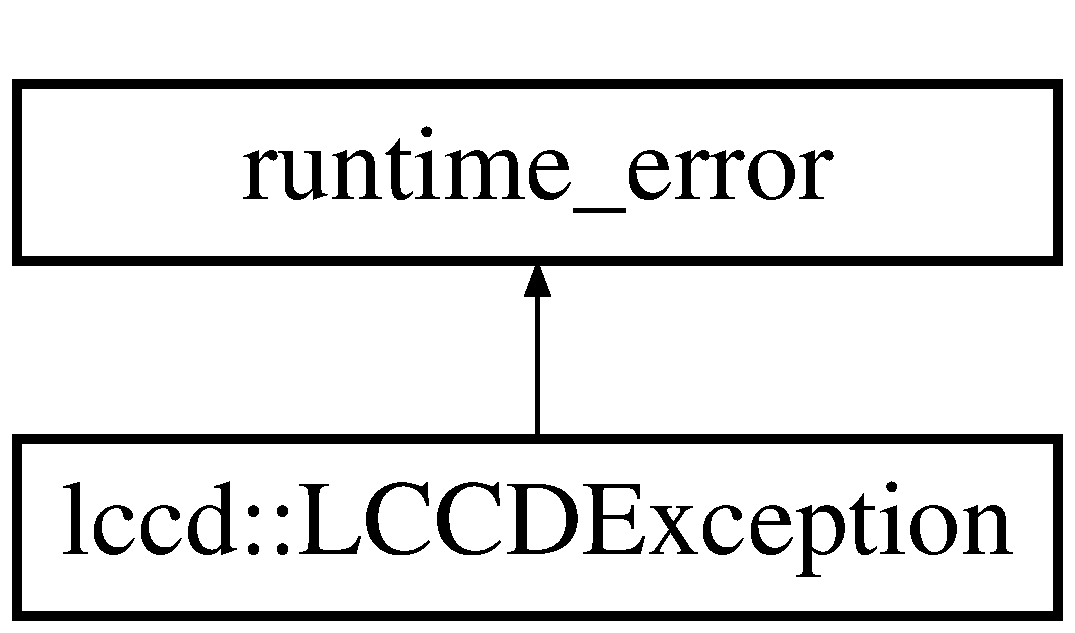
\includegraphics[height=2.000000cm]{classlccd_1_1LCCDException}
\end{center}
\end{figure}
\subsection*{Public Member Functions}
\begin{DoxyCompactItemize}
\item 
{\bfseries L\-C\-C\-D\-Exception} (const std\-::string \&the\-Message, unsigned long the\-Error\-Code)\label{classlccd_1_1LCCDException_afbaaf4e59a2cea7a5a2ec4cc792b2a09}

\item 
virtual const char $\ast$ {\bf get\-Message} () const \label{classlccd_1_1LCCDException_a7c06b227bf3920f9cc92606e25241af8}

\begin{DoxyCompactList}\small\item\em Returns the error message. \end{DoxyCompactList}\item 
virtual unsigned long {\bf get\-Error\-Code} () const \label{classlccd_1_1LCCDException_a856abfa9a886d131e7e39be4ad879a07}

\begin{DoxyCompactList}\small\item\em Returns the error code. \end{DoxyCompactList}\end{DoxyCompactItemize}


\subsection{Detailed Description}
Defines an exception similar to the one defined by the Cond\-D\-B\-My\-S\-Q\-L package. \begin{DoxyAuthor}{Author}
\-: R. P�schl D\-E\-S\-Y (based on a class created by the Cond\-D\-B\-My\-S\-Q\-L team) 
\end{DoxyAuthor}
\begin{DoxyDate}{Date}
Aug 17 2005 
\end{DoxyDate}


Definition at line 18 of file L\-C\-C\-D\-Exception.\-hh.



The documentation for this class was generated from the following file\-:\begin{DoxyCompactItemize}
\item 
/nfs/dust/ilc/user/marquezh/\-Calice\-Soft\-\_\-w\-\_\-\-I\-L\-C\-Soft\-\_\-v02-\/03-\/02/calice\-\_\-db\-\_\-tools/include/L\-C\-C\-D\-Exception.\-hh\end{DoxyCompactItemize}

\section{lccd\-:\-:L\-C\-Cond\-Object Class Reference}
\label{classlccd_1_1LCCondObject}\index{lccd\-::\-L\-C\-Cond\-Object@{lccd\-::\-L\-C\-Cond\-Object}}
Inheritance diagram for lccd\-:\-:L\-C\-Cond\-Object\-:\begin{figure}[H]
\begin{center}
\leavevmode
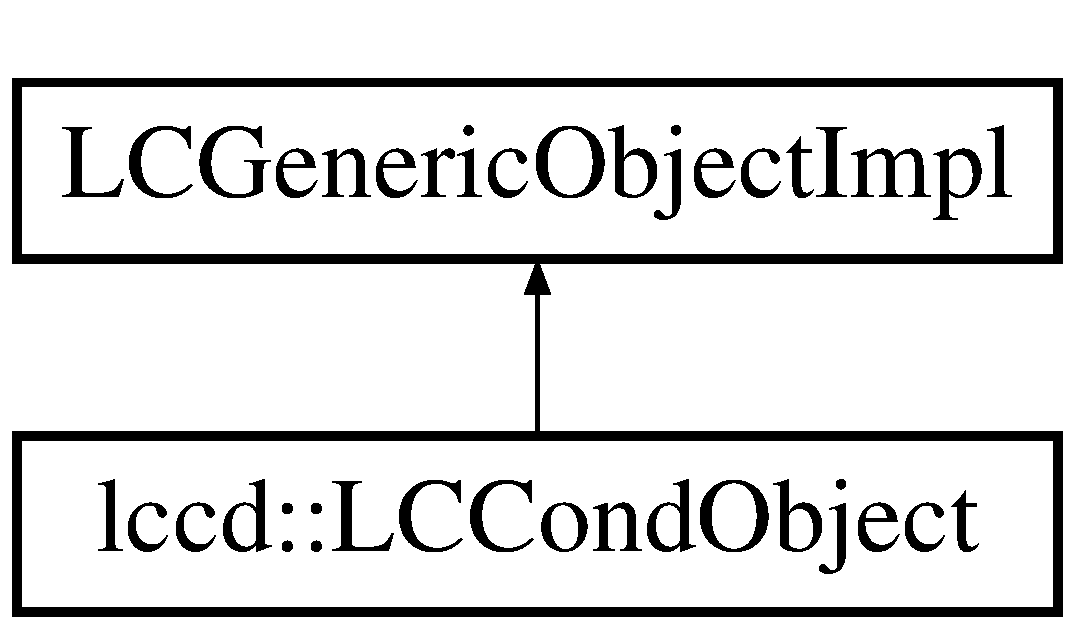
\includegraphics[height=2.000000cm]{classlccd_1_1LCCondObject}
\end{center}
\end{figure}
\subsection*{Public Member Functions}
\begin{DoxyCompactItemize}
\item 
{\bfseries L\-C\-Cond\-Object} (int n\-Int, int n\-Float, int n\-Double)\label{classlccd_1_1LCCondObject_a1068e8d6c4425f9d7de916a4667b3dcd}

\item 
virtual {\bf L\-C\-Cond\-Object} $\ast$ {\bfseries convert} (L\-C\-Object $\ast$obj)\label{classlccd_1_1LCCondObject_a6ea62eaaa3fbeedb6f77e4401600708d}

\item 
virtual void {\bfseries print} (std\-::ostream \&os)\label{classlccd_1_1LCCondObject_a3478d345a4cd72795ce687c204f7dfa1}

\item 
virtual void {\bfseries print\-Hdr} (std\-::ostream \&os)\label{classlccd_1_1LCCondObject_a29da862e8020fb454ba73bc703176598}

\item 
virtual void {\bfseries print\-Tbl} (std\-::ostream \&os)\label{classlccd_1_1LCCondObject_afa59727acd3d00eeac7128ecf7b56b3c}

\item 
virtual void {\bfseries get\-Create\-Query} (std\-::ostream \&os)\label{classlccd_1_1LCCondObject_a8a81b536c8bc22048eb62e1c1e205be5}

\item 
virtual void {\bfseries get\-Insert\-Query} (std\-::ostream \&os)\label{classlccd_1_1LCCondObject_a096e5cd0c805f3272e1c3e374d2d6edc}

\item 
virtual void {\bfseries get\-Drop\-Query} (std\-::ostream \&os)\label{classlccd_1_1LCCondObject_ad7e20f87d4e0cde0e6eac33255ab570c}

\end{DoxyCompactItemize}


\subsection{Detailed Description}


Definition at line 13 of file L\-C\-Cond\-Object.\-hh.



The documentation for this class was generated from the following file\-:\begin{DoxyCompactItemize}
\item 
/nfs/dust/ilc/user/marquezh/\-Calice\-Soft\-\_\-w\-\_\-\-I\-L\-C\-Soft\-\_\-v02-\/03-\/02/calice\-\_\-db\-\_\-tools/include/L\-C\-Cond\-Object.\-hh\end{DoxyCompactItemize}

\section{lccd\-:\-:L\-C\-Cond\-Object\-Mgr Class Reference}
\label{classlccd_1_1LCCondObjectMgr}\index{lccd\-::\-L\-C\-Cond\-Object\-Mgr@{lccd\-::\-L\-C\-Cond\-Object\-Mgr}}
\subsection*{Public Member Functions}
\begin{DoxyCompactItemize}
\item 
void {\bfseries register\-L\-C\-Cond\-Object} ({\bf L\-C\-Cond\-Object} $\ast$obj)\label{classlccd_1_1LCCondObjectMgr_a5b0c841bd7baba67058ff038a37d6bf1}

\item 
void {\bfseries register\-L\-C\-Cond\-Object} ({\bf L\-C\-Cond\-Object} $\ast$obj, const std\-::string \&name)\label{classlccd_1_1LCCondObjectMgr_a8f19da887e6789603d76542f5d6276af}

\item 
void {\bfseries remove\-L\-C\-Cond\-Object} (const std\-::string \&name)\label{classlccd_1_1LCCondObjectMgr_aff3f7984a32c5d22343f20e18899f24d}

\item 
{\bf L\-C\-Cond\-Object} $\ast$ {\bfseries get\-L\-C\-Cond\-Object} (const std\-::string \&name)\label{classlccd_1_1LCCondObjectMgr_adbbd2fc04da7f8051426753accae29ee}

\item 
void {\bfseries clear} ()\label{classlccd_1_1LCCondObjectMgr_af75565bcf3c46cbbed5e667fb5a6e815}

\end{DoxyCompactItemize}
\subsection*{Static Public Member Functions}
\begin{DoxyCompactItemize}
\item 
static {\bf L\-C\-Cond\-Object\-Mgr} $\ast$ {\bfseries instance} ()\label{classlccd_1_1LCCondObjectMgr_a22f8215e23eccae0b5df78077b8f2b38}

\end{DoxyCompactItemize}


\subsection{Detailed Description}


Definition at line 13 of file L\-C\-Cond\-Object\-Mgr.\-hh.



The documentation for this class was generated from the following files\-:\begin{DoxyCompactItemize}
\item 
/nfs/dust/ilc/user/marquezh/\-Calice\-Soft\-\_\-w\-\_\-\-I\-L\-C\-Soft\-\_\-v02-\/03-\/02/calice\-\_\-db\-\_\-tools/include/L\-C\-Cond\-Object\-Mgr.\-hh\item 
/nfs/dust/ilc/user/marquezh/\-Calice\-Soft\-\_\-w\-\_\-\-I\-L\-C\-Soft\-\_\-v02-\/03-\/02/calice\-\_\-db\-\_\-tools/src/L\-C\-Cond\-Object\-Mgr.\-cc\end{DoxyCompactItemize}

\section{Lightyield\-Calculator Class Reference}
\label{classLightyieldCalculator}\index{Lightyield\-Calculator@{Lightyield\-Calculator}}
\subsection*{Public Member Functions}
\begin{DoxyCompactItemize}
\item 
int {\bfseries run} (int argc, char $\ast$$\ast$argv)\label{classLightyieldCalculator_a96fcc722e4ecaa6e5306cd07ca20c914}

\item 
double {\bfseries get\-Value} (const char $\ast$, unsigned int)\label{classLightyieldCalculator_a3882a851b3ea64e88d731cdf53b8d4ff}

\item 
double {\bfseries get\-Value} (const char $\ast$, unsigned int, double)\label{classLightyieldCalculator_af936a6f685c4f12e871ab451ca233c1f}

\item 
double {\bfseries get\-Reference\-Temperature} (const char $\ast$, unsigned int)\label{classLightyieldCalculator_a46ae352a2979a5686aa4e3bcef9bc7f0}

\end{DoxyCompactItemize}
\subsection*{Protected Member Functions}
\begin{DoxyCompactItemize}
\item 
int {\bfseries loop\-All\-Channels} (const char $\ast$=\char`\"{}default\-\_\-ly.\-txt\char`\"{})\label{classLightyieldCalculator_a73a19c47cec74fa49f4af63d2398e5ed}

\end{DoxyCompactItemize}


\subsection{Detailed Description}


Definition at line 30 of file Lightyield\-Calculator.\-hh.



The documentation for this class was generated from the following files\-:\begin{DoxyCompactItemize}
\item 
/nfs/dust/ilc/user/marquezh/\-Calice\-Soft\-\_\-w\-\_\-\-I\-L\-C\-Soft\-\_\-v02-\/03-\/02/calice\-\_\-db\-\_\-tools/include/{\bf Lightyield\-Calculator.\-hh}\item 
/nfs/dust/ilc/user/marquezh/\-Calice\-Soft\-\_\-w\-\_\-\-I\-L\-C\-Soft\-\_\-v02-\/03-\/02/calice\-\_\-db\-\_\-tools/src/Lightyield\-Calculator.\-cc\end{DoxyCompactItemize}

\section{C\-A\-L\-I\-C\-E\-:\-:Non\-Supported\-Run\-Number\-Exception Class Reference}
\label{classCALICE_1_1NonSupportedRunNumberException}\index{C\-A\-L\-I\-C\-E\-::\-Non\-Supported\-Run\-Number\-Exception@{C\-A\-L\-I\-C\-E\-::\-Non\-Supported\-Run\-Number\-Exception}}


exception to be thrown if the given run\-Number is not supported  




{\ttfamily \#include $<$D\-B\-Exception.\-hh$>$}

Inheritance diagram for C\-A\-L\-I\-C\-E\-:\-:Non\-Supported\-Run\-Number\-Exception\-:\begin{figure}[H]
\begin{center}
\leavevmode
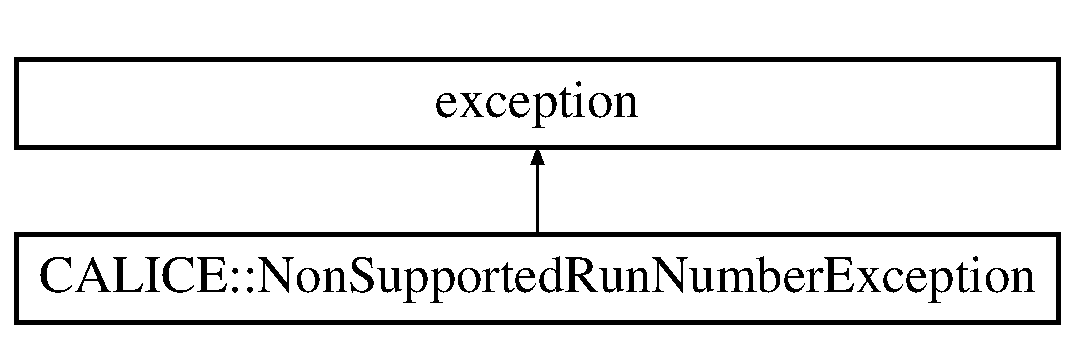
\includegraphics[height=2.000000cm]{classCALICE_1_1NonSupportedRunNumberException}
\end{center}
\end{figure}
\subsection*{Public Member Functions}
\begin{DoxyCompactItemize}
\item 
{\bfseries Non\-Supported\-Run\-Number\-Exception} (std\-::string text)  throw ()\label{classCALICE_1_1NonSupportedRunNumberException_a8930360bfbe77fc806d31f4552b99433}

\item 
const char $\ast$ {\bfseries what} () const   throw ()\label{classCALICE_1_1NonSupportedRunNumberException_a696cc733eb1fd74d2a33ffa5140e9563}

\end{DoxyCompactItemize}
\subsection*{Protected Attributes}
\begin{DoxyCompactItemize}
\item 
std\-::string {\bfseries \-\_\-message}\label{classCALICE_1_1NonSupportedRunNumberException_ad2f56451dab096208bae9e3e3b653dce}

\end{DoxyCompactItemize}


\subsection{Detailed Description}
exception to be thrown if the given run\-Number is not supported 

Definition at line 14 of file D\-B\-Exception.\-hh.



The documentation for this class was generated from the following file\-:\begin{DoxyCompactItemize}
\item 
/nfs/dust/ilc/user/marquezh/\-Calice\-Soft\-\_\-w\-\_\-\-I\-L\-C\-Soft\-\_\-v02-\/03-\/02/calice\-\_\-db\-\_\-tools/include/D\-B\-Exception.\-hh\end{DoxyCompactItemize}

\section{Relative\-Slopes\-Calculator Class Reference}
\label{classRelativeSlopesCalculator}\index{Relative\-Slopes\-Calculator@{Relative\-Slopes\-Calculator}}
\subsection*{Public Member Functions}
\begin{DoxyCompactItemize}
\item 
int {\bfseries run} (int argc, char $\ast$$\ast$argv)\label{classRelativeSlopesCalculator_afe80265289b375bdf3473268421ef6f8}

\item 
double {\bfseries get\-Value} (const char $\ast$, unsigned int)\label{classRelativeSlopesCalculator_a37ec713046ab2a219da5202614a74c04}

\item 
double {\bfseries get\-Value} (const char $\ast$, unsigned int, double)\label{classRelativeSlopesCalculator_ae55520b72d509a5aa668aa666942a582}

\item 
double {\bfseries get\-Reference\-Temperature} (const char $\ast$, unsigned int)\label{classRelativeSlopesCalculator_a952b021211863b57ff58db16c599e51a}

\end{DoxyCompactItemize}
\subsection*{Protected Member Functions}
\begin{DoxyCompactItemize}
\item 
int {\bfseries loop\-All\-Channels} (const char $\ast$=\char`\"{}default\-\_\-rel\-\_\-slopes.\-txt\char`\"{})\label{classRelativeSlopesCalculator_ab332e02dc1327d6b825c8a316a1aca5d}

\end{DoxyCompactItemize}


\subsection{Detailed Description}


Definition at line 28 of file Relative\-Slopes\-Calculator.\-hh.



The documentation for this class was generated from the following files\-:\begin{DoxyCompactItemize}
\item 
/nfs/dust/ilc/user/marquezh/\-Calice\-Soft\-\_\-w\-\_\-\-I\-L\-C\-Soft\-\_\-v02-\/03-\/02/calice\-\_\-db\-\_\-tools/include/{\bf Relative\-Slopes\-Calculator.\-hh}\item 
/nfs/dust/ilc/user/marquezh/\-Calice\-Soft\-\_\-w\-\_\-\-I\-L\-C\-Soft\-\_\-v02-\/03-\/02/calice\-\_\-db\-\_\-tools/src/Relative\-Slopes\-Calculator.\-cc\end{DoxyCompactItemize}

\section{Shift\-Linear\-Fit\-Constants Class Reference}
\label{classShiftLinearFitConstants}\index{Shift\-Linear\-Fit\-Constants@{Shift\-Linear\-Fit\-Constants}}
\subsection*{Public Member Functions}
\begin{DoxyCompactItemize}
\item 
int {\bfseries run} (int argc, char $\ast$$\ast$argv)\label{classShiftLinearFitConstants_a87df3cbfbd584a8506662b2c5ae5ab2b}

\item 
double {\bfseries get\-Value} (unsigned int, double)\label{classShiftLinearFitConstants_ad6c9887ba7691ffd393d3a30bd28c4b8}

\item 
double {\bfseries get\-Ref\-Temp} (unsigned int)\label{classShiftLinearFitConstants_a357bca386c28b29a5d897dd5389b9c94}

\end{DoxyCompactItemize}
\subsection*{Protected Member Functions}
\begin{DoxyCompactItemize}
\item 
int {\bfseries loop\-All\-Channels} (const char $\ast$=\char`\"{}default\-\_\-lfc\-\_\-shifted.\-txt\char`\"{})\label{classShiftLinearFitConstants_a4c83bab781c2054dde88cb69dc03f01c}

\end{DoxyCompactItemize}


\subsection{Detailed Description}


Definition at line 31 of file Shift\-Linear\-Fit\-Constants.\-hh.



The documentation for this class was generated from the following files\-:\begin{DoxyCompactItemize}
\item 
/nfs/dust/ilc/user/marquezh/\-Calice\-Soft\-\_\-w\-\_\-\-I\-L\-C\-Soft\-\_\-v02-\/03-\/02/calice\-\_\-db\-\_\-tools/include/{\bf Shift\-Linear\-Fit\-Constants.\-hh}\item 
/nfs/dust/ilc/user/marquezh/\-Calice\-Soft\-\_\-w\-\_\-\-I\-L\-C\-Soft\-\_\-v02-\/03-\/02/calice\-\_\-db\-\_\-tools/src/Shift\-Linear\-Fit\-Constants.\-cc\end{DoxyCompactItemize}

\section{Simple\-File\-Writer Class Reference}
\label{classSimpleFileWriter}\index{Simple\-File\-Writer@{Simple\-File\-Writer}}


{\ttfamily \#include $<$Simple\-File\-Writer.\-hh$>$}

\subsection*{Public Member Functions}
\begin{DoxyCompactItemize}
\item 
{\bf Simple\-File\-Writer} ()
\item 
{\bfseries Simple\-File\-Writer} (const std\-::string \&file)\label{classSimpleFileWriter_aaa81aa77699063edff9e1b0b2c83be3c}

\item 
{\bf Simple\-File\-Writer} \& {\bfseries set\-File} (const std\-::string \&file)\label{classSimpleFileWriter_a86410980c38a2199324a4b281439c63d}

\item 
{\bf Simple\-File\-Writer} \& {\bfseries write\-Collection} (E\-V\-E\-N\-T\-::\-L\-C\-Collection $\ast$col, const std\-::string name)\label{classSimpleFileWriter_a7b384ee227ea72cd56b1994b8aa96f8b}

\item 
{\bf Simple\-File\-Writer} \& {\bfseries print} (std\-::ostream \&os)\label{classSimpleFileWriter_af76ab8c59d7fb319bc58a8593db9c8cb}

\end{DoxyCompactItemize}


\subsection{Detailed Description}
\begin{DoxyRefDesc}{Todo}
\item[{\bf Todo}]\-: move this tool to calice\-\_\-cddata \end{DoxyRefDesc}
Documentation missing. \begin{DoxyRefDesc}{Todo}
\item[{\bf Todo}]Write documentation!\end{DoxyRefDesc}


Definition at line 16 of file Simple\-File\-Writer.\-hh.



\subsection{Constructor \& Destructor Documentation}
\index{Simple\-File\-Writer@{Simple\-File\-Writer}!Simple\-File\-Writer@{Simple\-File\-Writer}}
\index{Simple\-File\-Writer@{Simple\-File\-Writer}!SimpleFileWriter@{Simple\-File\-Writer}}
\subsubsection[{Simple\-File\-Writer}]{\setlength{\rightskip}{0pt plus 5cm}Simple\-File\-Writer\-::\-Simple\-File\-Writer (
\begin{DoxyParamCaption}
{}
\end{DoxyParamCaption}
)}\label{classSimpleFileWriter_a80ae7a5b171b5cf0bb71167da397b827}
\begin{DoxyRefDesc}{Todo}
\item[{\bf Todo}]\-: move this tool to calice\-\_\-cddata \end{DoxyRefDesc}


Definition at line 10 of file Simple\-File\-Writer.\-cc.



The documentation for this class was generated from the following files\-:\begin{DoxyCompactItemize}
\item 
/nfs/dust/ilc/user/marquezh/\-Calice\-Soft\-\_\-w\-\_\-\-I\-L\-C\-Soft\-\_\-v02-\/03-\/02/calice\-\_\-db\-\_\-tools/include/Simple\-File\-Writer.\-hh\item 
/nfs/dust/ilc/user/marquezh/\-Calice\-Soft\-\_\-w\-\_\-\-I\-L\-C\-Soft\-\_\-v02-\/03-\/02/calice\-\_\-db\-\_\-tools/src/Simple\-File\-Writer.\-cc\end{DoxyCompactItemize}

\section{slope\-Struct Struct Reference}
\label{structslopeStruct}\index{slope\-Struct@{slope\-Struct}}
\subsection*{Public Attributes}
\begin{DoxyCompactItemize}
\item 
int {\bfseries id}\label{structslopeStruct_ad71a3bb481c5f47380ddbbdf5b5042e3}

\item 
float {\bfseries calib}\label{structslopeStruct_a5a7227374a824eccdeb55bb4006bddff}

\item 
float {\bfseries calib\-Error}\label{structslopeStruct_a0a0c951def9045453f543f077f1879a8}

\item 
float {\bfseries relative\-Slope}\label{structslopeStruct_ab27f75ceb2fd2dc358d0733b2cfb5f8d}

\item 
float {\bfseries relative\-Slope\-Error}\label{structslopeStruct_a4fd2eacc2a7e13ecb52ced63ec46766e}

\end{DoxyCompactItemize}


\subsection{Detailed Description}


Definition at line 20 of file Hcal\-Slopes\-Per\-Layer\-Calculator.\-cc.



The documentation for this struct was generated from the following file\-:\begin{DoxyCompactItemize}
\item 
/nfs/dust/ilc/user/marquezh/\-Calice\-Soft\-\_\-w\-\_\-\-I\-L\-C\-Soft\-\_\-v02-\/03-\/02/calice\-\_\-db\-\_\-tools/src/Hcal\-Slopes\-Per\-Layer\-Calculator.\-cc\end{DoxyCompactItemize}

\section{s\-Voltages Struct Reference}
\label{structsVoltages}\index{s\-Voltages@{s\-Voltages}}
\subsection*{Public Member Functions}
\begin{DoxyCompactItemize}
\item 
{\bfseries s\-Voltages} (unsigned int mod, double v\-\_\-\-A, double v\-\_\-\-B)\label{structsVoltages_abd71bedce816007146b3185cf1941e77}

\end{DoxyCompactItemize}
\subsection*{Public Attributes}
\begin{DoxyCompactItemize}
\item 
unsigned int {\bfseries module}\label{structsVoltages_a467add2524f32aa080c2e2e91f6c0669}

\item 
double {\bfseries voltage\-\_\-\-A}\label{structsVoltages_acee26f5fd14bf3e58b65d736bd40d9aa}

\item 
double {\bfseries voltage\-\_\-\-B}\label{structsVoltages_ae2e8a6ec429c790474887aaaefd821bb}

\end{DoxyCompactItemize}


\subsection{Detailed Description}


Definition at line 66 of file display\-Run\-Info.\-cc.



The documentation for this struct was generated from the following file\-:\begin{DoxyCompactItemize}
\item 
/nfs/dust/ilc/user/marquezh/\-Calice\-Soft\-\_\-w\-\_\-\-I\-L\-C\-Soft\-\_\-v02-\/03-\/02/calice\-\_\-db\-\_\-tools/src/{\bf display\-Run\-Info.\-cc}\end{DoxyCompactItemize}

\section{Syntax Class Reference}
\label{classSyntax}\index{Syntax@{Syntax}}
\subsection*{Public Member Functions}
\begin{DoxyCompactItemize}
\item 
{\bfseries Syntax} (string str)\label{classSyntax_aa98349efaef7b45bbdcd10f495d734e2}

\item 
string \& {\bfseries get\-Message} ()\label{classSyntax_a971f81d4ddd5333cf22ab48334d9f74a}

\end{DoxyCompactItemize}


\subsection{Detailed Description}


Definition at line 173 of file cdbadmin.\-cc.



The documentation for this class was generated from the following file\-:\begin{DoxyCompactItemize}
\item 
/nfs/dust/ilc/user/marquezh/\-Calice\-Soft\-\_\-w\-\_\-\-I\-L\-C\-Soft\-\_\-v02-\/03-\/02/calice\-\_\-db\-\_\-tools/src/cdbadmin.\-cc\end{DoxyCompactItemize}

\section{Time\-String Class Reference}
\label{classTimeString}\index{Time\-String@{Time\-String}}


{\ttfamily \#include $<$Time\-String.\-hh$>$}

\subsection*{Public Member Functions}
\begin{DoxyCompactItemize}
\item 
{\bfseries Time\-String} (const std\-::string str)\label{classTimeString_a60433b1fbd3e0e4d2de19332832c4d36}

\item 
const lcio\-::long64 {\bfseries get\-Time\-Stamp} () const \label{classTimeString_ae847cb33e3f42037565f0aebec804d6f}

\item 
const lcio\-::\-L\-C\-Time {\bfseries get\-L\-C\-Time} () const \label{classTimeString_a9ceb7a98daa11f704edaec9f5793178f}

\end{DoxyCompactItemize}


\subsection{Detailed Description}
Documentation missing. \begin{DoxyRefDesc}{Todo}
\item[{\bf Todo}]Write documentation!\end{DoxyRefDesc}


Definition at line 13 of file Time\-String.\-hh.



The documentation for this class was generated from the following files\-:\begin{DoxyCompactItemize}
\item 
/nfs/dust/ilc/user/marquezh/\-Calice\-Soft\-\_\-w\-\_\-\-I\-L\-C\-Soft\-\_\-v02-\/03-\/02/calice\-\_\-db\-\_\-tools/include/Time\-String.\-hh\item 
/nfs/dust/ilc/user/marquezh/\-Calice\-Soft\-\_\-w\-\_\-\-I\-L\-C\-Soft\-\_\-v02-\/03-\/02/calice\-\_\-db\-\_\-tools/src/Time\-String.\-cc\end{DoxyCompactItemize}

\section{Transport\-Linear\-Fit\-Constants Class Reference}
\label{classTransportLinearFitConstants}\index{Transport\-Linear\-Fit\-Constants@{Transport\-Linear\-Fit\-Constants}}
\subsection*{Public Member Functions}
\begin{DoxyCompactItemize}
\item 
int {\bfseries run} (int argc, char $\ast$$\ast$argv)\label{classTransportLinearFitConstants_a67394310263e6a5c9df72c7567127268}

\item 
void {\bfseries get\-Value} (const unsigned int, float \&, float \&, float \&, float \&)\label{classTransportLinearFitConstants_a0f28ea80602c327124ed9644467e7d2b}

\end{DoxyCompactItemize}
\subsection*{Protected Member Functions}
\begin{DoxyCompactItemize}
\item 
int {\bfseries loop\-All\-Channels} (const char $\ast$=\char`\"{}default\-\_\-lfc\-\_\-transported.\-txt\char`\"{})\label{classTransportLinearFitConstants_a9ff5f5a3a1533bf51f187f382becbc4d}

\end{DoxyCompactItemize}


\subsection{Detailed Description}


Definition at line 30 of file Transport\-Linear\-Fit\-Constants.\-hh.



The documentation for this class was generated from the following files\-:\begin{DoxyCompactItemize}
\item 
/nfs/dust/ilc/user/marquezh/\-Calice\-Soft\-\_\-w\-\_\-\-I\-L\-C\-Soft\-\_\-v02-\/03-\/02/calice\-\_\-db\-\_\-tools/include/{\bf Transport\-Linear\-Fit\-Constants.\-hh}\item 
/nfs/dust/ilc/user/marquezh/\-Calice\-Soft\-\_\-w\-\_\-\-I\-L\-C\-Soft\-\_\-v02-\/03-\/02/calice\-\_\-db\-\_\-tools/src/Transport\-Linear\-Fit\-Constants.\-cc\end{DoxyCompactItemize}

\section{Trigger\-Input Class Reference}
\label{classTriggerInput}\index{Trigger\-Input@{Trigger\-Input}}


{\ttfamily \#include $<$Trigger\-Input.\-hh$>$}

\subsection*{Public Member Functions}
\begin{DoxyCompactItemize}
\item 
{\bfseries Trigger\-Input} (const std\-::string \&device, const int pin, const int delay=0, const int jitter=1)\label{classTriggerInput_a6134822cc4ebfbdbeabfb445486add7a}

\item 
std\-::ostream \& {\bfseries print} (std\-::ostream \&out) const \label{classTriggerInput_ac491cff98d85e24c22be0dd3ed8f0f62}

\end{DoxyCompactItemize}


\subsection{Detailed Description}
Documentation missing. \begin{DoxyRefDesc}{Todo}
\item[{\bf Todo}]Write documentation!\end{DoxyRefDesc}


Definition at line 12 of file Trigger\-Input.\-hh.



The documentation for this class was generated from the following files\-:\begin{DoxyCompactItemize}
\item 
/nfs/dust/ilc/user/marquezh/\-Calice\-Soft\-\_\-w\-\_\-\-I\-L\-C\-Soft\-\_\-v02-\/03-\/02/calice\-\_\-db\-\_\-tools/include/Trigger\-Input.\-hh\item 
/nfs/dust/ilc/user/marquezh/\-Calice\-Soft\-\_\-w\-\_\-\-I\-L\-C\-Soft\-\_\-v02-\/03-\/02/calice\-\_\-db\-\_\-tools/src/Trigger\-Input.\-cc\end{DoxyCompactItemize}

\section{Trigger\-Map Class Reference}
\label{classTriggerMap}\index{Trigger\-Map@{Trigger\-Map}}


{\ttfamily \#include $<$Trigger\-Map.\-hh$>$}

\subsection*{Public Member Functions}
\begin{DoxyCompactItemize}
\item 
{\bfseries Trigger\-Map} (E\-V\-E\-N\-T\-::\-L\-C\-Collection $\ast$col)\label{classTriggerMap_a23752fc2e02a6689cfdb5014cc5e1a5d}

\item 
std\-::ostream \& {\bfseries print} (std\-::ostream \&out) const \label{classTriggerMap_aef710938c4e2d4c367aabb57a41ca66b}

\end{DoxyCompactItemize}


\subsection{Detailed Description}
Documentation missing. \begin{DoxyRefDesc}{Todo}
\item[{\bf Todo}]Write documentation!\end{DoxyRefDesc}


Definition at line 14 of file Trigger\-Map.\-hh.



The documentation for this class was generated from the following files\-:\begin{DoxyCompactItemize}
\item 
/nfs/dust/ilc/user/marquezh/\-Calice\-Soft\-\_\-w\-\_\-\-I\-L\-C\-Soft\-\_\-v02-\/03-\/02/calice\-\_\-db\-\_\-tools/include/Trigger\-Map.\-hh\item 
/nfs/dust/ilc/user/marquezh/\-Calice\-Soft\-\_\-w\-\_\-\-I\-L\-C\-Soft\-\_\-v02-\/03-\/02/calice\-\_\-db\-\_\-tools/src/Trigger\-Map.\-cc\end{DoxyCompactItemize}

\section{voltage\-Data\-\_\-t Struct Reference}
\label{structvoltageData__t}\index{voltage\-Data\-\_\-t@{voltage\-Data\-\_\-t}}
\subsection*{Public Attributes}
\begin{DoxyCompactItemize}
\item 
std\-::vector$<$ double $>$ {\bfseries A}\label{structvoltageData__t_a56e10365b70d9e59f142cb9084621bed}

\item 
std\-::vector$<$ double $>$ {\bfseries B}\label{structvoltageData__t_a44e974fb0b6035c3000d0a59abaca721}

\end{DoxyCompactItemize}


\subsection{Detailed Description}


Definition at line 92 of file extract\-Gain\-Vs\-Temp.\-cc.



The documentation for this struct was generated from the following file\-:\begin{DoxyCompactItemize}
\item 
/nfs/dust/ilc/user/marquezh/\-Calice\-Soft\-\_\-w\-\_\-\-I\-L\-C\-Soft\-\_\-v02-\/03-\/02/calice\-\_\-db\-\_\-tools/src/{\bf extract\-Gain\-Vs\-Temp.\-cc}\end{DoxyCompactItemize}

\chapter{File Documentation}
\section{/nfs/dust/ilc/user/marquezh/\-Calice\-Soft\-\_\-w\-\_\-\-I\-L\-C\-Soft\-\_\-v02-\/03-\/02/calice\-\_\-db\-\_\-tools/include/\-Absolute\-Slopes\-Calculator.hh File Reference}
\label{AbsoluteSlopesCalculator_8hh}\index{/nfs/dust/ilc/user/marquezh/\-Calice\-Soft\-\_\-w\-\_\-\-I\-L\-C\-Soft\-\_\-v02-\/03-\/02/calice\-\_\-db\-\_\-tools/include/\-Absolute\-Slopes\-Calculator.\-hh@{/nfs/dust/ilc/user/marquezh/\-Calice\-Soft\-\_\-w\-\_\-\-I\-L\-C\-Soft\-\_\-v02-\/03-\/02/calice\-\_\-db\-\_\-tools/include/\-Absolute\-Slopes\-Calculator.\-hh}}
{\ttfamily \#include \char`\"{}Linear\-Fit\-Constant.\-hh\char`\"{}}\\*
{\ttfamily \#include \char`\"{}Access\-Linear\-Fit\-Constant.\-hh\char`\"{}}\\*
{\ttfamily \#include \char`\"{}lcio.\-h\char`\"{}}\\*
{\ttfamily \#include \char`\"{}I\-M\-P\-L/\-L\-C\-Collection\-Vec.\-h\char`\"{}}\\*
{\ttfamily \#include \char`\"{}I\-M\-P\-L/\-L\-C\-T\-O\-O\-L\-S.\-h\char`\"{}}\\*
{\ttfamily \#include \char`\"{}I\-O/\-L\-C\-Reader.\-h\char`\"{}}\\*
\subsection*{Classes}
\begin{DoxyCompactItemize}
\item 
class {\bf Absolute\-Slopes\-Calculator}
\end{DoxyCompactItemize}


\subsection{Detailed Description}
This tool calculates absolute slopes from C\-A\-L\-I\-C\-E\-::\-Linear\-Fit\-Constants

Command line parameters\-: \par
 {\itshape --rel\-\_\-slope} $<$float$>$ -\/$>$ define relative slope for all channels\par
\par
 {\itshape --const} -\/$>$ define input for constant \par
\par
 {\itshape --txt} $<$inputfile.\-txt$>$ -\/$>$ define .txt file as source (format\-: module/chip/channel/value/error...) \par
 {\itshape --slcio} $<$inputfile.\-slcio$>$ $<$collection$>$ -\/$>$ define collection from .slcio file as source \par
 {\itshape --db} $<$D\-Bfolder$>$ $<$time$>$ -\/$>$ define database folder at time $<$time$>$ as source, using no tag \par
 {\itshape --db\-\_\-tag} $<$D\-Bfolder$>$ $<$time$>$ $<$tag$>$ -\/$>$ define database folder at time $<$time$>$ and tag $<$tag$>$ as source \par


Definition in file {\bf Absolute\-Slopes\-Calculator.\-hh}.


\section{/nfs/dust/ilc/user/marquezh/\-Calice\-Soft\-\_\-w\-\_\-\-I\-L\-C\-Soft\-\_\-v02-\/03-\/02/calice\-\_\-db\-\_\-tools/include/\-Average\-Linear\-Fit\-Slopes.hh File Reference}
\label{AverageLinearFitSlopes_8hh}\index{/nfs/dust/ilc/user/marquezh/\-Calice\-Soft\-\_\-w\-\_\-\-I\-L\-C\-Soft\-\_\-v02-\/03-\/02/calice\-\_\-db\-\_\-tools/include/\-Average\-Linear\-Fit\-Slopes.\-hh@{/nfs/dust/ilc/user/marquezh/\-Calice\-Soft\-\_\-w\-\_\-\-I\-L\-C\-Soft\-\_\-v02-\/03-\/02/calice\-\_\-db\-\_\-tools/include/\-Average\-Linear\-Fit\-Slopes.\-hh}}
{\ttfamily \#include \char`\"{}Linear\-Fit\-Slope.\-hh\char`\"{}}\\*
{\ttfamily \#include \char`\"{}Access\-Linear\-Fit\-Slope.\-hh\char`\"{}}\\*
{\ttfamily \#include \char`\"{}lcio.\-h\char`\"{}}\\*
{\ttfamily \#include \char`\"{}I\-M\-P\-L/\-L\-C\-Collection\-Vec.\-h\char`\"{}}\\*
{\ttfamily \#include \char`\"{}I\-M\-P\-L/\-L\-C\-T\-O\-O\-L\-S.\-h\char`\"{}}\\*
{\ttfamily \#include \char`\"{}I\-O/\-L\-C\-Reader.\-h\char`\"{}}\\*
\subsection*{Classes}
\begin{DoxyCompactItemize}
\item 
class {\bf Average\-Linear\-Fit\-Slopes}
\end{DoxyCompactItemize}


\subsection{Detailed Description}
This tool calculates the average of n sets of C\-A\-L\-I\-C\-E\-::\-Linear\-Fit\-Slopes.

Command line parameters\-:\par
\par
 /e --val -\/$>$ add new value for average\par
\par
 /e --txt $<$inputfile.\-txt$>$ -\/$>$ define .txt file as source (format\-: module/chip/channel/value/error...)\par
 /e --slcio $<$inputfile.\-slcio$>$ $<$collection$>$ -\/$>$ define collection from .slcio file as source\par
 /e --db $<$D\-Bfolder$>$ $<$time$>$ -\/$>$ define database folder at time $<$time$>$ as source, using no tag\par
 /e --db\-\_\-tag $<$D\-Bfolder$>$ $<$time$>$ $<$tag$>$ -\/$>$ define database folder at time $<$time$>$ and tag $<$tag$>$ as source\par


Definition in file {\bf Average\-Linear\-Fit\-Slopes.\-hh}.


\section{/nfs/dust/ilc/user/marquezh/\-Calice\-Soft\-\_\-w\-\_\-\-I\-L\-C\-Soft\-\_\-v02-\/03-\/02/calice\-\_\-db\-\_\-tools/include/\-Compare\-Linear\-Fit\-Constants.hh File Reference}
\label{include_2CompareLinearFitConstants_8hh}\index{/nfs/dust/ilc/user/marquezh/\-Calice\-Soft\-\_\-w\-\_\-\-I\-L\-C\-Soft\-\_\-v02-\/03-\/02/calice\-\_\-db\-\_\-tools/include/\-Compare\-Linear\-Fit\-Constants.\-hh@{/nfs/dust/ilc/user/marquezh/\-Calice\-Soft\-\_\-w\-\_\-\-I\-L\-C\-Soft\-\_\-v02-\/03-\/02/calice\-\_\-db\-\_\-tools/include/\-Compare\-Linear\-Fit\-Constants.\-hh}}
{\ttfamily \#include \char`\"{}Linear\-Fit\-Constant.\-hh\char`\"{}}\\*
{\ttfamily \#include \char`\"{}Access\-Linear\-Fit\-Constant.\-hh\char`\"{}}\\*
{\ttfamily \#include \char`\"{}lcio.\-h\char`\"{}}\\*
{\ttfamily \#include \char`\"{}I\-M\-P\-L/\-L\-C\-Collection\-Vec.\-h\char`\"{}}\\*
{\ttfamily \#include \char`\"{}I\-M\-P\-L/\-L\-C\-T\-O\-O\-L\-S.\-h\char`\"{}}\\*
{\ttfamily \#include \char`\"{}I\-O/\-L\-C\-Reader.\-h\char`\"{}}\\*
\subsection*{Classes}
\begin{DoxyCompactItemize}
\item 
class {\bf Compare\-Linear\-Fit\-Constants}
\end{DoxyCompactItemize}


\subsection{Detailed Description}
This tool compares two sets of C\-A\-L\-I\-C\-E\-::\-Linear\-Fit\-Constants.

Command line parameters\-: \begin{DoxyVerb}\e --label1  -\> define label for VAL1) \n
\e --label2  -\> define label for VAL2 \n

\e --val1     -\> define VAL1 input \n
\e --val2     -\> define VAL2 input \n

\e --txt \<inputfile.txt\>                      -> define .txt file as source (format: module/chip/channel/value/error...) \n
\e --slcio \<inputfile.slcio\> \<collection\>   -> define collection from .slcio file as source \n
\e --db \<DBfolder\> \<time\>                   -> define database folder at time \<time\> as source, using no tag \n
\e --db_tag \<DBfolder\> \<time\> \<tag\>       -> define database folder at time \<time\> and tag \<tag\> as source \n\end{DoxyVerb}


Definition in file {\bf Compare\-Linear\-Fit\-Constants.\-hh}.


\section{/nfs/dust/ilc/user/marquezh/\-Calice\-Soft\-\_\-w\-\_\-\-I\-L\-C\-Soft\-\_\-v02-\/03-\/02/calice\-\_\-db\-\_\-tools/include/\-Compare\-Linear\-Fit\-Slopes.hh File Reference}
\label{CompareLinearFitSlopes_8hh}\index{/nfs/dust/ilc/user/marquezh/\-Calice\-Soft\-\_\-w\-\_\-\-I\-L\-C\-Soft\-\_\-v02-\/03-\/02/calice\-\_\-db\-\_\-tools/include/\-Compare\-Linear\-Fit\-Slopes.\-hh@{/nfs/dust/ilc/user/marquezh/\-Calice\-Soft\-\_\-w\-\_\-\-I\-L\-C\-Soft\-\_\-v02-\/03-\/02/calice\-\_\-db\-\_\-tools/include/\-Compare\-Linear\-Fit\-Slopes.\-hh}}
{\ttfamily \#include \char`\"{}Linear\-Fit\-Slope.\-hh\char`\"{}}\\*
{\ttfamily \#include \char`\"{}Access\-Linear\-Fit\-Slope.\-hh\char`\"{}}\\*
{\ttfamily \#include \char`\"{}lcio.\-h\char`\"{}}\\*
{\ttfamily \#include \char`\"{}I\-M\-P\-L/\-L\-C\-Collection\-Vec.\-h\char`\"{}}\\*
{\ttfamily \#include \char`\"{}I\-M\-P\-L/\-L\-C\-T\-O\-O\-L\-S.\-h\char`\"{}}\\*
{\ttfamily \#include \char`\"{}I\-O/\-L\-C\-Reader.\-h\char`\"{}}\\*
\subsection*{Classes}
\begin{DoxyCompactItemize}
\item 
class {\bf Compare\-Linear\-Fit\-Slopes}
\end{DoxyCompactItemize}


\subsection{Detailed Description}
This tool compares two sets of C\-A\-L\-I\-C\-E\-::\-Linear\-Fit\-Slopes.

Command line parameters\-:\par
\par
 {\itshape --label1} -\/$>$ define label for V\-A\-L1\par
 {\itshape --label2} -\/$>$ define label for V\-A\-L2\par
 {\itshape --val1} -\/$>$ define V\-A\-L1 input\par
 {\itshape --val2} -\/$>$ define V\-A\-L2 input\par
\par
 {\itshape --txt} $<$inputfile.\-txt$>$ -\/$>$ define .txt file as source (format\-: module/chip/channel/value/error...)\par
 {\itshape --slcio} $<$inputfile.\-slcio$>$ $<$collection$>$ -\/$>$ define collection from .slcio file as source\par
 {\itshape --db} $<$D\-Bfolder$>$ $<$time$>$ -\/$>$ define database folder at time $<$time$>$ as source, using no tag\par
 {\itshape --db\-\_\-tag} $<$D\-Bfolder$>$ $<$time$>$ $<$tag$>$ -\/$>$ define database folder at time $<$time$>$ and tag $<$tag$>$ as source\par


Definition in file {\bf Compare\-Linear\-Fit\-Slopes.\-hh}.


\section{/nfs/dust/ilc/user/marquezh/\-Calice\-Soft\-\_\-w\-\_\-\-I\-L\-C\-Soft\-\_\-v02-\/03-\/02/calice\-\_\-db\-\_\-tools/include/\-Lightyield\-Calculator.hh File Reference}
\label{LightyieldCalculator_8hh}\index{/nfs/dust/ilc/user/marquezh/\-Calice\-Soft\-\_\-w\-\_\-\-I\-L\-C\-Soft\-\_\-v02-\/03-\/02/calice\-\_\-db\-\_\-tools/include/\-Lightyield\-Calculator.\-hh@{/nfs/dust/ilc/user/marquezh/\-Calice\-Soft\-\_\-w\-\_\-\-I\-L\-C\-Soft\-\_\-v02-\/03-\/02/calice\-\_\-db\-\_\-tools/include/\-Lightyield\-Calculator.\-hh}}
{\ttfamily \#include \char`\"{}Linear\-Fit\-Constant.\-hh\char`\"{}}\\*
{\ttfamily \#include \char`\"{}Access\-Linear\-Fit\-Constant.\-hh\char`\"{}}\\*
{\ttfamily \#include \char`\"{}Access\-Linear\-Fit\-Slope.\-hh\char`\"{}}\\*
{\ttfamily \#include \char`\"{}lcio.\-h\char`\"{}}\\*
{\ttfamily \#include \char`\"{}I\-M\-P\-L/\-L\-C\-Collection\-Vec.\-h\char`\"{}}\\*
{\ttfamily \#include \char`\"{}I\-M\-P\-L/\-L\-C\-T\-O\-O\-L\-S.\-h\char`\"{}}\\*
{\ttfamily \#include \char`\"{}I\-O/\-L\-C\-Reader.\-h\char`\"{}}\\*
\subsection*{Classes}
\begin{DoxyCompactItemize}
\item 
class {\bf Lightyield\-Calculator}
\end{DoxyCompactItemize}


\subsection{Detailed Description}
this tool calculates the lightyield from C\-A\-L\-I\-C\-E\-::\-Linear\-Fit\-Constants.

command line parameters\-:

{\itshape --temp\-\_\-corr} -\/$>$ switch temperature correction O\-N\par
\par
 {\itshape --mip} -\/$>$ define M\-I\-P input\par
 {\itshape --gain} -\/$>$ define G\-A\-I\-N input\par
 {\itshape --gain\-\_\-slopes} -\/$>$ define input for G\-A\-I\-N slopes d\-G/d\-T\par
 {\itshape --ic} -\/$>$ define I\-C input\par
\par
 {\itshape --txt} $<$inputfile.\-txt$>$ -\/$>$ define .txt file as source (format\-: module/chip/channel/value/error...)\par
 {\itshape --slcio} $<$inputfile.\-slcio$>$ $<$collection$>$ -\/$>$ define collection from .slcio file as source\par
 {\itshape --db} $<$D\-Bfolder$>$ $<$time$>$ -\/$>$ define database folder at time $<$time$>$ as source, using no tag\par
 {\itshape --db\-\_\-tag} $<$D\-Bfolder$>$ $<$time$>$ $<$tag$>$ -\/$>$ define database folder at time $<$time$>$ and tag $<$tag$>$ as source\par


Definition in file {\bf Lightyield\-Calculator.\-hh}.


\section{/nfs/dust/ilc/user/marquezh/\-Calice\-Soft\-\_\-w\-\_\-\-I\-L\-C\-Soft\-\_\-v02-\/03-\/02/calice\-\_\-db\-\_\-tools/include/\-Relative\-Slopes\-Calculator.hh File Reference}
\label{RelativeSlopesCalculator_8hh}\index{/nfs/dust/ilc/user/marquezh/\-Calice\-Soft\-\_\-w\-\_\-\-I\-L\-C\-Soft\-\_\-v02-\/03-\/02/calice\-\_\-db\-\_\-tools/include/\-Relative\-Slopes\-Calculator.\-hh@{/nfs/dust/ilc/user/marquezh/\-Calice\-Soft\-\_\-w\-\_\-\-I\-L\-C\-Soft\-\_\-v02-\/03-\/02/calice\-\_\-db\-\_\-tools/include/\-Relative\-Slopes\-Calculator.\-hh}}
{\ttfamily \#include \char`\"{}Linear\-Fit\-Constant.\-hh\char`\"{}}\\*
{\ttfamily \#include \char`\"{}Access\-Linear\-Fit\-Constant.\-hh\char`\"{}}\\*
{\ttfamily \#include \char`\"{}Access\-Linear\-Fit\-Slope.\-hh\char`\"{}}\\*
{\ttfamily \#include \char`\"{}lcio.\-h\char`\"{}}\\*
{\ttfamily \#include \char`\"{}I\-M\-P\-L/\-L\-C\-Collection\-Vec.\-h\char`\"{}}\\*
{\ttfamily \#include \char`\"{}I\-M\-P\-L/\-L\-C\-T\-O\-O\-L\-S.\-h\char`\"{}}\\*
{\ttfamily \#include \char`\"{}I\-O/\-L\-C\-Reader.\-h\char`\"{}}\\*
\subsection*{Classes}
\begin{DoxyCompactItemize}
\item 
class {\bf Relative\-Slopes\-Calculator}
\end{DoxyCompactItemize}


\subsection{Detailed Description}
This tool calculates relative slopes from C\-A\-L\-I\-C\-E\-::\-Linear\-Fit\-Constants and C\-A\-L\-I\-C\-E\-::\-Linear\-Fit\-Slopes.

Command line parameters\-: \begin{DoxyVerb}\e --temp_corr   \<reference temperature\> -\> correct constants to reference temperature\n
\end{DoxyVerb}
 \par
 {\itshape --const} -\/$>$ define input for constants\par
 {\itshape --slopes} -\/$>$ define input for slopes\par
\par
 {\itshape --txt} $<$inputfile.\-txt$>$ -\/$>$ define .txt file as source (format\-: module/chip/channel/value/error...)\par
 {\itshape --slcio} $<$inputfile.\-slcio$>$ $<$collection$>$ -\/$>$ define collection from .slcio file as source\par
 {\itshape --db} $<$D\-Bfolder$>$ $<$time$>$ -\/$>$ define database folder at time $<$time$>$ as source, using no tag\par
 {\itshape --db\-\_\-tag} $<$D\-Bfolder$>$ $<$time$>$ $<$tag$>$ -\/$>$ define database folder at time $<$time$>$ and tag $<$tag$>$ as source\par


Definition in file {\bf Relative\-Slopes\-Calculator.\-hh}.


\section{/nfs/dust/ilc/user/marquezh/\-Calice\-Soft\-\_\-w\-\_\-\-I\-L\-C\-Soft\-\_\-v02-\/03-\/02/calice\-\_\-db\-\_\-tools/include/\-Shift\-Linear\-Fit\-Constants.hh File Reference}
\label{ShiftLinearFitConstants_8hh}\index{/nfs/dust/ilc/user/marquezh/\-Calice\-Soft\-\_\-w\-\_\-\-I\-L\-C\-Soft\-\_\-v02-\/03-\/02/calice\-\_\-db\-\_\-tools/include/\-Shift\-Linear\-Fit\-Constants.\-hh@{/nfs/dust/ilc/user/marquezh/\-Calice\-Soft\-\_\-w\-\_\-\-I\-L\-C\-Soft\-\_\-v02-\/03-\/02/calice\-\_\-db\-\_\-tools/include/\-Shift\-Linear\-Fit\-Constants.\-hh}}
{\ttfamily \#include \char`\"{}Linear\-Fit\-Constant.\-hh\char`\"{}}\\*
{\ttfamily \#include \char`\"{}Access\-Linear\-Fit\-Constant.\-hh\char`\"{}}\\*
{\ttfamily \#include \char`\"{}Access\-Linear\-Fit\-Slope.\-hh\char`\"{}}\\*
{\ttfamily \#include \char`\"{}Access\-Simple\-Value.\-hh\char`\"{}}\\*
{\ttfamily \#include \char`\"{}lcio.\-h\char`\"{}}\\*
{\ttfamily \#include \char`\"{}I\-M\-P\-L/\-L\-C\-Collection\-Vec.\-h\char`\"{}}\\*
{\ttfamily \#include \char`\"{}I\-M\-P\-L/\-L\-C\-T\-O\-O\-L\-S.\-h\char`\"{}}\\*
{\ttfamily \#include \char`\"{}I\-O/\-L\-C\-Reader.\-h\char`\"{}}\\*
\subsection*{Classes}
\begin{DoxyCompactItemize}
\item 
class {\bf Shift\-Linear\-Fit\-Constants}
\end{DoxyCompactItemize}


\subsection{Detailed Description}
This tool evaluates Linear\-Fit\-Constants at a certain temperature T\-\_\-ref.

Command line parameters\-: \begin{DoxyVerb}\e --tref \<T_ref\> -\> define one fixed reference temperature for all channels \n
\end{DoxyVerb}
 \par
 {\itshape --values} -\/$>$ define Linear\-Fit\-Constant input\par
 {\itshape --slopes} -\/$>$ define input for Linear\-Fit\-Slopes\par
 {\itshape --fref} -\/$>$ define input for channelwise reference temperature \par
\par
 {\itshape --txt} $<$inputfile.\-txt$>$ -\/$>$ define .txt file as source (format\-: module/chip/channel/value/error...)\par
 {\itshape --slcio} $<$inputfile.\-slcio$>$ $<$collection$>$ -\/$>$ define collection from .slcio file as source\par
 {\itshape --db} $<$D\-Bfolder$>$ $<$time$>$ -\/$>$ define database folder at time $<$time$>$ as source, using no tag\par
 {\itshape --db\-\_\-tag} $<$D\-Bfolder$>$ $<$time$>$ $<$tag$>$ -\/$>$ define database folder at time $<$time$>$ and tag $<$tag$>$ as source\par


Definition in file {\bf Shift\-Linear\-Fit\-Constants.\-hh}.


\section{/nfs/dust/ilc/user/marquezh/\-Calice\-Soft\-\_\-w\-\_\-\-I\-L\-C\-Soft\-\_\-v02-\/03-\/02/calice\-\_\-db\-\_\-tools/include/\-Transport\-Linear\-Fit\-Constants.hh File Reference}
\label{TransportLinearFitConstants_8hh}\index{/nfs/dust/ilc/user/marquezh/\-Calice\-Soft\-\_\-w\-\_\-\-I\-L\-C\-Soft\-\_\-v02-\/03-\/02/calice\-\_\-db\-\_\-tools/include/\-Transport\-Linear\-Fit\-Constants.\-hh@{/nfs/dust/ilc/user/marquezh/\-Calice\-Soft\-\_\-w\-\_\-\-I\-L\-C\-Soft\-\_\-v02-\/03-\/02/calice\-\_\-db\-\_\-tools/include/\-Transport\-Linear\-Fit\-Constants.\-hh}}
{\ttfamily \#include \char`\"{}Linear\-Fit\-Constant.\-hh\char`\"{}}\\*
{\ttfamily \#include \char`\"{}Access\-Linear\-Fit\-Constant.\-hh\char`\"{}}\\*
{\ttfamily \#include \char`\"{}Access\-Linear\-Fit\-Slope.\-hh\char`\"{}}\\*
{\ttfamily \#include \char`\"{}Access\-Simple\-Value.\-hh\char`\"{}}\\*
{\ttfamily \#include \char`\"{}lcio.\-h\char`\"{}}\\*
{\ttfamily \#include \char`\"{}I\-M\-P\-L/\-L\-C\-Collection\-Vec.\-h\char`\"{}}\\*
{\ttfamily \#include \char`\"{}I\-M\-P\-L/\-L\-C\-T\-O\-O\-L\-S.\-h\char`\"{}}\\*
{\ttfamily \#include \char`\"{}I\-O/\-L\-C\-Reader.\-h\char`\"{}}\\*
\subsection*{Classes}
\begin{DoxyCompactItemize}
\item 
class {\bf Transport\-Linear\-Fit\-Constants}
\end{DoxyCompactItemize}


\subsection{Detailed Description}
This tool transports C\-A\-L\-I\-C\-E\-:Lienar\-Fit\-Constants from one set of conditon parameters (e.\-g. high voltage) to another.

Command line parameters\-: \begin{DoxyVerb}\e --values   -\> define LinearFitConstant input
\e --slopes   -\> define input for LinearFitSlopes
\e --cond_in  -\> define initial conditions (e.g. reference high voltage)
\e --cond_out -\> define conditions the constants are shifted to (e.g. different high voltage settings)

\e --txt    \<inputfile.txt\>                 -\> define .txt file as source (format: module/chip/channel/value/error...)
\e --slcio  \<inputfile.slcio\> \<collection\>  -\> define collection from .slcio file as source
\e --db     \<DBfolder\> \<time\>               -\> define database folder at time \<time\> as source, using no tag
\e --db_tag \<DBfolder\> \<time\> \<tag\>         -\> define database folder at time \<time\> and tag \<tag\> as source\end{DoxyVerb}


Definition in file {\bf Transport\-Linear\-Fit\-Constants.\-hh}.


\section{/nfs/dust/ilc/user/marquezh/\-Calice\-Soft\-\_\-w\-\_\-\-I\-L\-C\-Soft\-\_\-v02-\/03-\/02/calice\-\_\-db\-\_\-tools/src/add\-Collection\-Parameters.cc File Reference}
\label{addCollectionParameters_8cc}\index{/nfs/dust/ilc/user/marquezh/\-Calice\-Soft\-\_\-w\-\_\-\-I\-L\-C\-Soft\-\_\-v02-\/03-\/02/calice\-\_\-db\-\_\-tools/src/add\-Collection\-Parameters.\-cc@{/nfs/dust/ilc/user/marquezh/\-Calice\-Soft\-\_\-w\-\_\-\-I\-L\-C\-Soft\-\_\-v02-\/03-\/02/calice\-\_\-db\-\_\-tools/src/add\-Collection\-Parameters.\-cc}}
{\ttfamily \#include \char`\"{}lcio.\-h\char`\"{}}\\*
{\ttfamily \#include \char`\"{}I\-O/\-L\-C\-Reader.\-h\char`\"{}}\\*
{\ttfamily \#include \char`\"{}E\-V\-E\-N\-T/\-L\-C\-Collection.\-h\char`\"{}}\\*
{\ttfamily \#include \char`\"{}E\-V\-E\-N\-T/\-L\-C\-Generic\-Object.\-h\char`\"{}}\\*
{\ttfamily \#include \char`\"{}E\-V\-E\-N\-T/\-L\-C\-Parameters.\-h\char`\"{}}\\*
{\ttfamily \#include \char`\"{}I\-M\-P\-L/\-L\-C\-Collection\-Vec.\-h\char`\"{}}\\*
{\ttfamily \#include \char`\"{}U\-T\-I\-L/\-L\-C\-T\-O\-O\-L\-S.\-h\char`\"{}}\\*
{\ttfamily \#include \char`\"{}lccd.\-h\char`\"{}}\\*
{\ttfamily \#include \char`\"{}lccd/\-D\-B\-Interface.\-hh\char`\"{}}\\*
{\ttfamily \#include $<$sstream$>$}\\*
{\ttfamily \#include $<$fstream$>$}\\*
{\ttfamily \#include $<$string$>$}\\*
{\ttfamily \#include $<$vector$>$}\\*
{\ttfamily \#include \char`\"{}Calice\-D\-B\-Init\-Helper.\-hh\char`\"{}}\\*
\subsection*{Functions}
\begin{DoxyCompactItemize}
\item 
void {\bfseries add\-Filtered\-Parameters} (lcio\-::\-L\-C\-Collection\-Vec $\ast$new\-Col, const lcio\-::\-L\-C\-Collection $\ast$old\-Col)\label{addCollectionParameters_8cc_a047967f03df41b7af33447c4be54e9b1}

\item 
void {\bfseries add\-New\-Parameters} (lcio\-::\-L\-C\-Collection\-Vec $\ast$new\-Col, std\-::string file\-\_\-params)\label{addCollectionParameters_8cc_a76edb772997f9a3d83efc1692b0c62b8}

\item 
lccd\-::\-L\-C\-C\-D\-Time\-Stamp {\bfseries convert} (std\-::string str)\label{addCollectionParameters_8cc_a3b6d1fb98d3559fd48b26cad5e672bf6}

\item 
void {\bfseries read\-File} (std\-::string filename, std\-::string folder, std\-::string file\-\_\-params)\label{addCollectionParameters_8cc_ab40d281afabc667bf73373be8c30739c}

\item 
int {\bfseries main} (int argc, char $\ast$$\ast$argv)\label{addCollectionParameters_8cc_a3c04138a5bfe5d72780bb7e82a18e627}

\end{DoxyCompactItemize}


\subsection{Detailed Description}
This tool copies the content of a D\-B folder dump or a D\-B file to a database folder (all layers, tags and times) and adds new parameters to all collections copied.

Usage\-:


\begin{DoxyCode}
copy\_dump2dbfolder <filename> <foldername> <parameterfile\_float>
\end{DoxyCode}



\begin{DoxyParams}[1]{Parameters}
\mbox{\tt in}  & {\em $<$filename$>$} & input dump file (.slcio) \\
\hline
\mbox{\tt out}  & {\em $<$foldername$>$} & name of the D\-B folder where the content of the input file is stored \\
\hline
\mbox{\tt in}  & {\em $<$parameterfile\-\_\-float$>$} & input file (.txt) containing the float parameters to append to all collections (format\-: name value) \\
\hline
\end{DoxyParams}


Definition in file {\bf add\-Collection\-Parameters.\-cc}.


\section{/nfs/dust/ilc/user/marquezh/\-Calice\-Soft\-\_\-w\-\_\-\-I\-L\-C\-Soft\-\_\-v02-\/03-\/02/calice\-\_\-db\-\_\-tools/src/beam\-Runs.cc File Reference}
\label{beamRuns_8cc}\index{/nfs/dust/ilc/user/marquezh/\-Calice\-Soft\-\_\-w\-\_\-\-I\-L\-C\-Soft\-\_\-v02-\/03-\/02/calice\-\_\-db\-\_\-tools/src/beam\-Runs.\-cc@{/nfs/dust/ilc/user/marquezh/\-Calice\-Soft\-\_\-w\-\_\-\-I\-L\-C\-Soft\-\_\-v02-\/03-\/02/calice\-\_\-db\-\_\-tools/src/beam\-Runs.\-cc}}
{\ttfamily \#include \char`\"{}E\-V\-E\-N\-T/\-L\-C\-Collection.\-h\char`\"{}}\\*
{\ttfamily \#include \char`\"{}lccd/\-D\-B\-Interface.\-hh\char`\"{}}\\*
{\ttfamily \#include \char`\"{}Calice\-D\-B\-Init\-Helper.\-hh\char`\"{}}\\*
{\ttfamily \#include $<$iostream$>$}\\*
{\ttfamily \#include $<$vector$>$}\\*
\subsection*{Functions}
\begin{DoxyCompactItemize}
\item 
int {\bfseries is\-Beam\-Run} (E\-V\-E\-N\-T\-::\-L\-C\-Collection $\ast$col)\label{beamRuns_8cc_a20800a10ee55c5b6682f682449301867}

\item 
int {\bfseries main} (int argc, char $\ast$$\ast$argv)\label{beamRuns_8cc_a3c04138a5bfe5d72780bb7e82a18e627}

\end{DoxyCompactItemize}


\subsection{Detailed Description}
This tool lists all beam\-Data runs for which entries are found in the specified database folder.

Usage\-:


\begin{DoxyCode}
beamRuns <DBfolder>
\end{DoxyCode}



\begin{DoxyParams}{Parameters}
{\em $<$\-D\-Bfolder$>$} & database folder containing run type information, e.\-g. \char`\"{}/cd\-\_\-calice\-\_\-v0402\-\_\-fnalhcal/\-C\-A\-L\-D\-A\-Q\-\_\-\-Run\-Info\char`\"{} \\
\hline
\end{DoxyParams}


Definition in file {\bf beam\-Runs.\-cc}.


\section{/nfs/dust/ilc/user/marquezh/\-Calice\-Soft\-\_\-w\-\_\-\-I\-L\-C\-Soft\-\_\-v02-\/03-\/02/calice\-\_\-db\-\_\-tools/src/copy\-\_\-dbfolder2dbfile.cc File Reference}
\label{copy__dbfolder2dbfile_8cc}\index{/nfs/dust/ilc/user/marquezh/\-Calice\-Soft\-\_\-w\-\_\-\-I\-L\-C\-Soft\-\_\-v02-\/03-\/02/calice\-\_\-db\-\_\-tools/src/copy\-\_\-dbfolder2dbfile.\-cc@{/nfs/dust/ilc/user/marquezh/\-Calice\-Soft\-\_\-w\-\_\-\-I\-L\-C\-Soft\-\_\-v02-\/03-\/02/calice\-\_\-db\-\_\-tools/src/copy\-\_\-dbfolder2dbfile.\-cc}}
{\ttfamily \#include $<$Conditions\-D\-B/\-Cond\-D\-B\-Exception.\-h$>$}\\*
{\ttfamily \#include $<$lccd.\-h$>$}\\*
{\ttfamily \#include $<$lccd/\-D\-B\-Interface.\-hh$>$}\\*
{\ttfamily \#include $<$lccd/\-Conditions\-Map.\-hh$>$}\\*
{\ttfamily \#include \char`\"{}Calice\-D\-B\-Init\-Helper.\-hh\char`\"{}}\\*
{\ttfamily \#include $<$iostream$>$}\\*
{\ttfamily \#include $<$sstream$>$}\\*
{\ttfamily \#include $<$stdexcept$>$}\\*
{\ttfamily \#include $<$cstring$>$}\\*
\subsection*{Typedefs}
\begin{DoxyCompactItemize}
\item 
typedef unsigned int {\bfseries U\-Int\-\_\-t}\label{copy__dbfolder2dbfile_8cc_a7c1bc4939263cb6c0f48e434d77ac258}

\end{DoxyCompactItemize}
\subsection*{Functions}
\begin{DoxyCompactItemize}
\item 
int {\bfseries print\-\_\-help} (const char $\ast$prg\-\_\-name)\label{copy__dbfolder2dbfile_8cc_a170557fe929be51cb9838ca62f0dc01a}

\item 
int {\bfseries main} (int argc, char $\ast$$\ast$argv)\label{copy__dbfolder2dbfile_8cc_a3c04138a5bfe5d72780bb7e82a18e627}

\end{DoxyCompactItemize}


\subsection{Detailed Description}
This tool copies the content of a database folder (H\-E\-A\-D or a specific tag) to a D\-B\-File (format\-: .slcio). The output file name is generated automatically.

Usage\-:


\begin{DoxyCode}
copy\_dbfolder2dbfile [--help] [--folder <foldername>] [--tag <tagname>]
\end{DoxyCode}



\begin{DoxyParams}[1]{Parameters}
\mbox{\tt in}  & {\em $<$foldername$>$} & source database folder \\
\hline
\mbox{\tt in}  & {\em $<$tagname$>$} & (optional) choose specific folder tag (use H\-E\-A\-D if left empty)\\
\hline
\end{DoxyParams}
\begin{DoxySeeAlso}{See Also}
\doxyref{copy\-\_\-dbfolder2dump.\-cc}{p.}{copy__dbfolder2dump_8cc} 

\doxyref{copy\-\_\-dbfolder2simplefile.\-cc}{p.}{copy__dbfolder2simplefile_8cc} 

\doxyref{copy\-\_\-dump2dbfolder.\-cc}{p.}{copy__dump2dbfolder_8cc} 

\doxyref{copy\-\_\-file2dbfolder.\-cc}{p.}{copy__file2dbfolder_8cc} 
\end{DoxySeeAlso}


Definition in file {\bf copy\-\_\-dbfolder2dbfile.\-cc}.


\section{/nfs/dust/ilc/user/marquezh/\-Calice\-Soft\-\_\-w\-\_\-\-I\-L\-C\-Soft\-\_\-v02-\/03-\/02/calice\-\_\-db\-\_\-tools/src/copy\-\_\-dbfolder2dump.cc File Reference}
\label{copy__dbfolder2dump_8cc}\index{/nfs/dust/ilc/user/marquezh/\-Calice\-Soft\-\_\-w\-\_\-\-I\-L\-C\-Soft\-\_\-v02-\/03-\/02/calice\-\_\-db\-\_\-tools/src/copy\-\_\-dbfolder2dump.\-cc@{/nfs/dust/ilc/user/marquezh/\-Calice\-Soft\-\_\-w\-\_\-\-I\-L\-C\-Soft\-\_\-v02-\/03-\/02/calice\-\_\-db\-\_\-tools/src/copy\-\_\-dbfolder2dump.\-cc}}
{\ttfamily \#include \char`\"{}lcio.\-h\char`\"{}}\\*
{\ttfamily \#include \char`\"{}E\-V\-E\-N\-T/\-L\-C\-Collection.\-h\char`\"{}}\\*
{\ttfamily \#include \char`\"{}I\-M\-P\-L/\-L\-C\-Collection\-Vec.\-h\char`\"{}}\\*
{\ttfamily \#include \char`\"{}I\-M\-P\-L/\-L\-C\-Event\-Impl.\-h\char`\"{}}\\*
{\ttfamily \#include \char`\"{}I\-M\-P\-L/\-L\-C\-Parameters\-Impl.\-h\char`\"{}}\\*
{\ttfamily \#include \char`\"{}I\-M\-P\-L/\-L\-C\-Run\-Header\-Impl.\-h\char`\"{}}\\*
{\ttfamily \#include \char`\"{}U\-T\-I\-L/\-L\-C\-Time.\-h\char`\"{}}\\*
{\ttfamily \#include \char`\"{}U\-T\-I\-L/\-L\-C\-T\-O\-O\-L\-S.\-h\char`\"{}}\\*
{\ttfamily \#include \char`\"{}Run\-Time\-Info.\-hh\char`\"{}}\\*
{\ttfamily \#include \char`\"{}Daq\-Run\-Summary\-Block.\-hh\char`\"{}}\\*
{\ttfamily \#include \char`\"{}Ahc\-Slow\-Readout\-Block.\-hh\char`\"{}}\\*
{\ttfamily \#include \char`\"{}Bml\-Slow\-Run\-Data\-Block.\-hh\char`\"{}}\\*
{\ttfamily \#include \char`\"{}Beam\-Momentum.\-hh\char`\"{}}\\*
{\ttfamily \#include \char`\"{}lccd.\-h\char`\"{}}\\*
{\ttfamily \#include \char`\"{}lccd/\-D\-B\-Interface.\-hh\char`\"{}}\\*
{\ttfamily \#include \char`\"{}Conditions\-D\-B/\-I\-Cond\-D\-B\-Mgr.\-h\char`\"{}}\\*
{\ttfamily \#include \char`\"{}Conditions\-D\-B/\-I\-Cond\-D\-B\-Data\-Access.\-h\char`\"{}}\\*
{\ttfamily \#include \char`\"{}Conditions\-D\-B/\-I\-Cond\-D\-B\-Data\-Iterator.\-h\char`\"{}}\\*
{\ttfamily \#include \char`\"{}Conditions\-D\-B/\-Cond\-D\-B\-Obj\-Factory.\-h\char`\"{}}\\*
{\ttfamily \#include $<$algorithm$>$}\\*
{\ttfamily \#include $<$functional$>$}\\*
{\ttfamily \#include $<$sstream$>$}\\*
{\ttfamily \#include $<$string$>$}\\*
{\ttfamily \#include $<$map$>$}\\*
{\ttfamily \#include $<$utility$>$}\\*
{\ttfamily \#include \char`\"{}Calice\-D\-B\-Init\-Helper.\-hh\char`\"{}}\\*
\subsection*{Functions}
\begin{DoxyCompactItemize}
\item 
void {\bfseries write\-File} (std\-::string folder)\label{copy__dbfolder2dump_8cc_ada0ffd7754b118c1822366ad197a1fdd}

\item 
int {\bfseries main} (int argc, char $\ast$$\ast$argv)\label{copy__dbfolder2dump_8cc_a3c04138a5bfe5d72780bb7e82a18e627}

\end{DoxyCompactItemize}


\subsection{Detailed Description}
This tool dumps the whole content of a database folder (all times and tags) to an .slcio file. The output file name is generated automatically.

Usage\-:


\begin{DoxyCode}
copy\_dbfolder2dump <foldername>
\end{DoxyCode}



\begin{DoxyParams}[1]{Parameters}
\mbox{\tt in}  & {\em $<$foldername$>$} & source database folder\\
\hline
\end{DoxyParams}
\begin{DoxySeeAlso}{See Also}
\doxyref{copy\-\_\-dbfolder2dbfile.\-cc}{p.}{copy__dbfolder2dbfile_8cc} 

\doxyref{copy\-\_\-dbfolder2simplefile.\-cc}{p.}{copy__dbfolder2simplefile_8cc} 

\doxyref{copy\-\_\-dump2dbfolder.\-cc}{p.}{copy__dump2dbfolder_8cc} 

\doxyref{copy\-\_\-file2dbfolder.\-cc}{p.}{copy__file2dbfolder_8cc} 
\end{DoxySeeAlso}


Definition in file {\bf copy\-\_\-dbfolder2dump.\-cc}.


\section{/nfs/dust/ilc/user/marquezh/\-Calice\-Soft\-\_\-w\-\_\-\-I\-L\-C\-Soft\-\_\-v02-\/03-\/02/calice\-\_\-db\-\_\-tools/src/copy\-\_\-dbfolder2simplefile.cc File Reference}
\label{copy__dbfolder2simplefile_8cc}\index{/nfs/dust/ilc/user/marquezh/\-Calice\-Soft\-\_\-w\-\_\-\-I\-L\-C\-Soft\-\_\-v02-\/03-\/02/calice\-\_\-db\-\_\-tools/src/copy\-\_\-dbfolder2simplefile.\-cc@{/nfs/dust/ilc/user/marquezh/\-Calice\-Soft\-\_\-w\-\_\-\-I\-L\-C\-Soft\-\_\-v02-\/03-\/02/calice\-\_\-db\-\_\-tools/src/copy\-\_\-dbfolder2simplefile.\-cc}}
{\ttfamily \#include $<$iostream$>$}\\*
{\ttfamily \#include $<$string$>$}\\*
{\ttfamily \#include $<$unistd.\-h$>$}\\*
{\ttfamily \#include \char`\"{}lccd/\-D\-B\-Interface.\-hh\char`\"{}}\\*
{\ttfamily \#include \char`\"{}Calice\-Time.\-hh\char`\"{}}\\*
{\ttfamily \#include \char`\"{}Calice\-D\-B\-Init\-Helper.\-hh\char`\"{}}\\*
\subsection*{Functions}
\begin{DoxyCompactItemize}
\item 
void {\bfseries print\-Help} (const char $\ast$prog, std\-::ostream \&out)\label{copy__dbfolder2simplefile_8cc_a916a9682d2523299f47f4ac23e667f0e}

\item 
int {\bfseries main} (int argc, char $\ast$$\ast$argv)\label{copy__dbfolder2simplefile_8cc_a3c04138a5bfe5d72780bb7e82a18e627}

\end{DoxyCompactItemize}


\subsection{Detailed Description}
This tool writes the content of a database folder for a given tag and point in time to an .slcio file.

Usage\-:


\begin{DoxyCode}
copy\_dbfolder2simplefile [-t <tagname>] [-a <time>] <foldername> <filename>
\end{DoxyCode}



\begin{DoxyParams}[1]{Parameters}
\mbox{\tt in}  & {\em $<$foldername$>$} & source database folder \\
\hline
\mbox{\tt out}  & {\em $<$filename$>$} & output file (.slcio) \\
\hline
\mbox{\tt in}  & {\em $<$tagname$>$} & (optional) choose specific folder tag (use H\-E\-A\-D if left empty) \\
\hline
\mbox{\tt in}  & {\em $<$time$>$} & point in time at which the D\-B information is extracted\\
\hline
\end{DoxyParams}
\begin{DoxySeeAlso}{See Also}
\doxyref{copy\-\_\-dbfolder2dbfile.\-cc}{p.}{copy__dbfolder2dbfile_8cc} 

\doxyref{copy\-\_\-dbfolder2dump.\-cc}{p.}{copy__dbfolder2dump_8cc} 

\doxyref{copy\-\_\-dump2dbfolder.\-cc}{p.}{copy__dump2dbfolder_8cc} 

\doxyref{copy\-\_\-file2dbfolder.\-cc}{p.}{copy__file2dbfolder_8cc} 
\end{DoxySeeAlso}


Definition in file {\bf copy\-\_\-dbfolder2simplefile.\-cc}.


\section{/nfs/dust/ilc/user/marquezh/\-Calice\-Soft\-\_\-w\-\_\-\-I\-L\-C\-Soft\-\_\-v02-\/03-\/02/calice\-\_\-db\-\_\-tools/src/copy\-\_\-dump2dbfolder.cc File Reference}
\label{copy__dump2dbfolder_8cc}\index{/nfs/dust/ilc/user/marquezh/\-Calice\-Soft\-\_\-w\-\_\-\-I\-L\-C\-Soft\-\_\-v02-\/03-\/02/calice\-\_\-db\-\_\-tools/src/copy\-\_\-dump2dbfolder.\-cc@{/nfs/dust/ilc/user/marquezh/\-Calice\-Soft\-\_\-w\-\_\-\-I\-L\-C\-Soft\-\_\-v02-\/03-\/02/calice\-\_\-db\-\_\-tools/src/copy\-\_\-dump2dbfolder.\-cc}}
{\ttfamily \#include \char`\"{}lcio.\-h\char`\"{}}\\*
{\ttfamily \#include \char`\"{}I\-O/\-L\-C\-Reader.\-h\char`\"{}}\\*
{\ttfamily \#include \char`\"{}E\-V\-E\-N\-T/\-L\-C\-Collection.\-h\char`\"{}}\\*
{\ttfamily \#include \char`\"{}E\-V\-E\-N\-T/\-L\-C\-Generic\-Object.\-h\char`\"{}}\\*
{\ttfamily \#include \char`\"{}E\-V\-E\-N\-T/\-L\-C\-Parameters.\-h\char`\"{}}\\*
{\ttfamily \#include \char`\"{}I\-M\-P\-L/\-L\-C\-Collection\-Vec.\-h\char`\"{}}\\*
{\ttfamily \#include \char`\"{}U\-T\-I\-L/\-L\-C\-T\-O\-O\-L\-S.\-h\char`\"{}}\\*
{\ttfamily \#include \char`\"{}lccd.\-h\char`\"{}}\\*
{\ttfamily \#include \char`\"{}lccd/\-D\-B\-Interface.\-hh\char`\"{}}\\*
{\ttfamily \#include $<$sstream$>$}\\*
{\ttfamily \#include $<$string$>$}\\*
{\ttfamily \#include $<$vector$>$}\\*
{\ttfamily \#include \char`\"{}Calice\-D\-B\-Init\-Helper.\-hh\char`\"{}}\\*
\subsection*{Functions}
\begin{DoxyCompactItemize}
\item 
void {\bfseries add\-Filtered\-Parameters} (lcio\-::\-L\-C\-Collection\-Vec $\ast$new\-Col, const lcio\-::\-L\-C\-Collection $\ast$old\-Col)\label{copy__dump2dbfolder_8cc_a047967f03df41b7af33447c4be54e9b1}

\item 
lccd\-::\-L\-C\-C\-D\-Time\-Stamp {\bfseries convert} (std\-::string str)\label{copy__dump2dbfolder_8cc_a3b6d1fb98d3559fd48b26cad5e672bf6}

\item 
void {\bfseries read\-File} (std\-::string filename, std\-::string folder)\label{copy__dump2dbfolder_8cc_a740c29c1c1059bd53337bc07318d77b6}

\item 
int {\bfseries main} (int argc, char $\ast$$\ast$argv)\label{copy__dump2dbfolder_8cc_a3c04138a5bfe5d72780bb7e82a18e627}

\end{DoxyCompactItemize}


\subsection{Detailed Description}
This tool copies the whole content of a D\-B folder dump file to a database folder (all layers, tags and times).

Usage\-:


\begin{DoxyCode}
copy\_dump2dbfolder <filename> <foldername>
\end{DoxyCode}



\begin{DoxyParams}[1]{Parameters}
\mbox{\tt in}  & {\em $<$filename$>$} & input dump file (.slcio) \\
\hline
\mbox{\tt out}  & {\em $<$foldername$>$} & name of the D\-B folder where the content of the input file is stored\\
\hline
\end{DoxyParams}
\begin{DoxySeeAlso}{See Also}
\doxyref{copy\-\_\-dbfolder2dbfile.\-cc}{p.}{copy__dbfolder2dbfile_8cc} 

\doxyref{copy\-\_\-dbfolder2dump.\-cc}{p.}{copy__dbfolder2dump_8cc} 

\doxyref{copy\-\_\-dbfolder2simplefile.\-cc}{p.}{copy__dbfolder2simplefile_8cc} 

\doxyref{copy\-\_\-file2dbfolder.\-cc}{p.}{copy__file2dbfolder_8cc} 
\end{DoxySeeAlso}


Definition in file {\bf copy\-\_\-dump2dbfolder.\-cc}.


\section{/nfs/dust/ilc/user/marquezh/\-Calice\-Soft\-\_\-w\-\_\-\-I\-L\-C\-Soft\-\_\-v02-\/03-\/02/calice\-\_\-db\-\_\-tools/src/copy\-\_\-file2dbfolder.cc File Reference}
\label{copy__file2dbfolder_8cc}\index{/nfs/dust/ilc/user/marquezh/\-Calice\-Soft\-\_\-w\-\_\-\-I\-L\-C\-Soft\-\_\-v02-\/03-\/02/calice\-\_\-db\-\_\-tools/src/copy\-\_\-file2dbfolder.\-cc@{/nfs/dust/ilc/user/marquezh/\-Calice\-Soft\-\_\-w\-\_\-\-I\-L\-C\-Soft\-\_\-v02-\/03-\/02/calice\-\_\-db\-\_\-tools/src/copy\-\_\-file2dbfolder.\-cc}}
{\ttfamily \#include \char`\"{}Time\-String.\-hh\char`\"{}}\\*
{\ttfamily \#include \char`\"{}Calice\-Time.\-hh\char`\"{}}\\*
{\ttfamily \#include \char`\"{}Calice\-D\-B\-Init\-Helper.\-hh\char`\"{}}\\*
{\ttfamily \#include \char`\"{}lccd/\-D\-B\-Interface.\-hh\char`\"{}}\\*
{\ttfamily \#include \char`\"{}lccd/\-Simple\-File\-Handler.\-hh\char`\"{}}\\*
{\ttfamily \#include $<$iostream$>$}\\*
{\ttfamily \#include $<$stdexcept$>$}\\*
{\ttfamily \#include $<$unistd.\-h$>$}\\*
\subsection*{Functions}
\begin{DoxyCompactItemize}
\item 
void {\bfseries print\-Help} (std\-::ostream \&out, const char $\ast$prog)\label{copy__file2dbfolder_8cc_adf41aee3747f1209f9db9892e021c462}

\item 
int {\bfseries main} (int argc, char $\ast$$\ast$argv)\label{copy__file2dbfolder_8cc_a3c04138a5bfe5d72780bb7e82a18e627}

\end{DoxyCompactItemize}


\subsection{Detailed Description}
This tool writes a collection from an .slcio file to a databse folder.

Usage\-:


\begin{DoxyCode}
copy\_file2dbfolder [-t <foldername>] [-f <from>] [-u <until>] [-d <descr>] [-w] <filename> <colname>
\end{DoxyCode}



\begin{DoxyParams}[1]{Parameters}
\mbox{\tt in}  & {\em $<$filename$>$} & file containing the input collection \\
\hline
\mbox{\tt in}  & {\em $<$colname$>$} & name of the input collection that is stored in the database \\
\hline
\mbox{\tt out}  & {\em $<$foldername$>$} & database folder the collection is written to (default\-: \char`\"{}/test\char`\"{}) \\
\hline
\mbox{\tt out}  & {\em $<$from$>$} & D\-B entry will be valid from this point in time valid from (default\-: earliest possible) \\
\hline
\mbox{\tt out}  & {\em $<$until$>$} & D\-B entry will be valid until this point in time valid from (default\-: latest possible) \\
\hline
\mbox{\tt out}  & {\em $<$descr$>$} & decription of D\-B entry (default\-: \char`\"{}\char`\"{}) \\
\hline
 & {\em -\/w} & switch\-: if this option is chosen, nothing is written to the database (test run)\\
\hline
\end{DoxyParams}
\begin{DoxySeeAlso}{See Also}
\doxyref{copy\-\_\-dbfolder2dbfile.\-cc}{p.}{copy__dbfolder2dbfile_8cc} 

\doxyref{copy\-\_\-dbfolder2dump.\-cc}{p.}{copy__dbfolder2dump_8cc} 

\doxyref{copy\-\_\-dbfolder2simplefile.\-cc}{p.}{copy__dbfolder2simplefile_8cc} 

\doxyref{copy\-\_\-dump2dbfolder.\-cc}{p.}{copy__dump2dbfolder_8cc} 
\end{DoxySeeAlso}


Definition in file {\bf copy\-\_\-file2dbfolder.\-cc}.


\section{/nfs/dust/ilc/user/marquezh/\-Calice\-Soft\-\_\-w\-\_\-\-I\-L\-C\-Soft\-\_\-v02-\/03-\/02/calice\-\_\-db\-\_\-tools/src/display\-Cell\-Calib.cc File Reference}
\label{displayCellCalib_8cc}\index{/nfs/dust/ilc/user/marquezh/\-Calice\-Soft\-\_\-w\-\_\-\-I\-L\-C\-Soft\-\_\-v02-\/03-\/02/calice\-\_\-db\-\_\-tools/src/display\-Cell\-Calib.\-cc@{/nfs/dust/ilc/user/marquezh/\-Calice\-Soft\-\_\-w\-\_\-\-I\-L\-C\-Soft\-\_\-v02-\/03-\/02/calice\-\_\-db\-\_\-tools/src/display\-Cell\-Calib.\-cc}}
{\ttfamily \#include $<$iostream$>$}\\*
{\ttfamily \#include $<$iomanip$>$}\\*
{\ttfamily \#include $<$string$>$}\\*
{\ttfamily \#include \char`\"{}Hcal\-Tile\-Index.\-hh\char`\"{}}\\*
{\ttfamily \#include \char`\"{}Linear\-Fit\-Constant.\-hh\char`\"{}}\\*
{\ttfamily \#include \char`\"{}Linear\-Fit\-Slope.\-hh\char`\"{}}\\*
{\ttfamily \#include \char`\"{}Simple\-Value.\-hh\char`\"{}}\\*
{\ttfamily \#include \char`\"{}Cell\-Quality.\-hh\char`\"{}}\\*
{\ttfamily \#include \char`\"{}Detector\-Transformation.\-hh\char`\"{}}\\*
{\ttfamily \#include \char`\"{}Calice\-Time.\-hh\char`\"{}}\\*
{\ttfamily \#include \char`\"{}lccd/\-D\-B\-Interface.\-hh\char`\"{}}\\*
{\ttfamily \#include \char`\"{}E\-V\-E\-N\-T/\-L\-C\-Collection.\-h\char`\"{}}\\*
{\ttfamily \#include \char`\"{}Calice\-D\-B\-Init\-Helper.\-hh\char`\"{}}\\*
\subsection*{Functions}
\begin{DoxyCompactItemize}
\item 
int {\bfseries main} (int argc, char $\ast$$\ast$argv)\label{displayCellCalib_8cc_a3c04138a5bfe5d72780bb7e82a18e627}

\end{DoxyCompactItemize}


\subsection{Detailed Description}
This tool dumps the calibration parameters for each module/chip/channel from a D\-B collection to std\-::out.

Usage\-:


\begin{DoxyCode}
displayCellCalib <run>
\end{DoxyCode}



\begin{DoxyParams}[1]{Parameters}
\mbox{\tt in}  & {\em $<$run$>$} & the entry valid at the time of this run is searched \\
\hline
\end{DoxyParams}


Definition in file {\bf display\-Cell\-Calib.\-cc}.


\section{/nfs/dust/ilc/user/marquezh/\-Calice\-Soft\-\_\-w\-\_\-\-I\-L\-C\-Soft\-\_\-v02-\/03-\/02/calice\-\_\-db\-\_\-tools/src/display\-Run\-Info.cc File Reference}
\label{displayRunInfo_8cc}\index{/nfs/dust/ilc/user/marquezh/\-Calice\-Soft\-\_\-w\-\_\-\-I\-L\-C\-Soft\-\_\-v02-\/03-\/02/calice\-\_\-db\-\_\-tools/src/display\-Run\-Info.\-cc@{/nfs/dust/ilc/user/marquezh/\-Calice\-Soft\-\_\-w\-\_\-\-I\-L\-C\-Soft\-\_\-v02-\/03-\/02/calice\-\_\-db\-\_\-tools/src/display\-Run\-Info.\-cc}}
{\ttfamily \#include \char`\"{}lcio.\-h\char`\"{}}\\*
{\ttfamily \#include \char`\"{}E\-V\-E\-N\-T/\-L\-C\-Collection.\-h\char`\"{}}\\*
{\ttfamily \#include \char`\"{}I\-M\-P\-L/\-L\-C\-Collection\-Vec.\-h\char`\"{}}\\*
{\ttfamily \#include \char`\"{}I\-M\-P\-L/\-L\-C\-Event\-Impl.\-h\char`\"{}}\\*
{\ttfamily \#include \char`\"{}I\-M\-P\-L/\-L\-C\-Parameters\-Impl.\-h\char`\"{}}\\*
{\ttfamily \#include \char`\"{}I\-M\-P\-L/\-L\-C\-Run\-Header\-Impl.\-h\char`\"{}}\\*
{\ttfamily \#include \char`\"{}U\-T\-I\-L/\-L\-C\-Time.\-h\char`\"{}}\\*
{\ttfamily \#include \char`\"{}U\-T\-I\-L/\-L\-C\-T\-O\-O\-L\-S.\-h\char`\"{}}\\*
{\ttfamily \#include \char`\"{}Run\-Time\-Info.\-hh\char`\"{}}\\*
{\ttfamily \#include \char`\"{}Daq\-Run\-Summary\-Block.\-hh\char`\"{}}\\*
{\ttfamily \#include \char`\"{}Ahc\-Slow\-Readout\-Block.\-hh\char`\"{}}\\*
{\ttfamily \#include \char`\"{}Ahc\-Slow\-Readout\-Mod\-Block.\-hh\char`\"{}}\\*
{\ttfamily \#include \char`\"{}Ahc\-Slow\-Readout\-Mod\-Mapper.\-hh\char`\"{}}\\*
{\ttfamily \#include \char`\"{}Ahc\-Temp\-Provider.\-hh\char`\"{}}\\*
{\ttfamily \#include \char`\"{}Ahc\-Simple\-Temp\-Provider.\-hh\char`\"{}}\\*
{\ttfamily \#include \char`\"{}Ahc\-Cern2010\-Temp\-Provider.\-hh\char`\"{}}\\*
{\ttfamily \#include \char`\"{}Ahc\-Median\-Filter\-Temp\-Provider.\-hh\char`\"{}}\\*
{\ttfamily \#include \char`\"{}Bml\-Slow\-Run\-Data\-Block.\-hh\char`\"{}}\\*
{\ttfamily \#include \char`\"{}Beam\-Momentum.\-hh\char`\"{}}\\*
{\ttfamily \#include \char`\"{}Detector\-Transformation.\-hh\char`\"{}}\\*
{\ttfamily \#include \char`\"{}Ahc\-Mapper.\-hh\char`\"{}}\\*
{\ttfamily \#include \char`\"{}lccd.\-h\char`\"{}}\\*
{\ttfamily \#include \char`\"{}lccd/\-D\-B\-Interface.\-hh\char`\"{}}\\*
{\ttfamily \#include \char`\"{}Conditions\-D\-B/\-I\-Cond\-D\-B\-Mgr.\-h\char`\"{}}\\*
{\ttfamily \#include \char`\"{}Conditions\-D\-B/\-I\-Cond\-D\-B\-Data\-Access.\-h\char`\"{}}\\*
{\ttfamily \#include \char`\"{}Conditions\-D\-B/\-I\-Cond\-D\-B\-Data\-Iterator.\-h\char`\"{}}\\*
{\ttfamily \#include \char`\"{}Conditions\-D\-B/\-Cond\-D\-B\-Obj\-Factory.\-h\char`\"{}}\\*
{\ttfamily \#include $<$algorithm$>$}\\*
{\ttfamily \#include $<$functional$>$}\\*
{\ttfamily \#include $<$sstream$>$}\\*
{\ttfamily \#include $<$string$>$}\\*
{\ttfamily \#include $<$map$>$}\\*
{\ttfamily \#include $<$utility$>$}\\*
{\ttfamily \#include $<$iomanip$>$}\\*
{\ttfamily \#include \char`\"{}Veto\-Threshold.\-hh\char`\"{}}\\*
{\ttfamily \#include \char`\"{}Veto\-Fraction.\-hh\char`\"{}}\\*
{\ttfamily \#include \char`\"{}Calice\-D\-B\-Init\-Helper.\-hh\char`\"{}}\\*
{\ttfamily \#include \char`\"{}D\-B\-Folder\-Finder.\-hh\char`\"{}}\\*
\subsection*{Classes}
\begin{DoxyCompactItemize}
\item 
struct {\bf s\-Voltages}
\end{DoxyCompactItemize}
\subsection*{Functions}
\begin{DoxyCompactItemize}
\item 
void {\bfseries print\-Run\-Infos} (unsigned int runnumber, unsigned int temperature\-Provider)\label{displayRunInfo_8cc_a720d130f047b6e6f3429d0f37af442c3}

\item 
int {\bfseries main} (int argc, char $\ast$$\ast$argv)\label{displayRunInfo_8cc_a3c04138a5bfe5d72780bb7e82a18e627}

\end{DoxyCompactItemize}


\subsection{Detailed Description}
This tool displays information like temperature, beam energy calculated from magnet currents, veto threshold, ... for a single run.

Usage\-:


\begin{DoxyCode}
displayRunInfo <runnum>
\end{DoxyCode}



\begin{DoxyParams}[1]{Parameters}
\mbox{\tt in}  & {\em $<$runnum$>$} & run number \\
\hline
\end{DoxyParams}


Definition in file {\bf display\-Run\-Info.\-cc}.


\section{/nfs/dust/ilc/user/marquezh/\-Calice\-Soft\-\_\-w\-\_\-\-I\-L\-C\-Soft\-\_\-v02-\/03-\/02/calice\-\_\-db\-\_\-tools/src/dump\-Calib.cc File Reference}
\label{dumpCalib_8cc}\index{/nfs/dust/ilc/user/marquezh/\-Calice\-Soft\-\_\-w\-\_\-\-I\-L\-C\-Soft\-\_\-v02-\/03-\/02/calice\-\_\-db\-\_\-tools/src/dump\-Calib.\-cc@{/nfs/dust/ilc/user/marquezh/\-Calice\-Soft\-\_\-w\-\_\-\-I\-L\-C\-Soft\-\_\-v02-\/03-\/02/calice\-\_\-db\-\_\-tools/src/dump\-Calib.\-cc}}
{\ttfamily \#include $<$iostream$>$}\\*
{\ttfamily \#include $<$iomanip$>$}\\*
{\ttfamily \#include $<$string$>$}\\*
{\ttfamily \#include \char`\"{}Hcal\-Tile\-Index.\-hh\char`\"{}}\\*
{\ttfamily \#include \char`\"{}Linear\-Fit\-Constant.\-hh\char`\"{}}\\*
{\ttfamily \#include \char`\"{}Linear\-Fit\-Slope.\-hh\char`\"{}}\\*
{\ttfamily \#include \char`\"{}Simple\-Value.\-hh\char`\"{}}\\*
{\ttfamily \#include \char`\"{}Cell\-Quality.\-hh\char`\"{}}\\*
{\ttfamily \#include \char`\"{}Detector\-Transformation.\-hh\char`\"{}}\\*
{\ttfamily \#include \char`\"{}Calice\-Time.\-hh\char`\"{}}\\*
{\ttfamily \#include \char`\"{}lccd/\-D\-B\-Interface.\-hh\char`\"{}}\\*
{\ttfamily \#include \char`\"{}E\-V\-E\-N\-T/\-L\-C\-Collection.\-h\char`\"{}}\\*
{\ttfamily \#include \char`\"{}Calice\-D\-B\-Init\-Helper.\-hh\char`\"{}}\\*
\subsection*{Functions}
\begin{DoxyCompactItemize}
\item 
int {\bfseries main} (int argc, char $\ast$$\ast$argv)\label{dumpCalib_8cc_a3c04138a5bfe5d72780bb7e82a18e627}

\end{DoxyCompactItemize}


\subsection{Detailed Description}
This tool dumps the calibration parameters for each module/chip/channel from a D\-B collection to std\-::out.

Usage\-:


\begin{DoxyCode}
dumpCalib <folder> <tag> <run> <type>
\end{DoxyCode}



\begin{DoxyParams}[1]{Parameters}
\mbox{\tt in}  & {\em $<$folder$>$} & name of the D\-B folder that is searched for a calibration collection \\
\hline
\mbox{\tt in}  & {\em $<$tag$>$} & tag for the D\-B folder that is searched for a calibration collection, e.\-g. H\-E\-A\-D \\
\hline
\mbox{\tt in}  & {\em $<$run$>$} & the entry valid at the time of this run is searched \\
\hline
\mbox{\tt in}  & {\em $<$type$>$} & choose calibration data type\-: lfc (Linear\-Fit\-Constant), lfs (Linear\-Fit\-Slope), sv (Simple\-Value), cq (Cell\-Quality) or dt (Detector\-Transformation) \\
\hline
\end{DoxyParams}


Definition in file {\bf dump\-Calib.\-cc}.


\section{/nfs/dust/ilc/user/marquezh/\-Calice\-Soft\-\_\-w\-\_\-\-I\-L\-C\-Soft\-\_\-v02-\/03-\/02/calice\-\_\-db\-\_\-tools/src/extract\-Calib\-Efficiency.cc File Reference}
\label{extractCalibEfficiency_8cc}\index{/nfs/dust/ilc/user/marquezh/\-Calice\-Soft\-\_\-w\-\_\-\-I\-L\-C\-Soft\-\_\-v02-\/03-\/02/calice\-\_\-db\-\_\-tools/src/extract\-Calib\-Efficiency.\-cc@{/nfs/dust/ilc/user/marquezh/\-Calice\-Soft\-\_\-w\-\_\-\-I\-L\-C\-Soft\-\_\-v02-\/03-\/02/calice\-\_\-db\-\_\-tools/src/extract\-Calib\-Efficiency.\-cc}}
{\ttfamily \#include \char`\"{}T\-R\-O\-O\-T.\-h\char`\"{}}\\*
{\ttfamily \#include \char`\"{}T\-Graph\-Errors.\-h\char`\"{}}\\*
{\ttfamily \#include \char`\"{}T\-Axis.\-h\char`\"{}}\\*
{\ttfamily \#include \char`\"{}T\-File.\-h\char`\"{}}\\*
{\ttfamily \#include \char`\"{}lcio.\-h\char`\"{}}\\*
{\ttfamily \#include \char`\"{}E\-V\-E\-N\-T/\-L\-C\-Collection.\-h\char`\"{}}\\*
{\ttfamily \#include \char`\"{}I\-M\-P\-L/\-L\-C\-Collection\-Vec.\-h\char`\"{}}\\*
{\ttfamily \#include \char`\"{}I\-M\-P\-L/\-L\-C\-Event\-Impl.\-h\char`\"{}}\\*
{\ttfamily \#include \char`\"{}I\-M\-P\-L/\-L\-C\-Parameters\-Impl.\-h\char`\"{}}\\*
{\ttfamily \#include \char`\"{}I\-M\-P\-L/\-L\-C\-Run\-Header\-Impl.\-h\char`\"{}}\\*
{\ttfamily \#include \char`\"{}U\-T\-I\-L/\-L\-C\-Time.\-h\char`\"{}}\\*
{\ttfamily \#include \char`\"{}U\-T\-I\-L/\-L\-C\-T\-O\-O\-L\-S.\-h\char`\"{}}\\*
{\ttfamily \#include \char`\"{}Run\-Time\-Info.\-hh\char`\"{}}\\*
{\ttfamily \#include \char`\"{}Hcal\-Tile\-Index.\-hh\char`\"{}}\\*
{\ttfamily \#include \char`\"{}Simple\-Value.\-hh\char`\"{}}\\*
{\ttfamily \#include \char`\"{}lccd.\-h\char`\"{}}\\*
{\ttfamily \#include \char`\"{}lccd/\-D\-B\-Interface.\-hh\char`\"{}}\\*
{\ttfamily \#include \char`\"{}Conditions\-D\-B/\-I\-Cond\-D\-B\-Mgr.\-h\char`\"{}}\\*
{\ttfamily \#include \char`\"{}Conditions\-D\-B/\-I\-Cond\-D\-B\-Data\-Access.\-h\char`\"{}}\\*
{\ttfamily \#include \char`\"{}Conditions\-D\-B/\-I\-Cond\-D\-B\-Data\-Iterator.\-h\char`\"{}}\\*
{\ttfamily \#include \char`\"{}Conditions\-D\-B/\-Cond\-D\-B\-Obj\-Factory.\-h\char`\"{}}\\*
{\ttfamily \#include \char`\"{}lccd/\-Conditions\-Map.\-hh\char`\"{}}\\*
{\ttfamily \#include \char`\"{}Cell\-Quality.\-hh\char`\"{}}\\*
{\ttfamily \#include $<$algorithm$>$}\\*
{\ttfamily \#include $<$functional$>$}\\*
{\ttfamily \#include $<$sstream$>$}\\*
{\ttfamily \#include $<$string$>$}\\*
{\ttfamily \#include $<$map$>$}\\*
{\ttfamily \#include $<$vector$>$}\\*
{\ttfamily \#include $<$utility$>$}\\*
{\ttfamily \#include \char`\"{}D\-B\-Interface\-Mgr.\-hh\char`\"{}}\\*
{\ttfamily \#include $<$fstream$>$}\\*
{\ttfamily \#include \char`\"{}Calice\-D\-B\-Init\-Helper.\-hh\char`\"{}}\\*
\subsection*{Classes}
\begin{DoxyCompactItemize}
\item 
struct {\bf cell\-Data\-\_\-t}
\end{DoxyCompactItemize}
\subsection*{Functions}
\begin{DoxyCompactItemize}
\item 
void {\bfseries get\-Times} (const int runnumber, lccd\-::\-L\-C\-C\-D\-Time\-Stamp \&from, lccd\-::\-L\-C\-C\-D\-Time\-Stamp \&till)\label{extractCalibEfficiency_8cc_ab982c6e6c33d5f342251e84aa6afe24d}

\item 
void {\bfseries get\-Times} (const int first\-Run, const int last\-Run, lccd\-::\-L\-C\-C\-D\-Time\-Stamp \&from, lccd\-::\-L\-C\-C\-D\-Time\-Stamp \&till)\label{extractCalibEfficiency_8cc_a8a70681e88230b73098cc62aaa0b5316}

\item 
std\-::string {\bfseries get\-Base\-Folder\-Name\-Converter} (int runnumber)\label{extractCalibEfficiency_8cc_acf725fcd1fd444965590d7182b1fafc8}

\item 
void {\bfseries fill\-Values} (std\-::map$<$ unsigned int, {\bf cell\-Data\-\_\-t} $>$ \&data, lcio\-::\-L\-C\-Collection $\ast$calib\-Collection, int \&good\-Counter, lccd\-::\-Conditions\-Map$<$ const int, C\-A\-L\-I\-C\-E\-::\-Cell\-Quality $>$ cell\-Status\-Map)\label{extractCalibEfficiency_8cc_a1c6822344a9c3addc2c587a5a9fbcc0a}

\item 
void {\bfseries collect\-Values} (std\-::map$<$ unsigned int, {\bf cell\-Data\-\_\-t} $>$ \&data, const lccd\-::\-L\-C\-C\-D\-Time\-Stamp from, const lccd\-::\-L\-C\-C\-D\-Time\-Stamp till, const std\-::string calib\-Folder, const std\-::string calib\-Tag, const std\-::string cell\-Status\-Folder, const std\-::string cell\-Status\-Tag, bool check\-Cell\-Status, float min\-Eff)\label{extractCalibEfficiency_8cc_a101535bfac3453d0fdaab5e9a3589af4}

\item 
int {\bfseries main} (int argc, char $\ast$$\ast$argv)\label{extractCalibEfficiency_8cc_a3c04138a5bfe5d72780bb7e82a18e627}

\end{DoxyCompactItemize}
\subsection*{Variables}
\begin{DoxyCompactItemize}
\item 
std\-::string {\bfseries db\-Init} = {\bf calice\-::get\-D\-B\-Init\-String}()\label{extractCalibEfficiency_8cc_a6b6249ff0366b8a48c34dfbbf6c6fbec}

\item 
std\-::string {\bfseries time\-Folder\-Name} = \char`\"{}/cd\-\_\-calice/C\-A\-L\-D\-A\-Q\-\_\-\-Run\-Time\-Info\char`\"{}\label{extractCalibEfficiency_8cc_a4d2cd635f803f7649a78988cdd8b70b9}

\end{DoxyCompactItemize}


\subsection{Detailed Description}
This tool calculates the efficiency of calibration sets taken in a certain run range and creates T\-Graph\-Errors from these values vs. run\-Time. The total efficiency is calculated as well. Dead channels are subtracted from channel total of 7608 (A\-H\-C\-A\-L).

\begin{DoxyRefDesc}{Todo}
\item[{\bf Todo}]Tags are N\-O\-T U\-S\-E\-D Y\-E\-T!\end{DoxyRefDesc}


Usage\-:


\begin{DoxyCode}
extractCalibEfficiency <dbfolder-calib> <tag-calib> <first> <last> <minium efficiency in %> [<dbfolder-
      exclude> <tag-exclude>]
\end{DoxyCode}



\begin{DoxyParams}[1]{Parameters}
\mbox{\tt in}  & {\em $<$dbfolder-\/calib$>$} & D\-B folder containing results from the single calib measurements (e.\-g. \char`\"{}/cd\-\_\-calice/\-Hcal/\-Calib\-\_\-\-Measurements/gain\-\_\-single\char`\"{}) \\
\hline
\mbox{\tt in}  & {\em $<$tag-\/calib$>$} & tag for D\-B folder containing results from the single calib measurements \\
\hline
\mbox{\tt in}  & {\em $<$first$>$} & first run of run range \\
\hline
\mbox{\tt in}  & {\em $<$last$>$} & last run of run range \\
\hline
\mbox{\tt in}  & {\em $<$minimum} & efficiency in \%$>$ measurements with efficiencies below this cut are negelected \\
\hline
\mbox{\tt in}  & {\em $<$dbfolder-\/exclude$>$} & D\-Bfolder containing list of channels to exclude from efficiency calculation (e.\-g. dead channels) \\
\hline
\mbox{\tt in}  & {\em $<$tag-\/exclude$>$} & tag for D\-Bfolder containing list of channels to exclude from efficiency calculation (e.\-g. dead channels) \\
\hline
\end{DoxyParams}


Definition in file {\bf extract\-Calib\-Efficiency.\-cc}.


\section{/nfs/dust/ilc/user/marquezh/\-Calice\-Soft\-\_\-w\-\_\-\-I\-L\-C\-Soft\-\_\-v02-\/03-\/02/calice\-\_\-db\-\_\-tools/src/extract\-Gain\-Average.cc File Reference}
\label{extractGainAverage_8cc}\index{/nfs/dust/ilc/user/marquezh/\-Calice\-Soft\-\_\-w\-\_\-\-I\-L\-C\-Soft\-\_\-v02-\/03-\/02/calice\-\_\-db\-\_\-tools/src/extract\-Gain\-Average.\-cc@{/nfs/dust/ilc/user/marquezh/\-Calice\-Soft\-\_\-w\-\_\-\-I\-L\-C\-Soft\-\_\-v02-\/03-\/02/calice\-\_\-db\-\_\-tools/src/extract\-Gain\-Average.\-cc}}
{\ttfamily \#include \char`\"{}I\-M\-P\-L/\-L\-C\-Collection\-Vec.\-h\char`\"{}}\\*
{\ttfamily \#include \char`\"{}U\-T\-I\-L/\-L\-C\-Time.\-h\char`\"{}}\\*
{\ttfamily \#include \char`\"{}Run\-Time\-Info.\-hh\char`\"{}}\\*
{\ttfamily \#include \char`\"{}Ahc\-Slow\-Readout\-Mod\-Mapper.\-hh\char`\"{}}\\*
{\ttfamily \#include \char`\"{}Ahc\-Simple\-Temp\-Provider.\-hh\char`\"{}}\\*
{\ttfamily \#include \char`\"{}Ahc\-Cern2010\-Temp\-Provider.\-hh\char`\"{}}\\*
{\ttfamily \#include \char`\"{}Ahc\-Mapper.\-hh\char`\"{}}\\*
{\ttfamily \#include \char`\"{}Hcal\-Tile\-Index.\-hh\char`\"{}}\\*
{\ttfamily \#include \char`\"{}lccd/\-D\-B\-Interface.\-hh\char`\"{}}\\*
{\ttfamily \#include \char`\"{}lccd/\-D\-B\-Cond\-Handler.\-hh\char`\"{}}\\*
{\ttfamily \#include \char`\"{}Conditions\-D\-B/\-I\-Cond\-D\-B\-Mgr.\-h\char`\"{}}\\*
{\ttfamily \#include \char`\"{}D\-B\-Interface\-Mgr.\-hh\char`\"{}}\\*
{\ttfamily \#include \char`\"{}Calice\-D\-B\-Helper.\-hh\char`\"{}}\\*
{\ttfamily \#include $<$fstream$>$}\\*
{\ttfamily \#include \char`\"{}Calice\-D\-B\-Init\-Helper.\-hh\char`\"{}}\\*
\subsection*{Classes}
\begin{DoxyCompactItemize}
\item 
struct {\bf cell\-Data\-\_\-t}
\end{DoxyCompactItemize}
\subsection*{Functions}
\begin{DoxyCompactItemize}
\item 
void {\bfseries fill\-Values} (std\-::map$<$ unsigned int, {\bf cell\-Data\-\_\-t} $>$ \&data, lcio\-::\-L\-C\-Collection $\ast$gain\-Collection, std\-::vector$<$ C\-A\-L\-I\-C\-E\-::\-Ahc\-Temp\-Provider $\ast$ $>$ temp\-Providers)\label{extractGainAverage_8cc_a1ac5935dd79bf264db3a460c79b3b05a}

\item 
void {\bfseries collect\-Gain\-Values} (std\-::map$<$ unsigned int, {\bf cell\-Data\-\_\-t} $>$ \&data, const lccd\-::\-L\-C\-C\-D\-Time\-Stamp from, const lccd\-::\-L\-C\-C\-D\-Time\-Stamp till, const std\-::string gain\-Folder, const std\-::string temp\-Calib\-Folder, std\-::map$<$ int, bool $>$ \&excluded\-Runs, {\bf Calice\-D\-B\-Helper} \&db\-Helper, const C\-A\-L\-I\-C\-E\-::\-Ahc\-Mapper $\ast$ahc\-Mapper, std\-::string temp\-Provider\-Model)\label{extractGainAverage_8cc_a43922251ebb7273c8d4d86d26f402805}

\item 
double {\bfseries get\-Mean} (const std\-::vector$<$ double $>$ values, double \&min, double \&max)\label{extractGainAverage_8cc_afaa7d8373bf0feb2a1f23ac6ad09506b}

\item 
int {\bfseries main} (int argc, char $\ast$$\ast$argv)\label{extractGainAverage_8cc_a3c04138a5bfe5d72780bb7e82a18e627}

\end{DoxyCompactItemize}
\subsection*{Variables}
\begin{DoxyCompactItemize}
\item 
std\-::string {\bfseries db\-Init} = {\bf calice\-::get\-D\-B\-Init\-String}()\label{extractGainAverage_8cc_a6b6249ff0366b8a48c34dfbbf6c6fbec}

\item 
std\-::string {\bfseries time\-Folder\-Name} = \char`\"{}/cd\-\_\-calice/C\-A\-L\-D\-A\-Q\-\_\-\-Run\-Time\-Info\char`\"{}\label{extractGainAverage_8cc_a4d2cd635f803f7649a78988cdd8b70b9}

\end{DoxyCompactItemize}


\subsection{Detailed Description}
This tool averages calibration parameters (e.\-g. gain or mip) for each channel over a list of runs and dumps the results to std\-::out.

Usage\-:


\begin{DoxyCode}
extractGainAverage <dbfolder> <temperatureCalib> <first> <last> [<exclude>]
\end{DoxyCode}



\begin{DoxyParams}[1]{Parameters}
\mbox{\tt in}  & {\em $<$dbfolder$>$} & D\-B folder containing results from the single calibration measurements (e.\-g. \char`\"{}/cd\-\_\-calice/\-Hcal/\-Calib\-\_\-\-Measurements/gain\-\_\-single\char`\"{}) \\
\hline
\mbox{\tt in}  & {\em $<$temp\-Calib$>$} & D\-B folder containing calibration for temperature sensors (e.\-g. \char`\"{}/cd\-\_\-calice/\-Hcal/temp\-Sensors\char`\"{}) \\
\hline
\mbox{\tt in}  & {\em $<$first$>$} & first run of run range that is used for calculating the average \\
\hline
\mbox{\tt in}  & {\em $<$last$>$} & last run of run range that is used for calculating the average \\
\hline
\mbox{\tt in}  & {\em $<$exclude$>$} & (optional) .txt file with list of runs that are excluded from average \\
\hline
\end{DoxyParams}


Definition in file {\bf extract\-Gain\-Average.\-cc}.


\section{/nfs/dust/ilc/user/marquezh/\-Calice\-Soft\-\_\-w\-\_\-\-I\-L\-C\-Soft\-\_\-v02-\/03-\/02/calice\-\_\-db\-\_\-tools/src/extract\-Gain\-Vs\-Temp.cc File Reference}
\label{extractGainVsTemp_8cc}\index{/nfs/dust/ilc/user/marquezh/\-Calice\-Soft\-\_\-w\-\_\-\-I\-L\-C\-Soft\-\_\-v02-\/03-\/02/calice\-\_\-db\-\_\-tools/src/extract\-Gain\-Vs\-Temp.\-cc@{/nfs/dust/ilc/user/marquezh/\-Calice\-Soft\-\_\-w\-\_\-\-I\-L\-C\-Soft\-\_\-v02-\/03-\/02/calice\-\_\-db\-\_\-tools/src/extract\-Gain\-Vs\-Temp.\-cc}}
{\ttfamily \#include \char`\"{}T\-R\-O\-O\-T.\-h\char`\"{}}\\*
{\ttfamily \#include \char`\"{}T\-Graph\-Errors.\-h\char`\"{}}\\*
{\ttfamily \#include \char`\"{}T\-Axis.\-h\char`\"{}}\\*
{\ttfamily \#include \char`\"{}T\-File.\-h\char`\"{}}\\*
{\ttfamily \#include \char`\"{}T\-H1\-D.\-h\char`\"{}}\\*
{\ttfamily \#include \char`\"{}lcio.\-h\char`\"{}}\\*
{\ttfamily \#include \char`\"{}E\-V\-E\-N\-T/\-L\-C\-Collection.\-h\char`\"{}}\\*
{\ttfamily \#include \char`\"{}I\-M\-P\-L/\-L\-C\-Collection\-Vec.\-h\char`\"{}}\\*
{\ttfamily \#include \char`\"{}I\-M\-P\-L/\-L\-C\-Event\-Impl.\-h\char`\"{}}\\*
{\ttfamily \#include \char`\"{}I\-M\-P\-L/\-L\-C\-Parameters\-Impl.\-h\char`\"{}}\\*
{\ttfamily \#include \char`\"{}I\-M\-P\-L/\-L\-C\-Run\-Header\-Impl.\-h\char`\"{}}\\*
{\ttfamily \#include \char`\"{}U\-T\-I\-L/\-L\-C\-Time.\-h\char`\"{}}\\*
{\ttfamily \#include \char`\"{}U\-T\-I\-L/\-L\-C\-T\-O\-O\-L\-S.\-h\char`\"{}}\\*
{\ttfamily \#include \char`\"{}Run\-Time\-Info.\-hh\char`\"{}}\\*
{\ttfamily \#include \char`\"{}Ahc\-Slow\-Readout\-Mod\-Block.\-hh\char`\"{}}\\*
{\ttfamily \#include \char`\"{}Ahc\-Slow\-Readout\-Mod\-Mapper.\-hh\char`\"{}}\\*
{\ttfamily \#include \char`\"{}Ahc\-Simple\-Temp\-Provider.\-hh\char`\"{}}\\*
{\ttfamily \#include \char`\"{}Hcal\-Tile\-Index.\-hh\char`\"{}}\\*
{\ttfamily \#include \char`\"{}Simple\-Value.\-hh\char`\"{}}\\*
{\ttfamily \#include \char`\"{}lccd.\-h\char`\"{}}\\*
{\ttfamily \#include \char`\"{}lccd/\-D\-B\-Interface.\-hh\char`\"{}}\\*
{\ttfamily \#include \char`\"{}lccd/\-D\-B\-Cond\-Handler.\-hh\char`\"{}}\\*
{\ttfamily \#include \char`\"{}Conditions\-D\-B/\-I\-Cond\-D\-B\-Mgr.\-h\char`\"{}}\\*
{\ttfamily \#include \char`\"{}Conditions\-D\-B/\-I\-Cond\-D\-B\-Data\-Access.\-h\char`\"{}}\\*
{\ttfamily \#include \char`\"{}Conditions\-D\-B/\-I\-Cond\-D\-B\-Data\-Iterator.\-h\char`\"{}}\\*
{\ttfamily \#include \char`\"{}Conditions\-D\-B/\-Cond\-D\-B\-Obj\-Factory.\-h\char`\"{}}\\*
{\ttfamily \#include $<$algorithm$>$}\\*
{\ttfamily \#include $<$functional$>$}\\*
{\ttfamily \#include $<$sstream$>$}\\*
{\ttfamily \#include $<$string$>$}\\*
{\ttfamily \#include $<$map$>$}\\*
{\ttfamily \#include $<$utility$>$}\\*
{\ttfamily \#include \char`\"{}Veto\-Threshold.\-hh\char`\"{}}\\*
{\ttfamily \#include \char`\"{}Veto\-Fraction.\-hh\char`\"{}}\\*
{\ttfamily \#include \char`\"{}D\-B\-Interface\-Mgr.\-hh\char`\"{}}\\*
{\ttfamily \#include $<$fstream$>$}\\*
{\ttfamily \#include \char`\"{}Calice\-D\-B\-Init\-Helper.\-hh\char`\"{}}\\*
{\ttfamily \#include \char`\"{}Calice\-D\-B\-Helper.\-hh\char`\"{}}\\*
\subsection*{Classes}
\begin{DoxyCompactItemize}
\item 
struct {\bf cell\-Data\-\_\-t}
\item 
struct {\bf voltage\-Data\-\_\-t}
\end{DoxyCompactItemize}
\subsection*{Typedefs}
\begin{DoxyCompactItemize}
\item 
typedef std\-::map$<$ unsigned int, \\*
{\bf voltage\-Data\-\_\-t} $>$ {\bfseries voltage\-\_\-t}\label{extractGainVsTemp_8cc_ad7fd3ccb1c9df8fe38900ac1302addfb}

\end{DoxyCompactItemize}
\subsection*{Functions}
\begin{DoxyCompactItemize}
\item 
void {\bfseries fill\-Values} (std\-::map$<$ unsigned int, {\bf cell\-Data\-\_\-t} $>$ \&data, lcio\-::\-L\-C\-Collection $\ast$gain\-Collection, std\-::vector$<$ C\-A\-L\-I\-C\-E\-::\-Ahc\-Temp\-Provider $\ast$ $>$ temp\-Providers)\label{extractGainVsTemp_8cc_a1ac5935dd79bf264db3a460c79b3b05a}

\item 
void {\bfseries collect\-Gain\-Values} (std\-::map$<$ unsigned int, {\bf cell\-Data\-\_\-t} $>$ \&data, const lccd\-::\-L\-C\-C\-D\-Time\-Stamp from, const lccd\-::\-L\-C\-C\-D\-Time\-Stamp till, const std\-::string gain\-Folder, const std\-::string temp\-Calib\-Folder, std\-::map$<$ int, bool $>$ \&excluded\-Runs, {\bf Calice\-D\-B\-Helper} \&db\-Helper, const C\-A\-L\-I\-C\-E\-::\-Ahc\-Mapper $\ast$ahc\-Mapper, std\-::string temp\-Provider\-Model)\label{extractGainVsTemp_8cc_a43922251ebb7273c8d4d86d26f402805}

\item 
double {\bfseries get\-Mean} (const std\-::vector$<$ double $>$ values, double \&min, double \&max)\label{extractGainVsTemp_8cc_afaa7d8373bf0feb2a1f23ac6ad09506b}

\item 
T\-H1\-D $\ast$ {\bfseries get\-Histogram} (const std\-::vector$<$ double $>$ values, const unsigned int module, const std\-::string label)\label{extractGainVsTemp_8cc_aeee70b8a9261aacc2e9bcd99b411eed6}

\item 
int {\bfseries main} (int argc, char $\ast$$\ast$argv)\label{extractGainVsTemp_8cc_a3c04138a5bfe5d72780bb7e82a18e627}

\end{DoxyCompactItemize}
\subsection*{Variables}
\begin{DoxyCompactItemize}
\item 
std\-::string {\bfseries db\-Init} = {\bf calice\-::get\-D\-B\-Init\-String}()\label{extractGainVsTemp_8cc_a6b6249ff0366b8a48c34dfbbf6c6fbec}

\item 
std\-::string {\bfseries time\-Folder\-Name} = \char`\"{}/cd\-\_\-calice/C\-A\-L\-D\-A\-Q\-\_\-\-Run\-Time\-Info\char`\"{}\label{extractGainVsTemp_8cc_a4d2cd635f803f7649a78988cdd8b70b9}

\end{DoxyCompactItemize}


\subsection{Detailed Description}
This tool collects results from individual calibration measurements + temperatures for each channel from the specified range of runs and creates T\-Graph\-Errors from these values. Histograms of the operation voltages are included for xchecks.

Usage\-:


\begin{DoxyCode}
extractGainVsTemp <dbfolder> <tempCalib> <first> <last> <outfile> [<exclude>]
\end{DoxyCode}



\begin{DoxyParams}[1]{Parameters}
\mbox{\tt in}  & {\em $<$dbfolder$>$} & D\-B folder containing results from the single gain measurements (e.\-g. \char`\"{}/cd\-\_\-calice/\-Hcal/\-Calib\-\_\-\-Measurements/gain\-\_\-single\char`\"{}) \\
\hline
\mbox{\tt in}  & {\em $<$temp\-Calib$>$} & D\-B folder containing calibration for temperature sensors (e.\-g. \char`\"{}/cd\-\_\-calice/\-Hcal/temp\-Sensors\char`\"{}) \\
\hline
\mbox{\tt in}  & {\em $<$first$>$} & first run of run range \\
\hline
\mbox{\tt in}  & {\em $<$last$>$} & last run of run range \\
\hline
\mbox{\tt out}  & {\em $<$outfile$>$} & name of the output file ($\ast$.root) \\
\hline
\mbox{\tt in}  & {\em $<$exclude$>$} & (optional) .txt file with list of runs that are excluded from run range \\
\hline
\end{DoxyParams}


Definition in file {\bf extract\-Gain\-Vs\-Temp.\-cc}.


\section{/nfs/dust/ilc/user/marquezh/\-Calice\-Soft\-\_\-w\-\_\-\-I\-L\-C\-Soft\-\_\-v02-\/03-\/02/calice\-\_\-db\-\_\-tools/src/extract\-Hcal\-Temperatures.cc File Reference}
\label{extractHcalTemperatures_8cc}\index{/nfs/dust/ilc/user/marquezh/\-Calice\-Soft\-\_\-w\-\_\-\-I\-L\-C\-Soft\-\_\-v02-\/03-\/02/calice\-\_\-db\-\_\-tools/src/extract\-Hcal\-Temperatures.\-cc@{/nfs/dust/ilc/user/marquezh/\-Calice\-Soft\-\_\-w\-\_\-\-I\-L\-C\-Soft\-\_\-v02-\/03-\/02/calice\-\_\-db\-\_\-tools/src/extract\-Hcal\-Temperatures.\-cc}}
{\ttfamily \#include $<$fstream$>$}\\*
{\ttfamily \#include $<$iostream$>$}\\*
{\ttfamily \#include $<$cstring$>$}\\*
{\ttfamily \#include $<$unistd.\-h$>$}\\*
{\ttfamily \#include \char`\"{}lccd/\-D\-B\-Interface.\-hh\char`\"{}}\\*
{\ttfamily \#include \char`\"{}lccd/\-D\-B\-Cond\-Handler.\-hh\char`\"{}}\\*
{\ttfamily \#include \char`\"{}Average.\-hh\char`\"{}}\\*
{\ttfamily \#include \char`\"{}Ahc\-Simple\-Temp\-Provider.\-hh\char`\"{}}\\*
{\ttfamily \#include \char`\"{}Ahc\-Cern2010\-Temp\-Provider.\-hh\char`\"{}}\\*
{\ttfamily \#include \char`\"{}Ahc\-Mapper.\-hh\char`\"{}}\\*
{\ttfamily \#include \char`\"{}Ahc\-Slow\-Readout\-Mod\-Mapper.\-hh\char`\"{}}\\*
{\ttfamily \#include \char`\"{}Calice\-Run\-Time.\-hh\char`\"{}}\\*
{\ttfamily \#include \char`\"{}Calice\-D\-B\-Init\-Helper.\-hh\char`\"{}}\\*
{\ttfamily \#include \char`\"{}Run\-Location.\-hh\char`\"{}}\\*
{\ttfamily \#include \char`\"{}Calice\-D\-B\-Helper.\-hh\char`\"{}}\\*
\subsection*{Macros}
\begin{DoxyCompactItemize}
\item 
\#define {\bfseries H\-C\-A\-L\-\_\-\-M\-A\-X\-\_\-\-M\-O\-D\-U\-L\-E}~39\label{extractHcalTemperatures_8cc_a76fff6cee3e56a904e5fb36c538cfda3}

\item 
\#define {\bfseries H\-C\-A\-L\-\_\-\-M\-A\-X\-\_\-\-C\-H\-I\-P}~12\label{extractHcalTemperatures_8cc_ae9aff8fe25711ec20f0caf6db90ae060}

\item 
\#define {\bfseries H\-C\-A\-L\-\_\-\-M\-A\-X\-\_\-\-C\-H\-A\-N\-N\-E\-L}~18\label{extractHcalTemperatures_8cc_a5ce1ff92baa7e4a39bd2e8f920e1d95c}

\end{DoxyCompactItemize}
\subsection*{Functions}
\begin{DoxyCompactItemize}
\item 
int {\bfseries my\-Index} (int m, int a, int c)\label{extractHcalTemperatures_8cc_a4501f51e193564ee55cdd7c5b47ef22e}

\item 
bool {\bfseries have\-Missing\-Chips\-In\-Coarse\-Modules} (int module, int chip)\label{extractHcalTemperatures_8cc_a731076a580a61d5e79eda00e1a91da9c}

\item 
bool {\bfseries have\-Incomplete\-Chip} (int module, int chip, int channel)\label{extractHcalTemperatures_8cc_a9006ae6bb0ab0b3ee7650841312fc36e}

\item 
int {\bfseries main} (int argc, char $\ast$$\ast$argv)\label{extractHcalTemperatures_8cc_a3c04138a5bfe5d72780bb7e82a18e627}

\end{DoxyCompactItemize}
\subsection*{Variables}
\begin{DoxyCompactItemize}
\item 
const bool {\bfseries \-\_\-debug} = true\label{extractHcalTemperatures_8cc_a2493ac148971274f1e916faa9f2449aa}

\end{DoxyCompactItemize}


\subsection{Detailed Description}
This tool dumps the H\-C\-A\-L temperatures from the database (channel-\/wise, module averages and calorimeter average). The values are averaged over a specified set of runs.

Usage\-:


\begin{DoxyCode}
extractHcalTemperatures <runs>
extractHcalTemperatures <runs> <outfile>
extractHcalTemperatures <runs> <infile> <outfile>
\end{DoxyCode}



\begin{DoxyParams}[1]{Parameters}
\mbox{\tt in}  & {\em $<$runs$>$} & .txt file containing a list of runs for which the tempaeratures are extracted \\
\hline
\mbox{\tt out}  & {\em $<$outfile$>$} & (optional) if specified, the output is written to this .txt file instead of dumped to std\-::out \\
\hline
\mbox{\tt in}  & {\em $<$infile$>$} & (optional) if specified, the temperature averages are added to an existing calibration file \\
\hline
\end{DoxyParams}


Definition in file {\bf extract\-Hcal\-Temperatures.\-cc}.


\section{/nfs/dust/ilc/user/marquezh/\-Calice\-Soft\-\_\-w\-\_\-\-I\-L\-C\-Soft\-\_\-v02-\/03-\/02/calice\-\_\-db\-\_\-tools/src/extract\-Hcal\-Temperatures\-Per\-Sensors.cc File Reference}
\label{extractHcalTemperaturesPerSensors_8cc}\index{/nfs/dust/ilc/user/marquezh/\-Calice\-Soft\-\_\-w\-\_\-\-I\-L\-C\-Soft\-\_\-v02-\/03-\/02/calice\-\_\-db\-\_\-tools/src/extract\-Hcal\-Temperatures\-Per\-Sensors.\-cc@{/nfs/dust/ilc/user/marquezh/\-Calice\-Soft\-\_\-w\-\_\-\-I\-L\-C\-Soft\-\_\-v02-\/03-\/02/calice\-\_\-db\-\_\-tools/src/extract\-Hcal\-Temperatures\-Per\-Sensors.\-cc}}
{\ttfamily \#include $<$fstream$>$}\\*
{\ttfamily \#include $<$iostream$>$}\\*
{\ttfamily \#include $<$cstring$>$}\\*
{\ttfamily \#include \char`\"{}lccd/\-D\-B\-Interface.\-hh\char`\"{}}\\*
{\ttfamily \#include \char`\"{}lccd/\-D\-B\-Cond\-Handler.\-hh\char`\"{}}\\*
{\ttfamily \#include \char`\"{}Calice\-D\-B\-Helper.\-hh\char`\"{}}\\*
{\ttfamily \#include \char`\"{}Average.\-hh\char`\"{}}\\*
{\ttfamily \#include \char`\"{}Ahc\-Simple\-Temp\-Provider.\-hh\char`\"{}}\\*
{\ttfamily \#include \char`\"{}Ahc\-Cern2010\-Temp\-Provider.\-hh\char`\"{}}\\*
{\ttfamily \#include \char`\"{}Ahc\-Slow\-Readout\-Mod\-Mapper.\-hh\char`\"{}}\\*
{\ttfamily \#include \char`\"{}Calice\-Run\-Time.\-hh\char`\"{}}\\*
{\ttfamily \#include \char`\"{}Calice\-D\-B\-Init\-Helper.\-hh\char`\"{}}\\*
{\ttfamily \#include \char`\"{}Run\-Location.\-hh\char`\"{}}\\*
{\ttfamily \#include \char`\"{}Ahc\-Mapper.\-hh\char`\"{}}\\*
{\ttfamily \#include \char`\"{}T\-File.\-h\char`\"{}}\\*
{\ttfamily \#include \char`\"{}T\-Tree.\-h\char`\"{}}\\*
{\ttfamily \#include \char`\"{}T\-R\-O\-O\-T.\-h\char`\"{}}\\*
\subsection*{Macros}
\begin{DoxyCompactItemize}
\item 
\#define {\bfseries H\-C\-A\-L\-\_\-\-M\-A\-X\-\_\-\-L\-A\-Y\-E\-R\-S}~39\label{extractHcalTemperaturesPerSensors_8cc_a20b17206f49806955ad85b59267112ca}

\item 
\#define {\bfseries H\-C\-A\-L\-\_\-\-M\-A\-X\-\_\-\-C\-H\-I\-P}~12\label{extractHcalTemperaturesPerSensors_8cc_ae9aff8fe25711ec20f0caf6db90ae060}

\item 
\#define {\bfseries H\-C\-A\-L\-\_\-\-M\-A\-X\-\_\-\-C\-H\-A\-N\-N\-E\-L}~18\label{extractHcalTemperaturesPerSensors_8cc_a5ce1ff92baa7e4a39bd2e8f920e1d95c}

\item 
\#define {\bfseries H\-C\-A\-L\-\_\-\-M\-A\-X\-\_\-\-T\-E\-M\-P\-\_\-\-S\-E\-N\-S\-O\-R\-S}~5\label{extractHcalTemperaturesPerSensors_8cc_a99a40167883b5c0fcc41ddf232d7220b}

\end{DoxyCompactItemize}
\subsection*{Functions}
\begin{DoxyCompactItemize}
\item 
int {\bfseries main} (int argc, char $\ast$$\ast$argv)\label{extractHcalTemperaturesPerSensors_8cc_a3c04138a5bfe5d72780bb7e82a18e627}

\end{DoxyCompactItemize}


\subsection{Detailed Description}
This tool creates a R\-O\-O\-T file with a R\-O\-O\-T tree containining the A\-H\-C\-A\-L temperatures per sensor and per layer. 

Definition in file {\bf extract\-Hcal\-Temperatures\-Per\-Sensors.\-cc}.


\section{/nfs/dust/ilc/user/marquezh/\-Calice\-Soft\-\_\-w\-\_\-\-I\-L\-C\-Soft\-\_\-v02-\/03-\/02/calice\-\_\-db\-\_\-tools/src/fill\-Default\-Beam\-Meta\-Data.cc File Reference}
\label{fillDefaultBeamMetaData_8cc}\index{/nfs/dust/ilc/user/marquezh/\-Calice\-Soft\-\_\-w\-\_\-\-I\-L\-C\-Soft\-\_\-v02-\/03-\/02/calice\-\_\-db\-\_\-tools/src/fill\-Default\-Beam\-Meta\-Data.\-cc@{/nfs/dust/ilc/user/marquezh/\-Calice\-Soft\-\_\-w\-\_\-\-I\-L\-C\-Soft\-\_\-v02-\/03-\/02/calice\-\_\-db\-\_\-tools/src/fill\-Default\-Beam\-Meta\-Data.\-cc}}
{\ttfamily \#include \char`\"{}Beam\-Meta\-Data.\-hh\char`\"{}}\\*
{\ttfamily \#include \char`\"{}lccd/\-D\-B\-Interface.\-hh\char`\"{}}\\*
{\ttfamily \#include \char`\"{}I\-M\-P\-L/\-L\-C\-Collection\-Vec.\-h\char`\"{}}\\*
{\ttfamily \#include \char`\"{}E\-V\-E\-N\-T/\-L\-C\-I\-O.\-h\char`\"{}}\\*
{\ttfamily \#include \char`\"{}Calice\-Time.\-hh\char`\"{}}\\*
\subsection*{Functions}
\begin{DoxyCompactItemize}
\item 
int {\bfseries main} (int argc, char $\ast$$\ast$argv)\label{fillDefaultBeamMetaData_8cc_a3c04138a5bfe5d72780bb7e82a18e627}

\end{DoxyCompactItemize}


\subsection{Detailed Description}
This tool writes default collections for Beam\-Meta\-Data to the database.

Usage\-:


\begin{DoxyCode}
fillDefaultBeamMetaData <folder>
\end{DoxyCode}



\begin{DoxyParams}[1]{Parameters}
\mbox{\tt out}  & {\em $<$folder$>$} & D\-B folder the default values are written to\\
\hline
\end{DoxyParams}
\begin{DoxyRefDesc}{Todo}
\item[{\bf Todo}]move this tool to calice\-\_\-cddata\end{DoxyRefDesc}


Definition in file {\bf fill\-Default\-Beam\-Meta\-Data.\-cc}.


\section{/nfs/dust/ilc/user/marquezh/\-Calice\-Soft\-\_\-w\-\_\-\-I\-L\-C\-Soft\-\_\-v02-\/03-\/02/calice\-\_\-db\-\_\-tools/src/hti2sipm.cc File Reference}
\label{hti2sipm_8cc}\index{/nfs/dust/ilc/user/marquezh/\-Calice\-Soft\-\_\-w\-\_\-\-I\-L\-C\-Soft\-\_\-v02-\/03-\/02/calice\-\_\-db\-\_\-tools/src/hti2sipm.\-cc@{/nfs/dust/ilc/user/marquezh/\-Calice\-Soft\-\_\-w\-\_\-\-I\-L\-C\-Soft\-\_\-v02-\/03-\/02/calice\-\_\-db\-\_\-tools/src/hti2sipm.\-cc}}
{\ttfamily \#include \char`\"{}Calice\-Time.\-hh\char`\"{}}\\*
{\ttfamily \#include \char`\"{}Calice\-D\-B\-Init\-Helper.\-hh\char`\"{}}\\*
{\ttfamily \#include \char`\"{}Tiles\-Production.\-hh\char`\"{}}\\*
{\ttfamily \#include \char`\"{}Hcal\-Tile\-Index.\-hh\char`\"{}}\\*
{\ttfamily \#include \char`\"{}lccd/\-D\-B\-Interface.\-hh\char`\"{}}\\*
{\ttfamily \#include $<$iostream$>$}\\*
\subsection*{Functions}
\begin{DoxyCompactItemize}
\item 
int {\bfseries main} (int argc, char $\ast$$\ast$argv)\label{hti2sipm_8cc_a3c04138a5bfe5d72780bb7e82a18e627}

\end{DoxyCompactItemize}


\subsection{Detailed Description}
This tool returns the Si\-P\-M number for a given channel (identified by Hcal\-Tile\-Index or module/chip/channel).

Usage\-:


\begin{DoxyCode}
hti2sipm <hti> [<time>]
hti2sipm <mod> <chip> <chan> [<time>]
\end{DoxyCode}



\begin{DoxyParams}[1]{Parameters}
\mbox{\tt in}  & {\em $<$hti$>$} & Hcal\-Tile\-Index \\
\hline
\mbox{\tt in}  & {\em $<$mod$>$} & module \\
\hline
\mbox{\tt in}  & {\em $<$chip$>$} & chip \\
\hline
\mbox{\tt in}  & {\em $<$chan$>$} & channel \\
\hline
\mbox{\tt in}  & {\em $<$time$>$} & can be time string or run number, default is 2007-\/07-\/01\-\_\-00\-:00\-:00 \\
\hline
\end{DoxyParams}


Definition in file {\bf hti2sipm.\-cc}.


\section{/nfs/dust/ilc/user/marquezh/\-Calice\-Soft\-\_\-w\-\_\-\-I\-L\-C\-Soft\-\_\-v02-\/03-\/02/calice\-\_\-db\-\_\-tools/src/print\-Trigger\-Map.cc File Reference}
\label{printTriggerMap_8cc}\index{/nfs/dust/ilc/user/marquezh/\-Calice\-Soft\-\_\-w\-\_\-\-I\-L\-C\-Soft\-\_\-v02-\/03-\/02/calice\-\_\-db\-\_\-tools/src/print\-Trigger\-Map.\-cc@{/nfs/dust/ilc/user/marquezh/\-Calice\-Soft\-\_\-w\-\_\-\-I\-L\-C\-Soft\-\_\-v02-\/03-\/02/calice\-\_\-db\-\_\-tools/src/print\-Trigger\-Map.\-cc}}
{\ttfamily \#include \char`\"{}Trigger\-Map.\-hh\char`\"{}}\\*
{\ttfamily \#include \char`\"{}E\-V\-E\-N\-T/\-L\-C\-Collection.\-h\char`\"{}}\\*
{\ttfamily \#include \char`\"{}Calice\-Time.\-hh\char`\"{}}\\*
{\ttfamily \#include \char`\"{}lccd/\-D\-B\-Interface.\-hh\char`\"{}}\\*
{\ttfamily \#include \char`\"{}Run\-Location.\-hh\char`\"{}}\\*
{\ttfamily \#include \char`\"{}Calice\-D\-B\-Init\-Helper.\-hh\char`\"{}}\\*
\subsection*{Functions}
\begin{DoxyCompactItemize}
\item 
int {\bfseries main} (int argc, char $\ast$$\ast$argv)\label{printTriggerMap_8cc_a3c04138a5bfe5d72780bb7e82a18e627}

\end{DoxyCompactItemize}


\subsection{Detailed Description}
This tool dumps the trigger mapping for a given run to std\-::out

Usage\-:


\begin{DoxyCode}
printTriggerMap <run>
\end{DoxyCode}



\begin{DoxyParams}[1]{Parameters}
\mbox{\tt in}  & {\em $<$run$>$} & run number \\
\hline
\end{DoxyParams}


Definition in file {\bf print\-Trigger\-Map.\-cc}.


\section{/nfs/dust/ilc/user/marquezh/\-Calice\-Soft\-\_\-w\-\_\-\-I\-L\-C\-Soft\-\_\-v02-\/03-\/02/calice\-\_\-db\-\_\-tools/src/relocate\-Collection.cc File Reference}
\label{relocateCollection_8cc}\index{/nfs/dust/ilc/user/marquezh/\-Calice\-Soft\-\_\-w\-\_\-\-I\-L\-C\-Soft\-\_\-v02-\/03-\/02/calice\-\_\-db\-\_\-tools/src/relocate\-Collection.\-cc@{/nfs/dust/ilc/user/marquezh/\-Calice\-Soft\-\_\-w\-\_\-\-I\-L\-C\-Soft\-\_\-v02-\/03-\/02/calice\-\_\-db\-\_\-tools/src/relocate\-Collection.\-cc}}
{\ttfamily \#include \char`\"{}D\-B\-Cond\-Writer.\-hh\char`\"{}}\\*
{\ttfamily \#include \char`\"{}Calice\-Run\-Time.\-hh\char`\"{}}\\*
{\ttfamily \#include \char`\"{}Time\-String.\-hh\char`\"{}}\\*
{\ttfamily \#include \char`\"{}Calice\-D\-B\-Init\-Helper.\-hh\char`\"{}}\\*
{\ttfamily \#include \char`\"{}lcio.\-h\char`\"{}}\\*
{\ttfamily \#include \char`\"{}E\-V\-E\-N\-T/\-L\-C\-Parameters.\-h\char`\"{}}\\*
{\ttfamily \#include \char`\"{}lccd/\-D\-B\-Cond\-Handler.\-hh\char`\"{}}\\*
{\ttfamily \#include \char`\"{}lccd/\-D\-B\-Interface.\-hh\char`\"{}}\\*
{\ttfamily \#include \char`\"{}Conditions\-D\-B/\-I\-Cond\-D\-B\-Data\-Access.\-h\char`\"{}}\\*
{\ttfamily \#include \char`\"{}Conditions\-D\-B/\-I\-Cond\-D\-B\-Object.\-h\char`\"{}}\\*
{\ttfamily \#include \char`\"{}Conditions\-D\-B/\-Cond\-D\-B\-Obj\-Factory.\-h\char`\"{}}\\*
{\ttfamily \#include $<$string$>$}\\*
{\ttfamily \#include $<$unistd.\-h$>$}\\*
\subsection*{Functions}
\begin{DoxyCompactItemize}
\item 
lcio\-::long64 {\bfseries interprete\-Time} (const char $\ast$arg, bool from=true)\label{relocateCollection_8cc_ad4bc1ee6b3bcb259bd28bb7963f34db0}

\item 
void {\bfseries print\-Help} (int argc, char $\ast$$\ast$argv)\label{relocateCollection_8cc_a1b5a1d3071ab7a7222af534a20a6aba6}

\item 
int {\bfseries main} (int argc, char $\ast$$\ast$argv)\label{relocateCollection_8cc_a3c04138a5bfe5d72780bb7e82a18e627}

\end{DoxyCompactItemize}


\subsection{Detailed Description}
This tool writes a collection from an .slcio file to a database folder.

Usage\-:


\begin{DoxyCode}
relocateCollection [-r <infolder>] [-a <time>] [-l <outfolder>] [-f <from>] [-u <until>] [-k]
\end{DoxyCode}



\begin{DoxyParams}[1]{Parameters}
\mbox{\tt in}  & {\em $<$infolder$>$} & database folder the collection is read from \\
\hline
\mbox{\tt in}  & {\em $<$time$>$} & read input database folder for this run or time \\
\hline
\mbox{\tt out}  & {\em $<$outfolder$>$} & database folder the collection is written to \\
\hline
\mbox{\tt out}  & {\em $<$from$>$} & D\-B entry will be valid from this point in time \\
\hline
\mbox{\tt out}  & {\em $<$until$>$} & D\-B entry will be valid until this point in time \\
\hline
 & {\em -\/k} & switch\-: keep the validity range of the input folder/collection\\
\hline
\end{DoxyParams}
Any time string has to have the format Y\-Y\-Y\-Y-\/\-M\-M-\/\-D\-D-\/hh-\/mm-\/ss.\-sss 

Definition in file {\bf relocate\-Collection.\-cc}.


\section{/nfs/dust/ilc/user/marquezh/\-Calice\-Soft\-\_\-w\-\_\-\-I\-L\-C\-Soft\-\_\-v02-\/03-\/02/calice\-\_\-db\-\_\-tools/src/run\-Time.cc File Reference}
\label{runTime_8cc}\index{/nfs/dust/ilc/user/marquezh/\-Calice\-Soft\-\_\-w\-\_\-\-I\-L\-C\-Soft\-\_\-v02-\/03-\/02/calice\-\_\-db\-\_\-tools/src/run\-Time.\-cc@{/nfs/dust/ilc/user/marquezh/\-Calice\-Soft\-\_\-w\-\_\-\-I\-L\-C\-Soft\-\_\-v02-\/03-\/02/calice\-\_\-db\-\_\-tools/src/run\-Time.\-cc}}
{\ttfamily \#include \char`\"{}Calice\-Run\-Time.\-hh\char`\"{}}\\*
{\ttfamily \#include $<$cstdlib$>$}\\*
\subsection*{Functions}
\begin{DoxyCompactItemize}
\item 
int {\bfseries main} (int argc, char $\ast$$\ast$argv)\label{runTime_8cc_a3c04138a5bfe5d72780bb7e82a18e627}

\end{DoxyCompactItemize}


\subsection{Detailed Description}
This tool returns start and stop time of a given run.

Usage\-:


\begin{DoxyCode}
runTime <runnum>
\end{DoxyCode}



\begin{DoxyParams}[1]{Parameters}
\mbox{\tt in}  & {\em $<$runnum$>$} & run number \\
\hline
\end{DoxyParams}


Definition in file {\bf run\-Time.\-cc}.


\section{/nfs/dust/ilc/user/marquezh/\-Calice\-Soft\-\_\-w\-\_\-\-I\-L\-C\-Soft\-\_\-v02-\/03-\/02/calice\-\_\-db\-\_\-tools/src/set\-Beam\-Meta\-Data.cc File Reference}
\label{setBeamMetaData_8cc}\index{/nfs/dust/ilc/user/marquezh/\-Calice\-Soft\-\_\-w\-\_\-\-I\-L\-C\-Soft\-\_\-v02-\/03-\/02/calice\-\_\-db\-\_\-tools/src/set\-Beam\-Meta\-Data.\-cc@{/nfs/dust/ilc/user/marquezh/\-Calice\-Soft\-\_\-w\-\_\-\-I\-L\-C\-Soft\-\_\-v02-\/03-\/02/calice\-\_\-db\-\_\-tools/src/set\-Beam\-Meta\-Data.\-cc}}
{\ttfamily \#include $<$iostream$>$}\\*
{\ttfamily \#include $<$string$>$}\\*
{\ttfamily \#include $<$unistd.\-h$>$}\\*
{\ttfamily \#include \char`\"{}E\-V\-E\-N\-T/\-L\-C\-I\-O.\-h\char`\"{}}\\*
{\ttfamily \#include \char`\"{}E\-V\-E\-N\-T/\-L\-C\-Collection.\-h\char`\"{}}\\*
{\ttfamily \#include \char`\"{}I\-M\-P\-L/\-L\-C\-Collection\-Vec.\-h\char`\"{}}\\*
{\ttfamily \#include \char`\"{}lccd/\-D\-B\-Interface.\-hh\char`\"{}}\\*
{\ttfamily \#include \char`\"{}Run\-Location.\-hh\char`\"{}}\\*
{\ttfamily \#include \char`\"{}Beam\-Meta\-Data.\-hh\char`\"{}}\\*
{\ttfamily \#include \char`\"{}Calice\-Time.\-hh\char`\"{}}\\*
{\ttfamily \#include \char`\"{}Calice\-D\-B\-Init\-Helper.\-hh\char`\"{}}\\*
\subsection*{Functions}
\begin{DoxyCompactItemize}
\item 
void {\bfseries print\-Help} (const char $\ast$prog, std\-::ostream \&out)\label{setBeamMetaData_8cc_a916a9682d2523299f47f4ac23e667f0e}

\item 
int {\bfseries pdg\-Code} (const std\-::string \&particle)\label{setBeamMetaData_8cc_abe678018135d49693e872c96684df4d4}

\item 
int {\bfseries main} (int argc, char $\ast$$\ast$argv)\label{setBeamMetaData_8cc_a3c04138a5bfe5d72780bb7e82a18e627}

\end{DoxyCompactItemize}


\subsection{Detailed Description}
This tool stores the Beam\-Meta\-Data information for one run in the database.

Usage\-:


\begin{DoxyCode}
setBeamMetaData [-e <energy>] [-t <particle>] [-l <folder>] <run>
\end{DoxyCode}



\begin{DoxyParams}[1]{Parameters}
\mbox{\tt in}  & {\em $<$run$>$} & run number \\
\hline
\mbox{\tt in}  & {\em $<$energy$>$} & beam energy \\
\hline
\mbox{\tt in}  & {\em $<$particle$>$} & beam particle type \\
\hline
\mbox{\tt out}  & {\em $<$folder$>$} & D\-B folder the Beam\-Meta\-Data information is stored in (default\-: \char`\"{}cd\-\_\-calice\-\_\-$<$beam location$>$/\-Beam\-Meta\-Data\char`\"{})\\
\hline
\end{DoxyParams}
\begin{DoxyRefDesc}{Todo}
\item[{\bf Todo}]move this tool to calice\-\_\-cddata \end{DoxyRefDesc}


Definition in file {\bf set\-Beam\-Meta\-Data.\-cc}.


\section{/nfs/dust/ilc/user/marquezh/\-Calice\-Soft\-\_\-w\-\_\-\-I\-L\-C\-Soft\-\_\-v02-\/03-\/02/calice\-\_\-db\-\_\-tools/src/sipm2hti.cc File Reference}
\label{sipm2hti_8cc}\index{/nfs/dust/ilc/user/marquezh/\-Calice\-Soft\-\_\-w\-\_\-\-I\-L\-C\-Soft\-\_\-v02-\/03-\/02/calice\-\_\-db\-\_\-tools/src/sipm2hti.\-cc@{/nfs/dust/ilc/user/marquezh/\-Calice\-Soft\-\_\-w\-\_\-\-I\-L\-C\-Soft\-\_\-v02-\/03-\/02/calice\-\_\-db\-\_\-tools/src/sipm2hti.\-cc}}
{\ttfamily \#include \char`\"{}Calice\-Time.\-hh\char`\"{}}\\*
{\ttfamily \#include \char`\"{}Calice\-D\-B\-Init\-Helper.\-hh\char`\"{}}\\*
{\ttfamily \#include \char`\"{}Tiles\-Production.\-hh\char`\"{}}\\*
{\ttfamily \#include \char`\"{}Hcal\-Tile\-Index.\-hh\char`\"{}}\\*
{\ttfamily \#include \char`\"{}lccd/\-D\-B\-Interface.\-hh\char`\"{}}\\*
{\ttfamily \#include $<$iostream$>$}\\*
\subsection*{Functions}
\begin{DoxyCompactItemize}
\item 
int {\bfseries main} (int argc, char $\ast$$\ast$argv)\label{sipm2hti_8cc_a3c04138a5bfe5d72780bb7e82a18e627}

\end{DoxyCompactItemize}


\subsection{Detailed Description}
This tool returns the Hcal\-Tile\-Index of a given Si\-P\-M.

Usage\-:


\begin{DoxyCode}
sipm2hti <sipm> [<time>]
\end{DoxyCode}



\begin{DoxyParams}[1]{Parameters}
\mbox{\tt in}  & {\em $<$sipm$>$} & Si\-P\-M number \\
\hline
\mbox{\tt in}  & {\em $<$time$>$} & can be time string or run number, default is 2007-\/07-\/01\-\_\-00\-:00\-:00 \\
\hline
\end{DoxyParams}


Definition in file {\bf sipm2hti.\-cc}.


\section{/nfs/dust/ilc/user/marquezh/\-Calice\-Soft\-\_\-w\-\_\-\-I\-L\-C\-Soft\-\_\-v02-\/03-\/02/calice\-\_\-db\-\_\-tools/src/write\-Detector\-Transformation.cc File Reference}
\label{writeDetectorTransformation_8cc}\index{/nfs/dust/ilc/user/marquezh/\-Calice\-Soft\-\_\-w\-\_\-\-I\-L\-C\-Soft\-\_\-v02-\/03-\/02/calice\-\_\-db\-\_\-tools/src/write\-Detector\-Transformation.\-cc@{/nfs/dust/ilc/user/marquezh/\-Calice\-Soft\-\_\-w\-\_\-\-I\-L\-C\-Soft\-\_\-v02-\/03-\/02/calice\-\_\-db\-\_\-tools/src/write\-Detector\-Transformation.\-cc}}
{\ttfamily \#include \char`\"{}Detector\-Transformation.\-hh\char`\"{}}\\*
{\ttfamily \#include \char`\"{}lcio.\-h\char`\"{}}\\*
{\ttfamily \#include \char`\"{}I\-M\-P\-L/\-L\-C\-Collection\-Vec.\-h\char`\"{}}\\*
{\ttfamily \#include \char`\"{}D\-B\-Cond\-Writer.\-hh\char`\"{}}\\*
{\ttfamily \#include \char`\"{}Simple\-File\-Writer.\-hh\char`\"{}}\\*
{\ttfamily \#include \char`\"{}Calice\-Run\-Time.\-hh\char`\"{}}\\*
{\ttfamily \#include \char`\"{}Time\-String.\-hh\char`\"{}}\\*
{\ttfamily \#include \char`\"{}Calice\-D\-B\-Init\-Helper.\-hh\char`\"{}}\\*
{\ttfamily \#include $<$string$>$}\\*
{\ttfamily \#include $<$unistd.\-h$>$}\\*
\subsection*{Functions}
\begin{DoxyCompactItemize}
\item 
lcio\-::long64 {\bfseries interprete\-Time} (const char $\ast$arg, bool from=true)\label{writeDetectorTransformation_8cc_ad4bc1ee6b3bcb259bd28bb7963f34db0}

\item 
void {\bfseries print\-Help} (int argc, char $\ast$$\ast$argv)\label{writeDetectorTransformation_8cc_a1b5a1d3071ab7a7222af534a20a6aba6}

\item 
int {\bfseries main} (int argc, char $\ast$$\ast$argv)\label{writeDetectorTransformation_8cc_a3c04138a5bfe5d72780bb7e82a18e627}

\end{DoxyCompactItemize}


\subsection{Detailed Description}
This tool creates a C\-A\-L\-I\-C\-E\-::\-Detector\-Transformation object and writes it to an L\-C\-C\-D conditions database. Input values have to be given as command line arguments and default to zero.

Usage\-:


\begin{DoxyCode}
writeDetectorTransformation [-l <folder>] [-f <from>] [-u <until>] [-d <descr>] [-w] [-a <angle>] [-x <x>] 
      [-y <y>] [-z <z>] [-c]
\end{DoxyCode}



\begin{DoxyParams}[1]{Parameters}
\mbox{\tt out}  & {\em $<$folder$>$} & database folder the collection is written to \\
\hline
\mbox{\tt out}  & {\em $<$from$>$} & D\-B entry will be valid from this run or point in time \\
\hline
\mbox{\tt out}  & {\em $<$until$>$} & D\-B entry will be valid until this run or point in time \\
\hline
\mbox{\tt out}  & {\em $<$descr$>$} & description of D\-B entry \\
\hline
 & {\em $<$-\/w$>$} & switch\-: nothing is written without -\/w (test run)\\
\hline
\mbox{\tt in}  & {\em $<$angle$>$} & rotation angle \\
\hline
\mbox{\tt in}  & {\em $<$x$>$} & x-\/position \\
\hline
\mbox{\tt in}  & {\em $<$y$>$} & y-\/position \\
\hline
\mbox{\tt in}  & {\em $<$z$>$} & z-\/position \\
\hline
 & {\em $<$-\/c$>$} & switch\-: units are given in cm instead of mm\\
\hline
\end{DoxyParams}
Any time string has to have the format Y\-Y\-Y\-Y-\/\-M\-M-\/\-D\-D-\/hh-\/mm-\/ss.\-sss

\begin{DoxyRefDesc}{Todo}
\item[{\bf Todo}]move this tool to calice\-\_\-cddata\end{DoxyRefDesc}


Definition in file {\bf write\-Detector\-Transformation.\-cc}.


\section{/nfs/dust/ilc/user/marquezh/\-Calice\-Soft\-\_\-w\-\_\-\-I\-L\-C\-Soft\-\_\-v02-\/03-\/02/calice\-\_\-db\-\_\-tools/src/write\-Tdc\-Mapping.cc File Reference}
\label{writeTdcMapping_8cc}\index{/nfs/dust/ilc/user/marquezh/\-Calice\-Soft\-\_\-w\-\_\-\-I\-L\-C\-Soft\-\_\-v02-\/03-\/02/calice\-\_\-db\-\_\-tools/src/write\-Tdc\-Mapping.\-cc@{/nfs/dust/ilc/user/marquezh/\-Calice\-Soft\-\_\-w\-\_\-\-I\-L\-C\-Soft\-\_\-v02-\/03-\/02/calice\-\_\-db\-\_\-tools/src/write\-Tdc\-Mapping.\-cc}}
{\ttfamily \#include $<$string$>$}\\*
{\ttfamily \#include $<$iostream$>$}\\*
{\ttfamily \#include $<$fstream$>$}\\*
{\ttfamily \#include $<$sstream$>$}\\*
{\ttfamily \#include $<$unistd.\-h$>$}\\*
{\ttfamily \#include $<$cstring$>$}\\*
{\ttfamily \#include \char`\"{}lcio.\-h\char`\"{}}\\*
{\ttfamily \#include \char`\"{}I\-M\-P\-L/\-L\-C\-Collection\-Vec.\-h\char`\"{}}\\*
{\ttfamily \#include \char`\"{}Tdc\-Index.\-hh\char`\"{}}\\*
{\ttfamily \#include \char`\"{}D\-C\-Index.\-hh\char`\"{}}\\*
{\ttfamily \#include \char`\"{}Tdc\-Connection.\-hh\char`\"{}}\\*
{\ttfamily \#include \char`\"{}D\-B\-Cond\-Writer.\-hh\char`\"{}}\\*
{\ttfamily \#include \char`\"{}Calice\-Time.\-hh\char`\"{}}\\*
{\ttfamily \#include \char`\"{}Calice\-D\-B\-Init\-Helper.\-hh\char`\"{}}\\*
\subsection*{Functions}
\begin{DoxyCompactItemize}
\item 
void {\bfseries print\-Help} (int argc, char $\ast$$\ast$argv)\label{writeTdcMapping_8cc_a1b5a1d3071ab7a7222af534a20a6aba6}

\item 
E\-V\-E\-N\-T\-::\-L\-C\-Collection $\ast$ {\bfseries read\-Input\-File} (const std\-::string \&fname)\label{writeTdcMapping_8cc_a73c9acbe18b12bd0312a40ddea8da9d4}

\item 
int {\bfseries main} (int argc, char $\ast$$\ast$argv)\label{writeTdcMapping_8cc_a3c04138a5bfe5d72780bb7e82a18e627}

\end{DoxyCompactItemize}


\subsection{Detailed Description}
This tool creates a Tdc\-Mapping object and writes it to an L\-C\-C\-D conditions database. Input values have to be given as command line arguments and default to zero.

Usage\-:


\begin{DoxyCode}
writeTdcMapping [-l <folder>] [-f <from>] [-u <until>] [-d <descr>] [-r <file>] [-w]
\end{DoxyCode}



\begin{DoxyParams}[1]{Parameters}
\mbox{\tt out}  & {\em $<$folder$>$} & database folder the collection is written to \\
\hline
\mbox{\tt out}  & {\em $<$from$>$} & D\-B entry will be valid from this run or point in time \\
\hline
\mbox{\tt out}  & {\em $<$until$>$} & D\-B entry will be valid until this run or point in time \\
\hline
\mbox{\tt out}  & {\em $<$descr$>$} & description of D\-B entry \\
\hline
\mbox{\tt in}  & {\em $<$file$>$} & file to read input data from \\
\hline
 & {\em $<$-\/w$>$} & switch\-: nothing is written without -\/w (test run)\\
\hline
\end{DoxyParams}
Any time string has to have the format Y\-Y\-Y\-Y-\/\-M\-M-\/\-D\-D-\/hh-\/mm-\/ss.\-sss

\begin{DoxyRefDesc}{Todo}
\item[{\bf Todo}]move this tool to calice\-\_\-cddata\end{DoxyRefDesc}


Definition in file {\bf write\-Tdc\-Mapping.\-cc}.


%--- End generated contents ---

% Index
\newpage
\phantomsection
\addcontentsline{toc}{part}{Index}
\printindex

\end{document}
